\def\effacc {\ensuremath{\varepsilon_{\mathrm{acc}}\xspace}}
\def\effsel {\ensuremath{\varepsilon_{\mathrm{rec\&sel}}\xspace}}
\def\effpid {\ensuremath{\varepsilon_{\mathrm{PID}}\xspace}}
\def\efftri {\ensuremath{\varepsilon_{\mathrm{trigger}}\xspace}}
\def\efftot {\ensuremath{\varepsilon_{\mathrm{tot}}\xspace}}
\def\nVeloClusters {\ensuremath{N_\mathrm{VELO}^\mathrm{Clusters}}}
\def\nTTClusters {\ensuremath{N_\mathrm{TT}^{\mathrm{Clusters}}}}
\def\nLongTracks {\ensuremath{N_\mathrm{Long}^{\mathrm{Tracks}}}}
\section{Efficiencies}
\label{sec:efficiency}
In this analysis, total efficiency includes four parts,
the geometrical acceptance efficiency \effacc~,
the reconstruction and selection efficiency \effsel~ (without PID efficiency),
the PID efficiency \effpid~ and trigger efficiency \efftri~.
The total efficiency is obtained by multiplying these four parts:
\begin{equation}\label{eqn:eff_total}
    \efftot = \effacc \times \effsel \times \effpid \times \efftri~.
\end{equation}

The four efficiencies are measured in each kinematic bin.
The steps are introduced in the next sections separately.

\subsection{Corrections}
To have a more precise measurement of efficiencies,
it is necessary to correct the difference between data and simulation samples.
The main differences lie between the PID, multiplicity variables and kinematic variables,
originating from the poor decription of the corresponding detectors.
The Dalitz plots are also different,
as the \Lc MC generator is a phase space model,
while there are three intermediate states
$\PLambda(1520), \overline{K}^*(892)^{0}, \Delta(1232)^{++}$
in the $\decay{\Lc}{\proton\Km\pip}$ decay

For the PID efficiency, data diven methods will be employed instead,
which will be discussed in the {\bf PID efficiency} section.
For other variables, a $k$-fold Gradient Boosting (GB)~\cite{Friedman2001GreedyFA}
reweight method is employed to weight these variables simultaneously.
Since different species of variables are independent,
$(\nVeloClusters, \nLongTracks, \nTTClusters)$,
$(\pt(\Lc), y^*(\Lc))$ and invariant masses of intermediate states
are weighted to sWeighted data separately.
and final weight are obtained by multiplying these weights.
One-dimesional plots in this correction for multiplicity and kinematic variables are shown
in Fig.~\ref{fig:multiplicity_correction} and~\ref{fig:kinematic_correction} respectively.
The Dalitz plots are also shown in Fig~\ref{fig:dalitz}.
Throughout the efficiency calculation, the weights are applied for both full and generator-level simulation samples.

\begin{figure}[htbp]
    \centering
    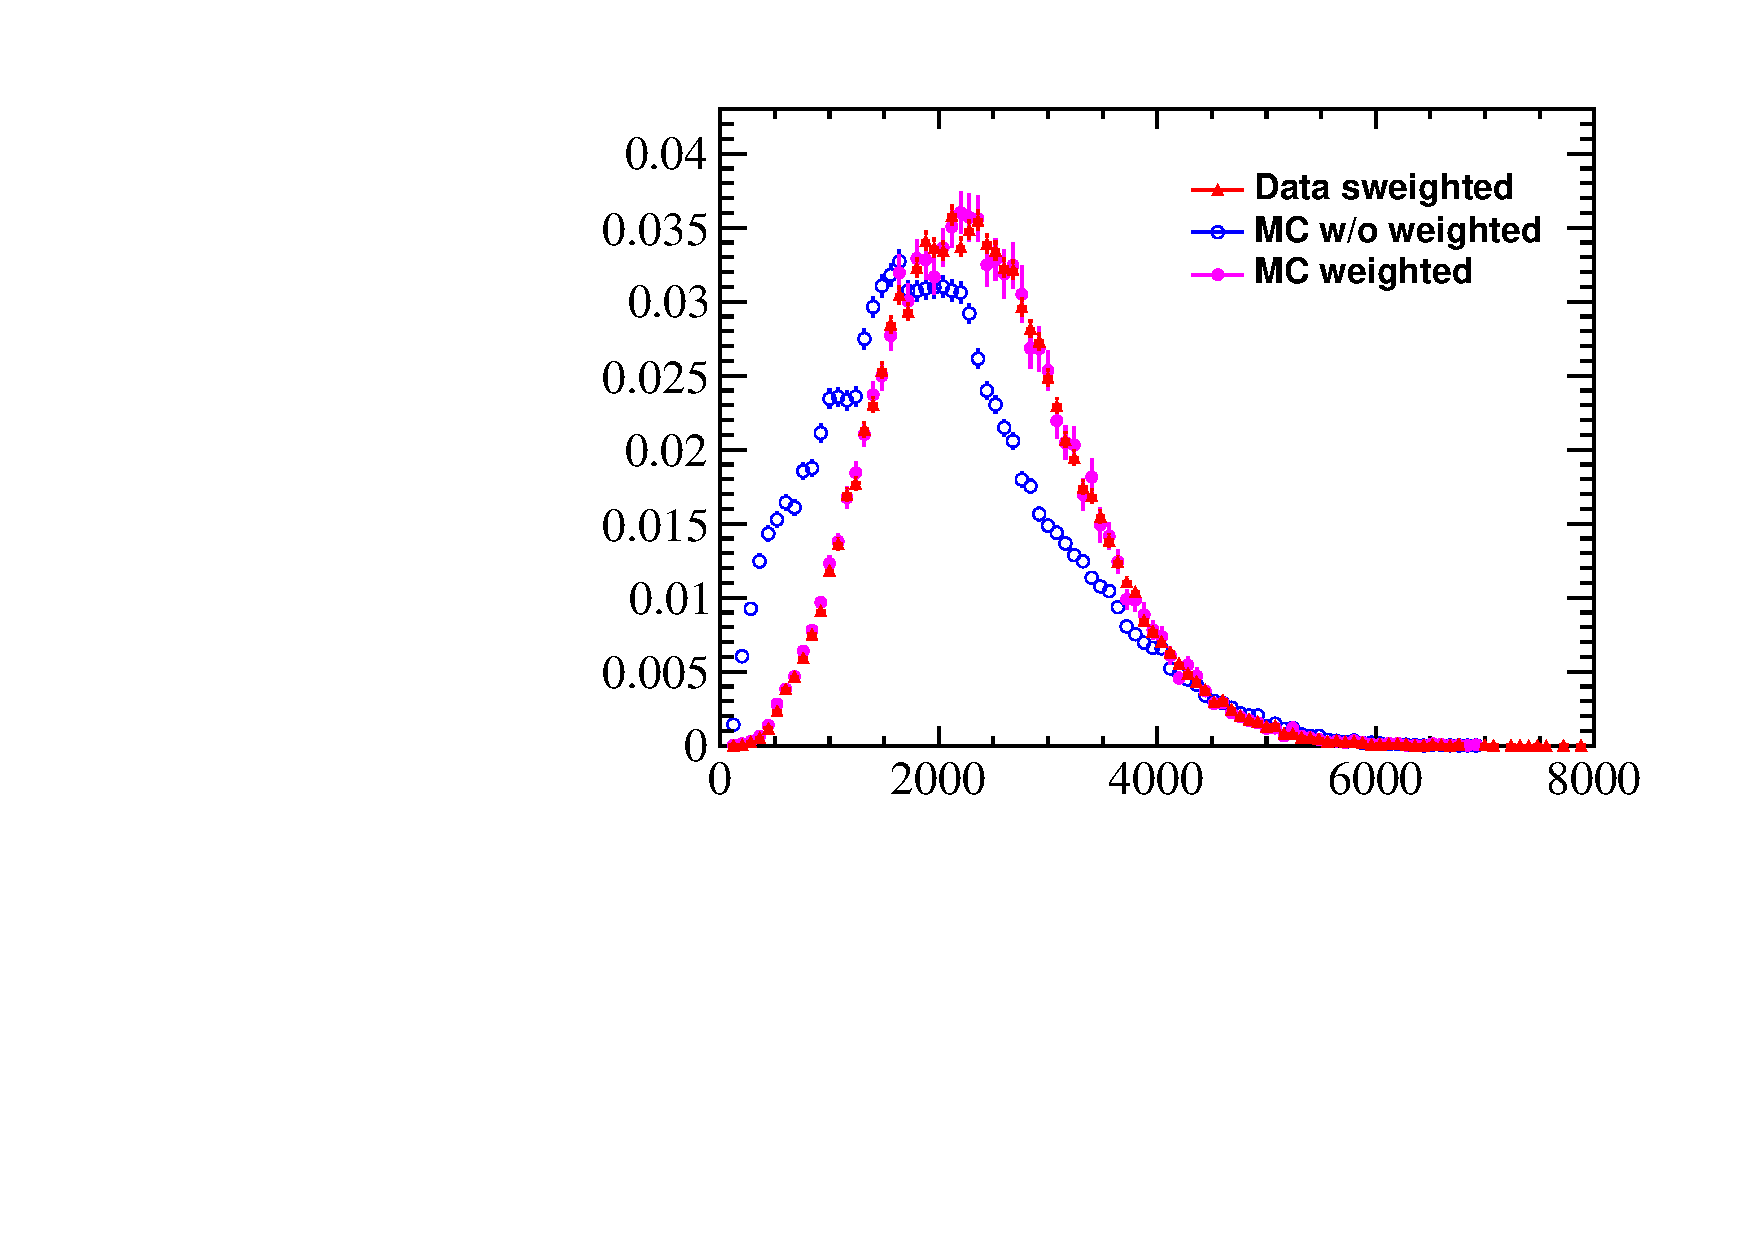
\includegraphics[width=0.45\linewidth]{plots/Lc_comparison/nVeloClusters1}\put(-40,140){(a)}
    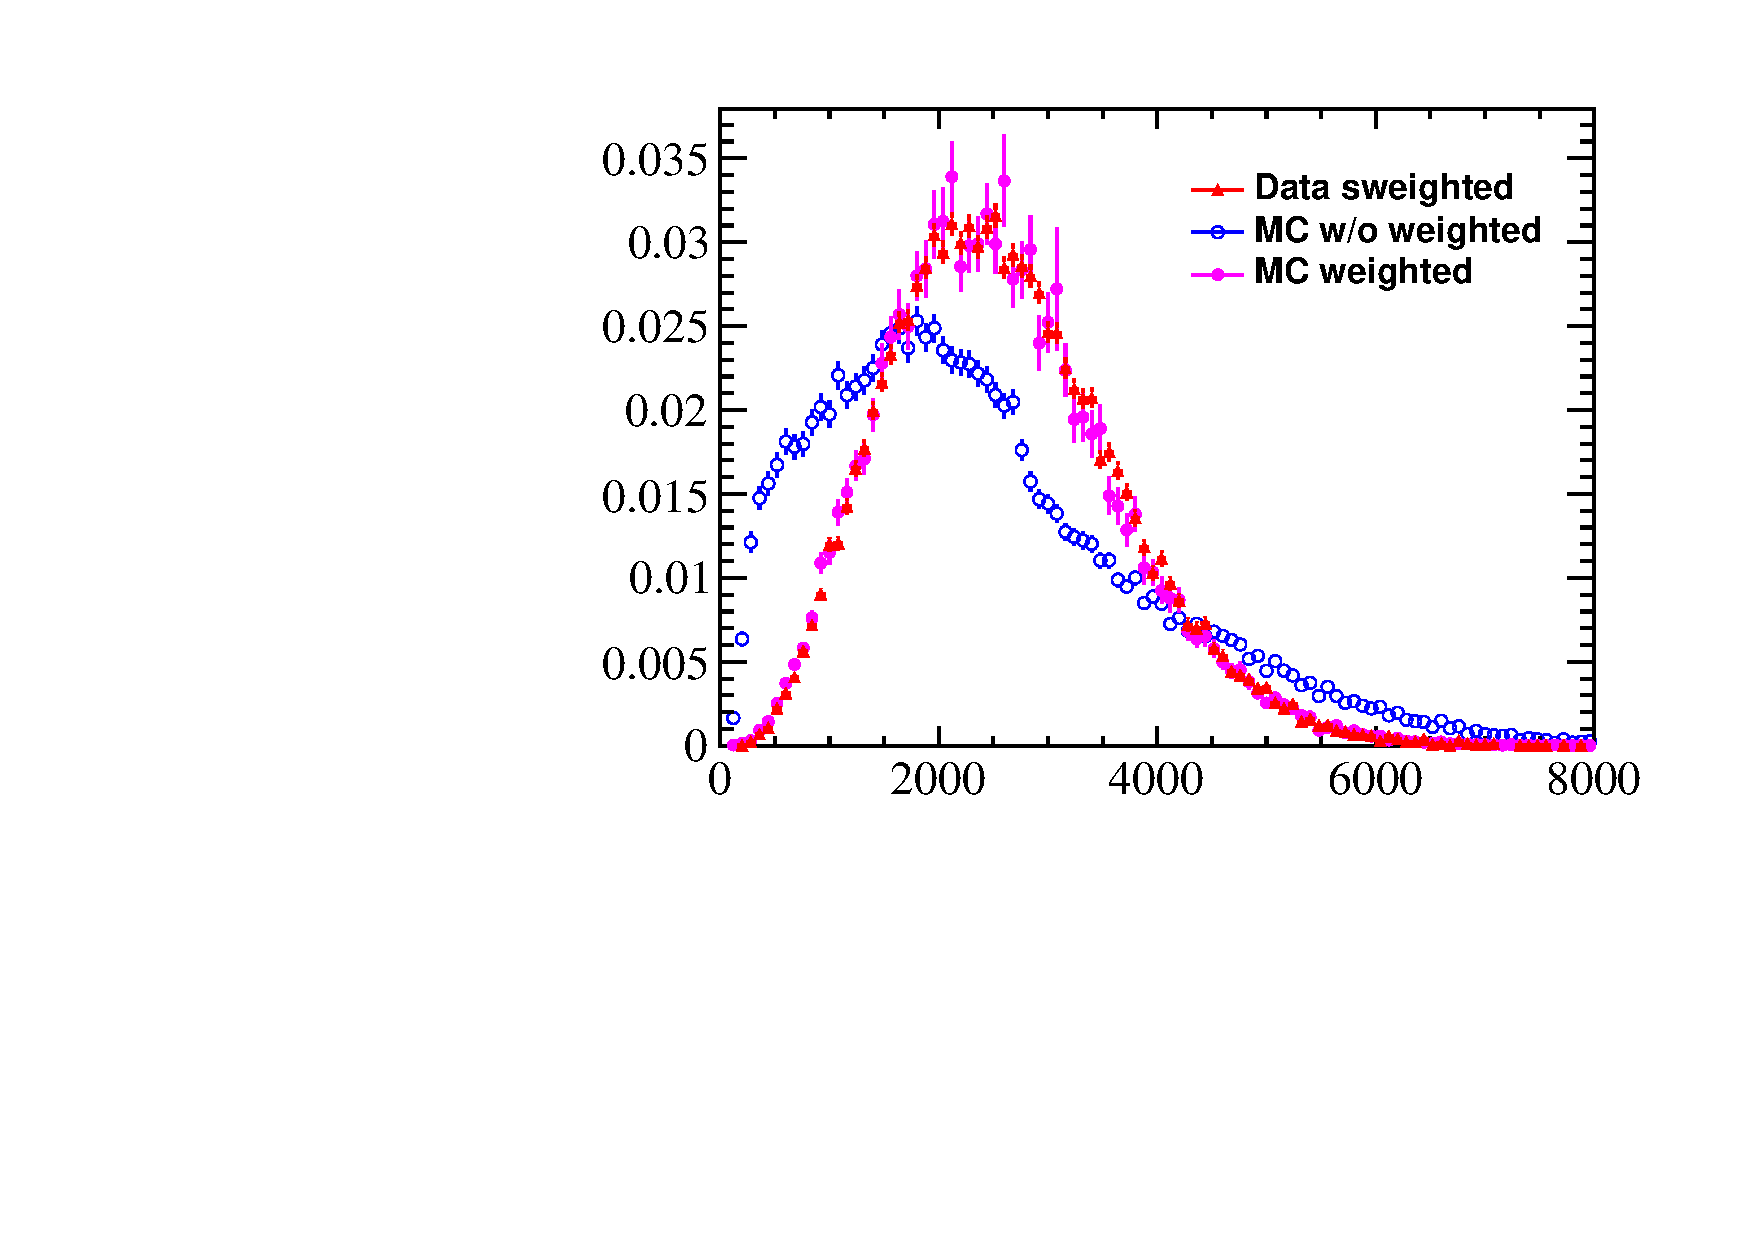
\includegraphics[width=0.45\linewidth]{plots/Lc_comparison/nVeloClusters2}\put(-40,140){(b)}

    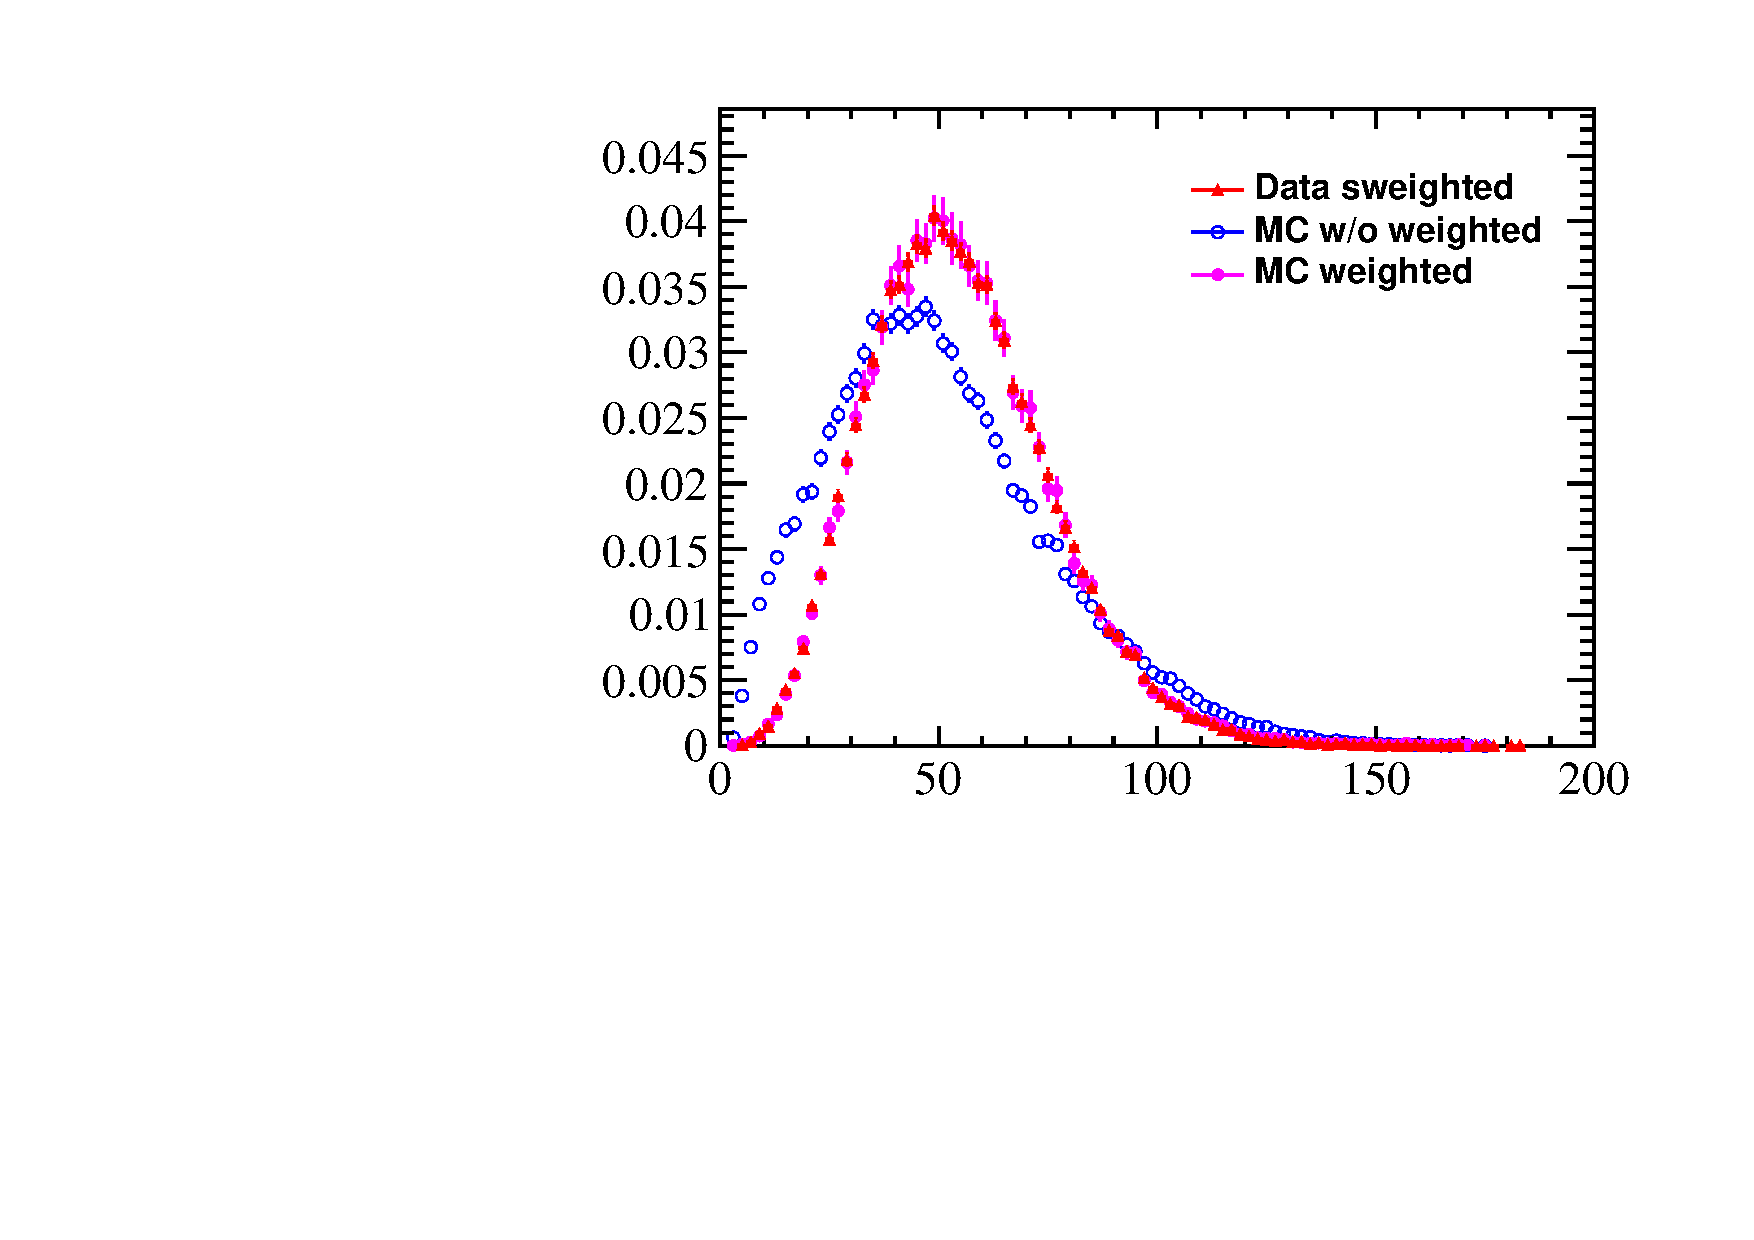
\includegraphics[width=0.45\linewidth]{plots/Lc_comparison/nLongTracks1}\put(-40,140){(c)}
    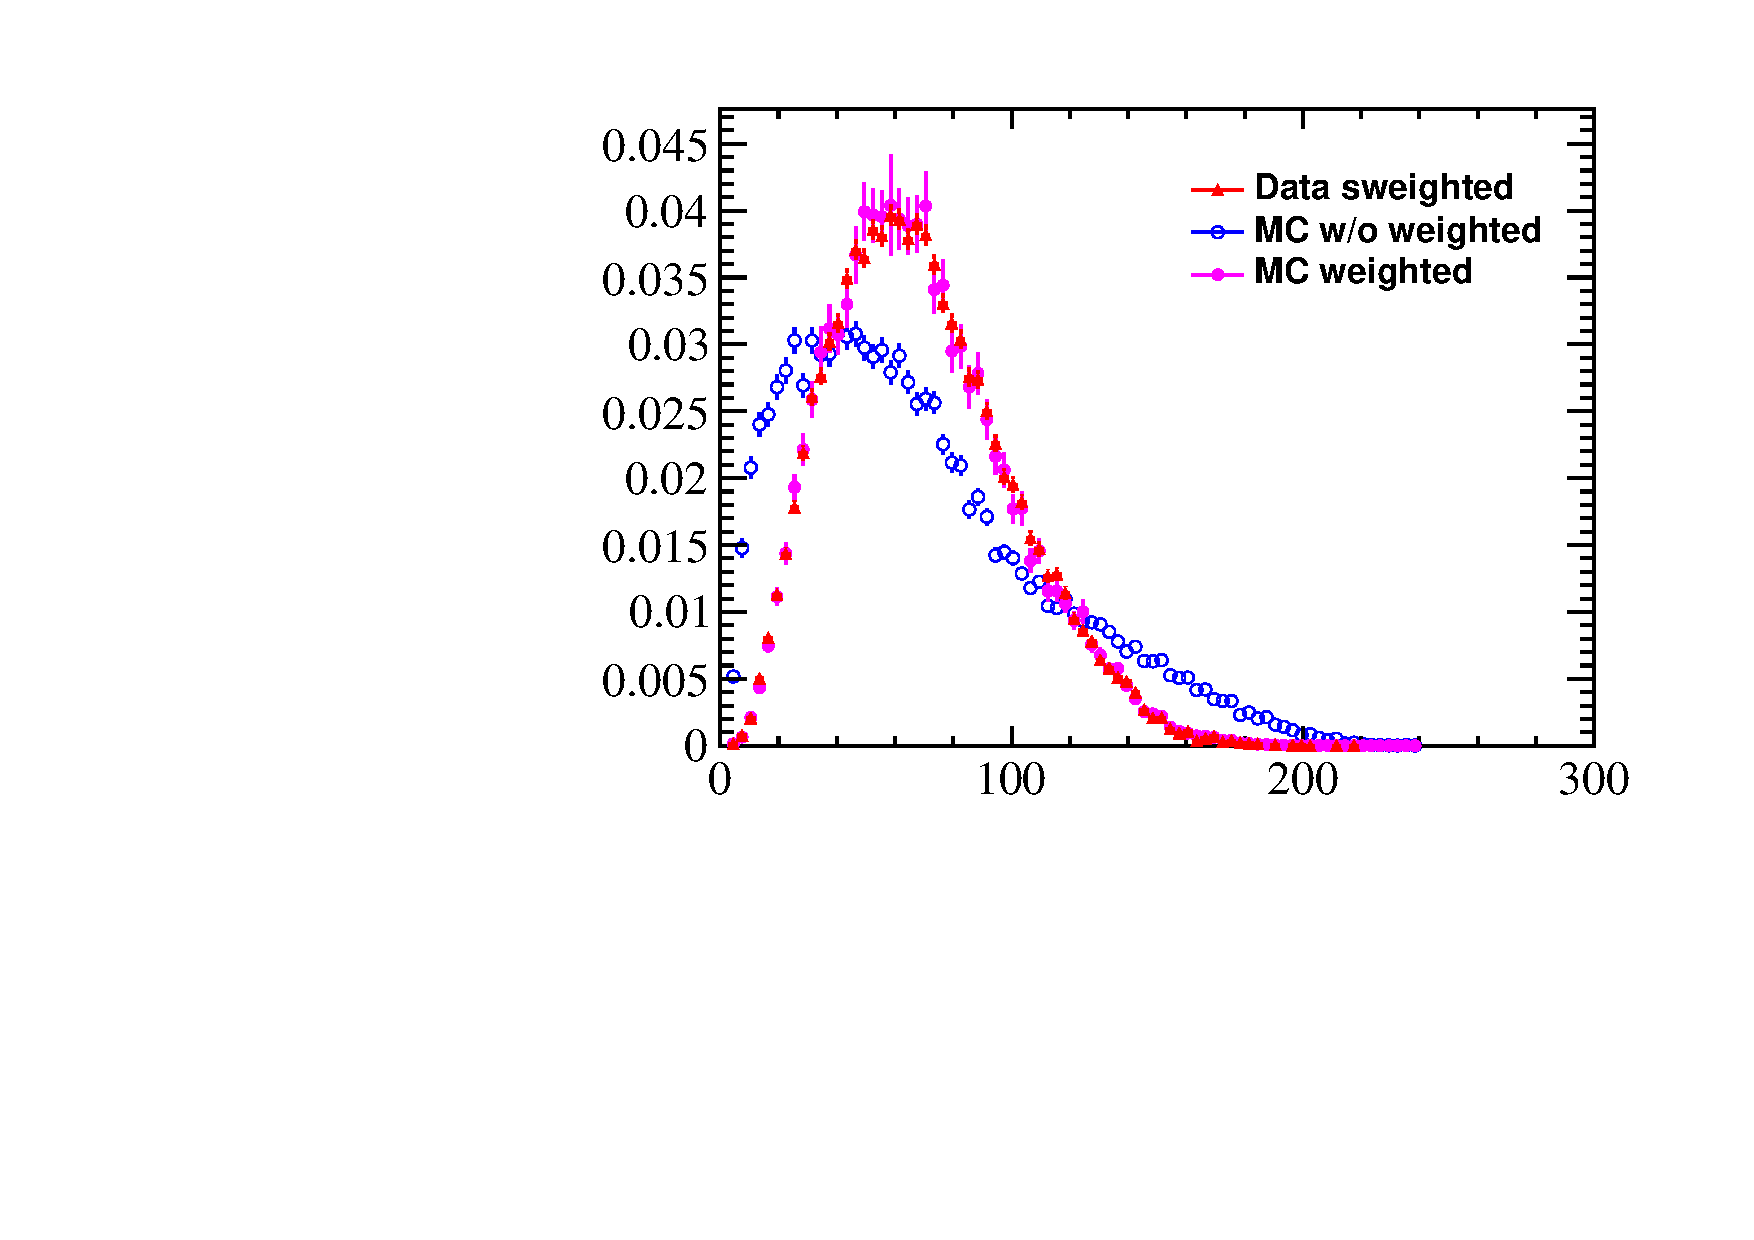
\includegraphics[width=0.45\linewidth]{plots/Lc_comparison/nLongTracks2}\put(-40,140){(d)}

    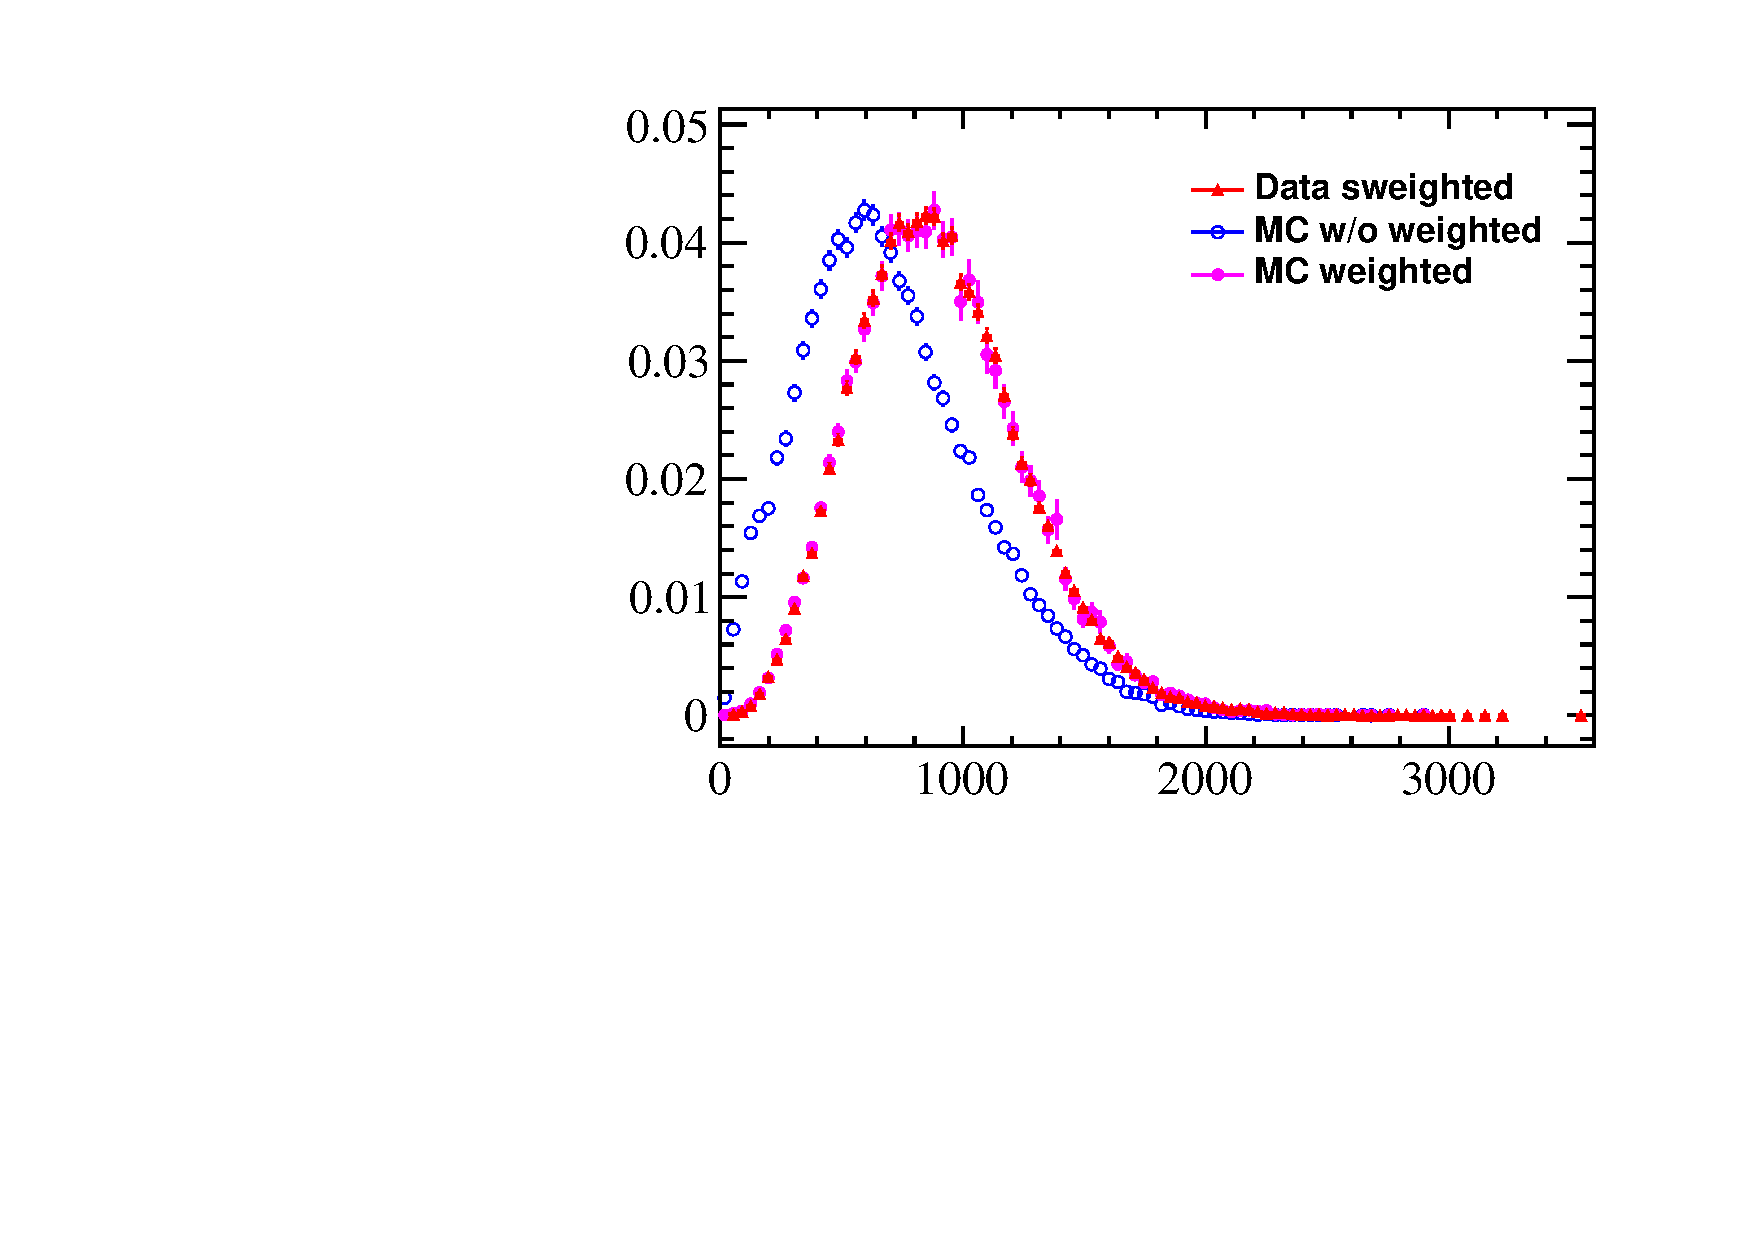
\includegraphics[width=0.45\linewidth]{plots/Lc_comparison/nTTClusters1}\put(-40,140){(e)}
    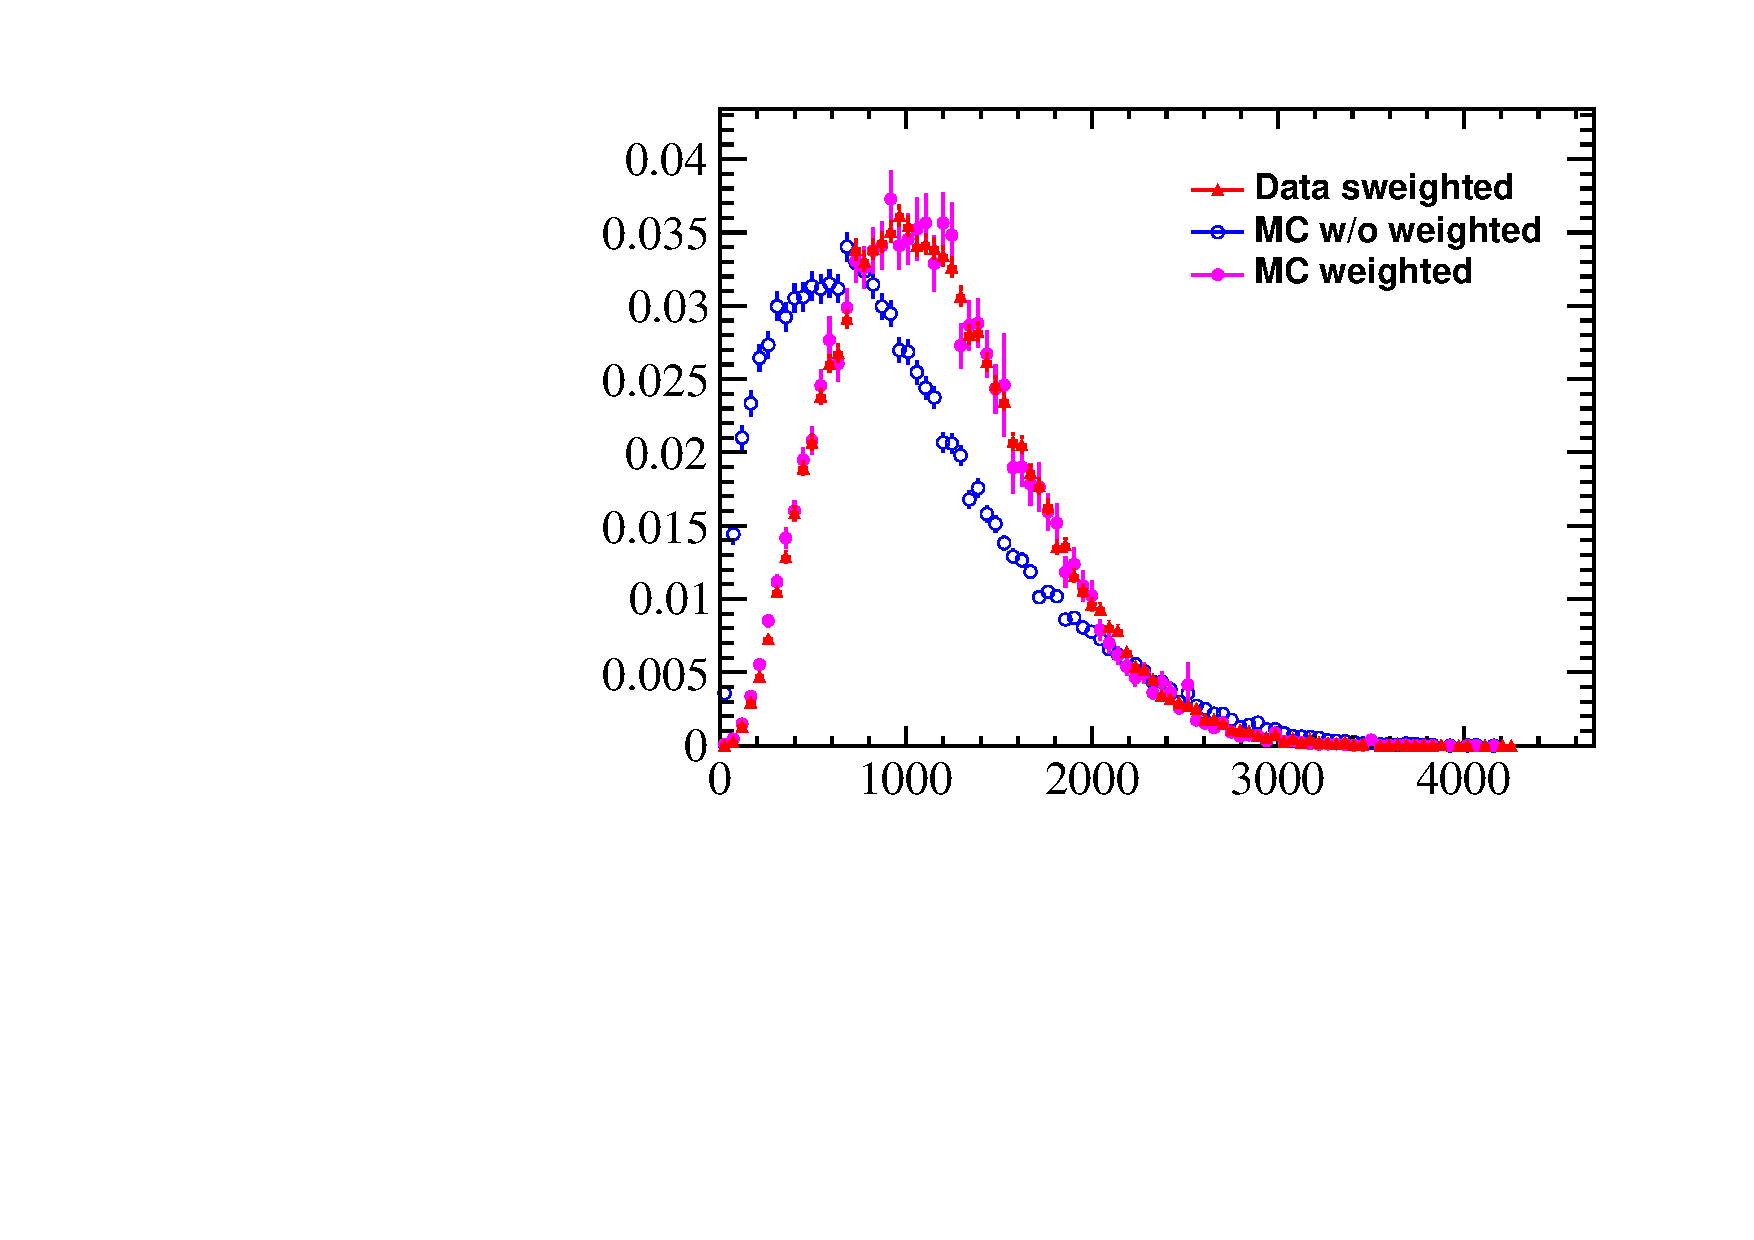
\includegraphics[width=0.45\linewidth]{plots/Lc_comparison/nTTClusters2}\put(-40,140){(f)}
    \vspace*{-0.5cm}
    \caption{\small
    Distributions of multiplicity variables $\nVeloClusters$ (top),
    $\nLongTracks$ (middle) and $\nTTClusters$ (bottom)
    for orignal MC, corrected MC and sWeighted data in (left) forward and (right) backward regions. }
    \label{fig:multiplicity_correction}
\end{figure}

\begin{figure}[htbp]
    \centering
    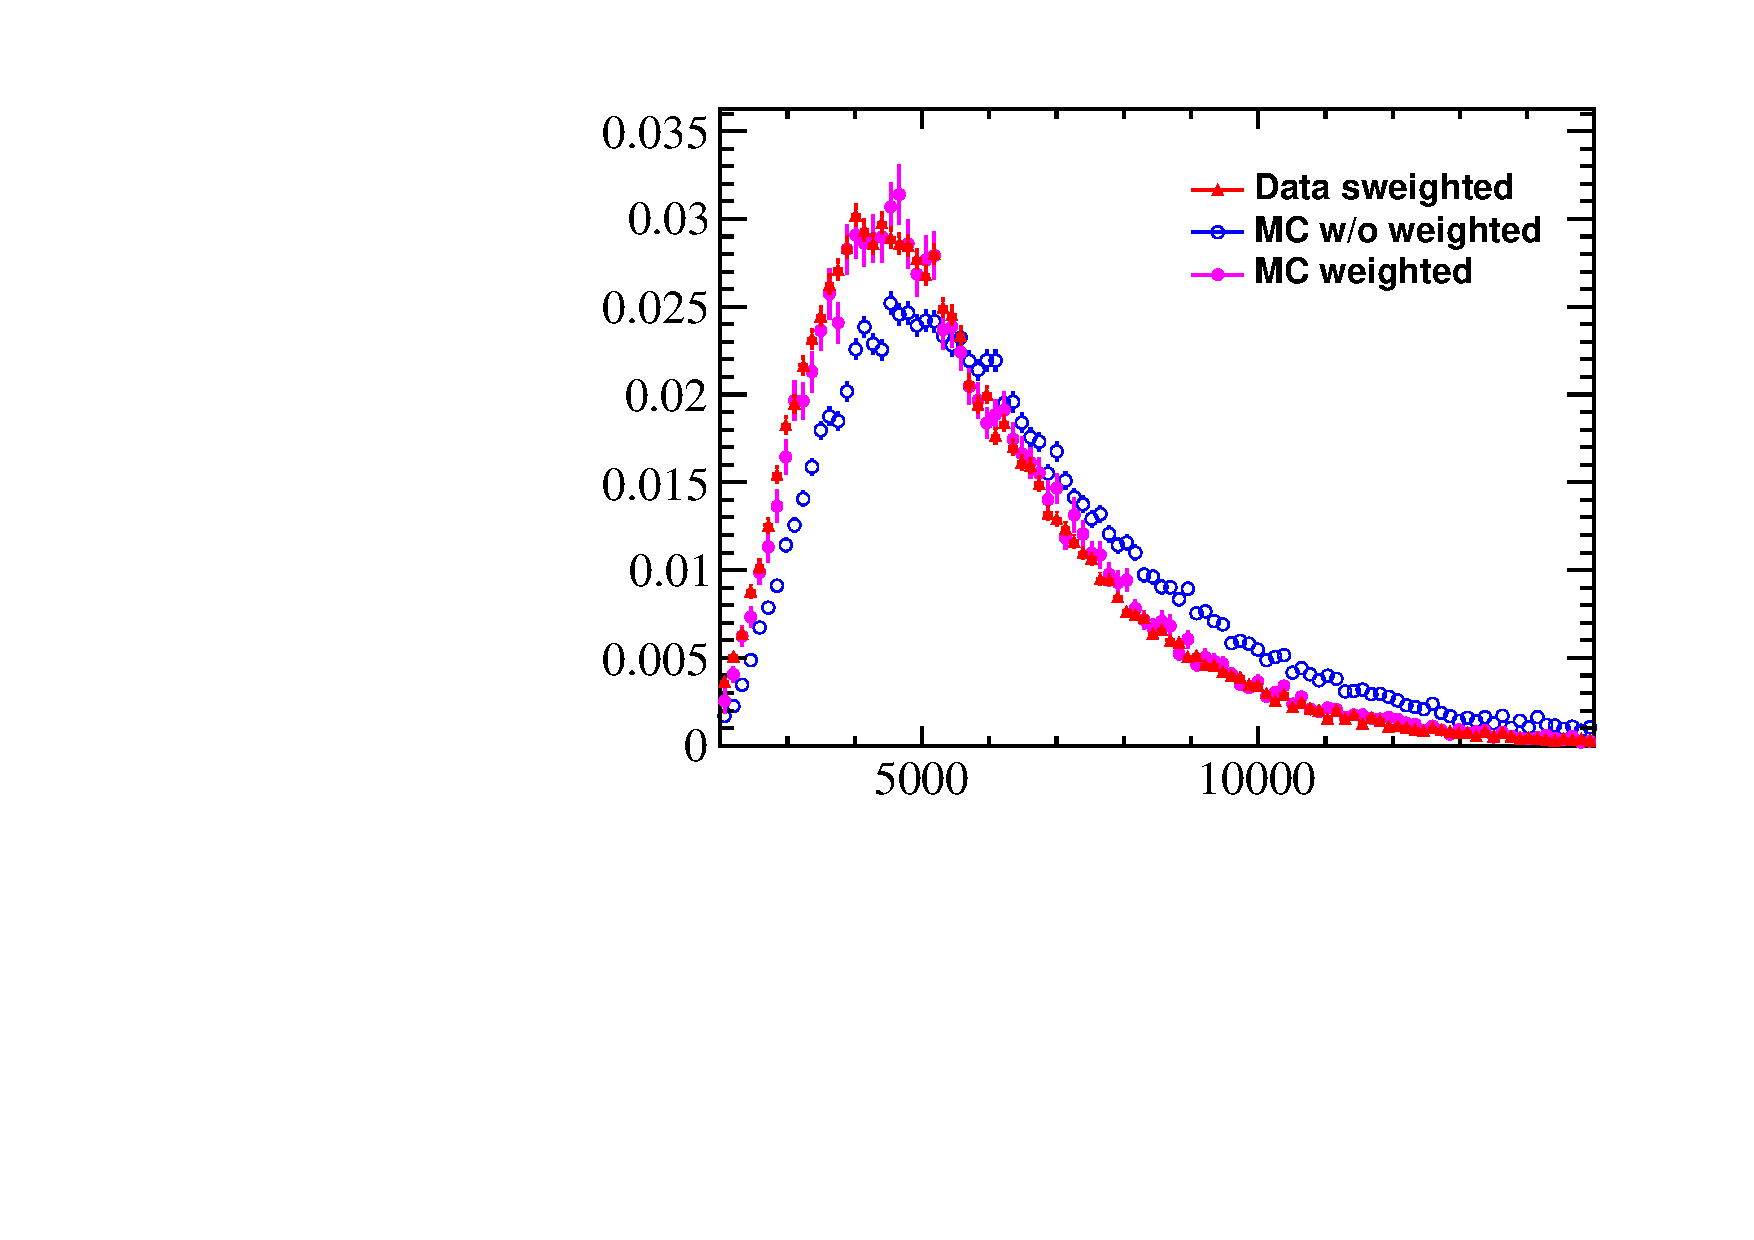
\includegraphics[width=0.45\linewidth]{plots/Lc_comparison/Lc_PT1}\put(-40,140){(a)}
    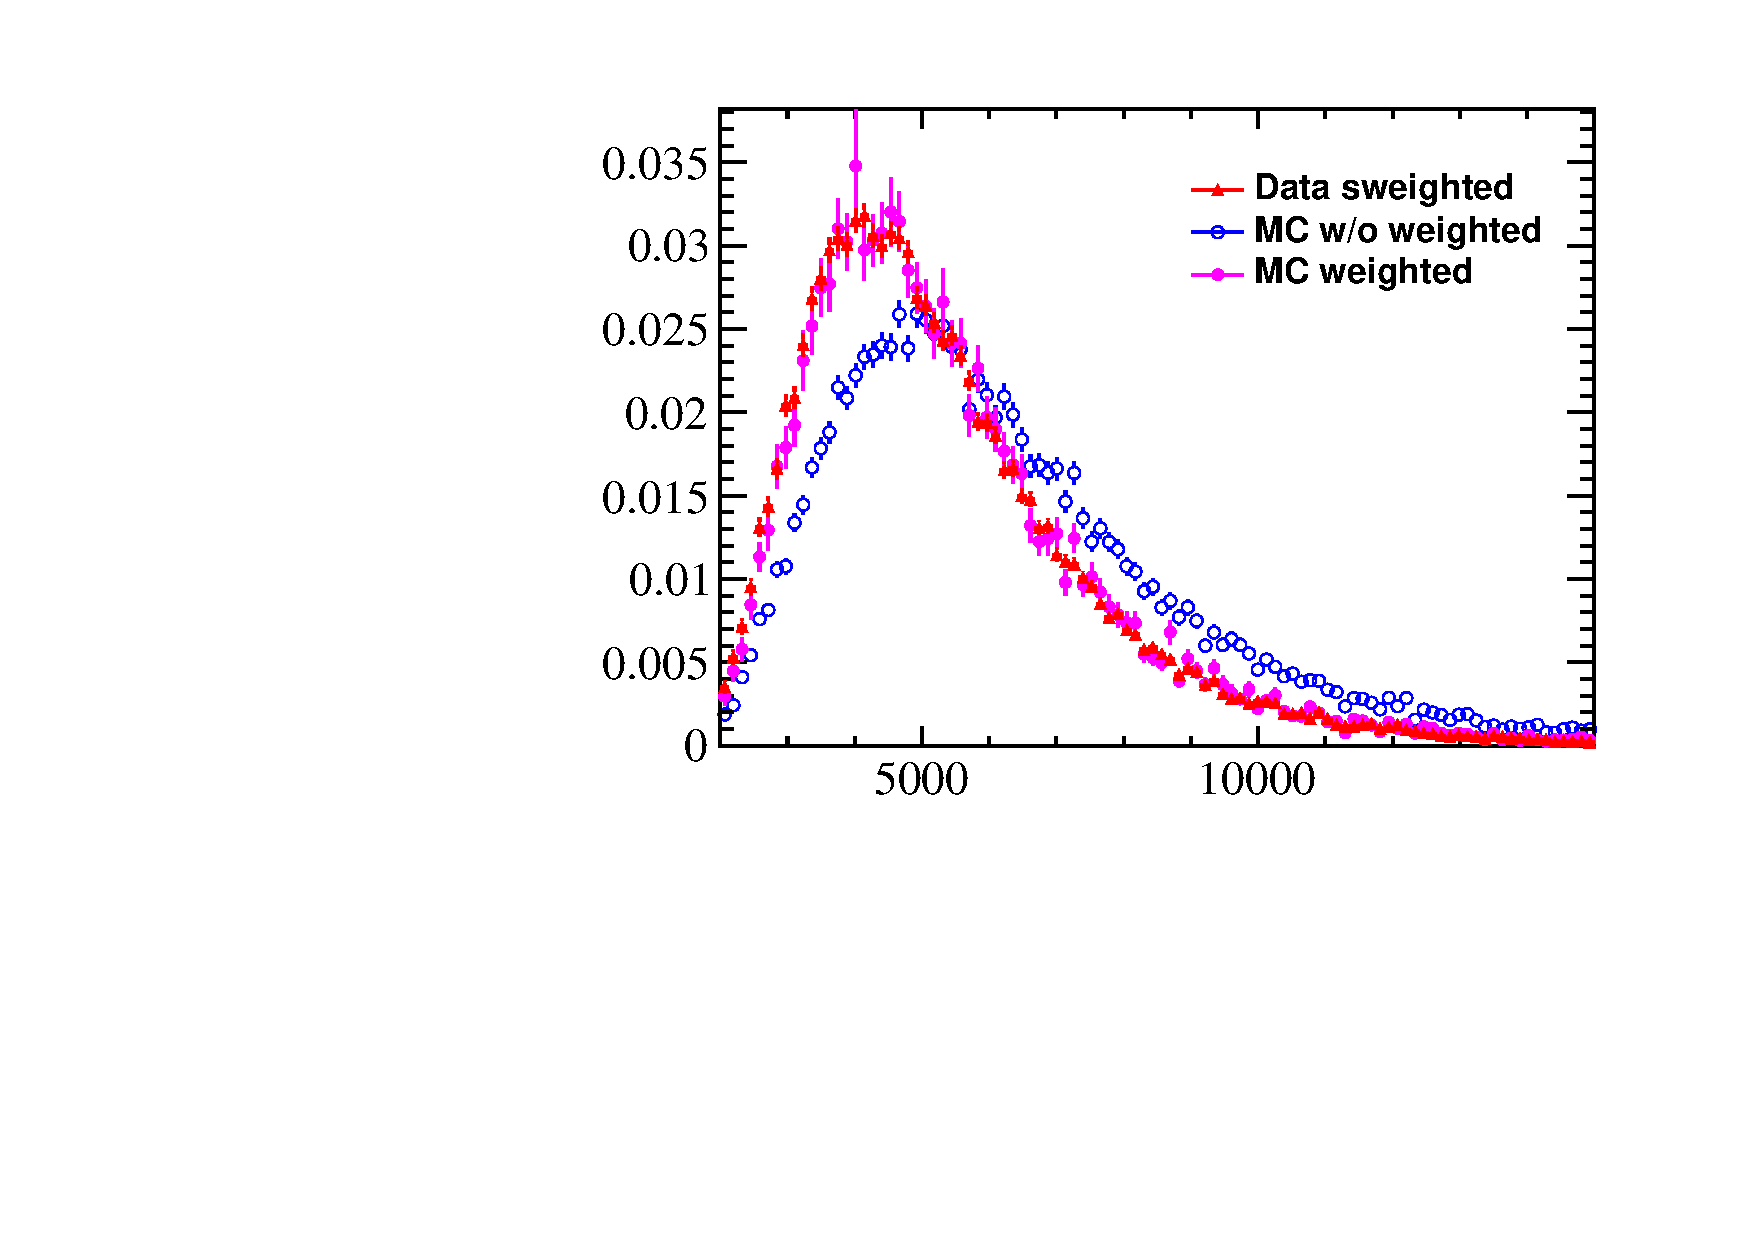
\includegraphics[width=0.45\linewidth]{plots/Lc_comparison/Lc_PT2}\put(-40,140){(b)}

    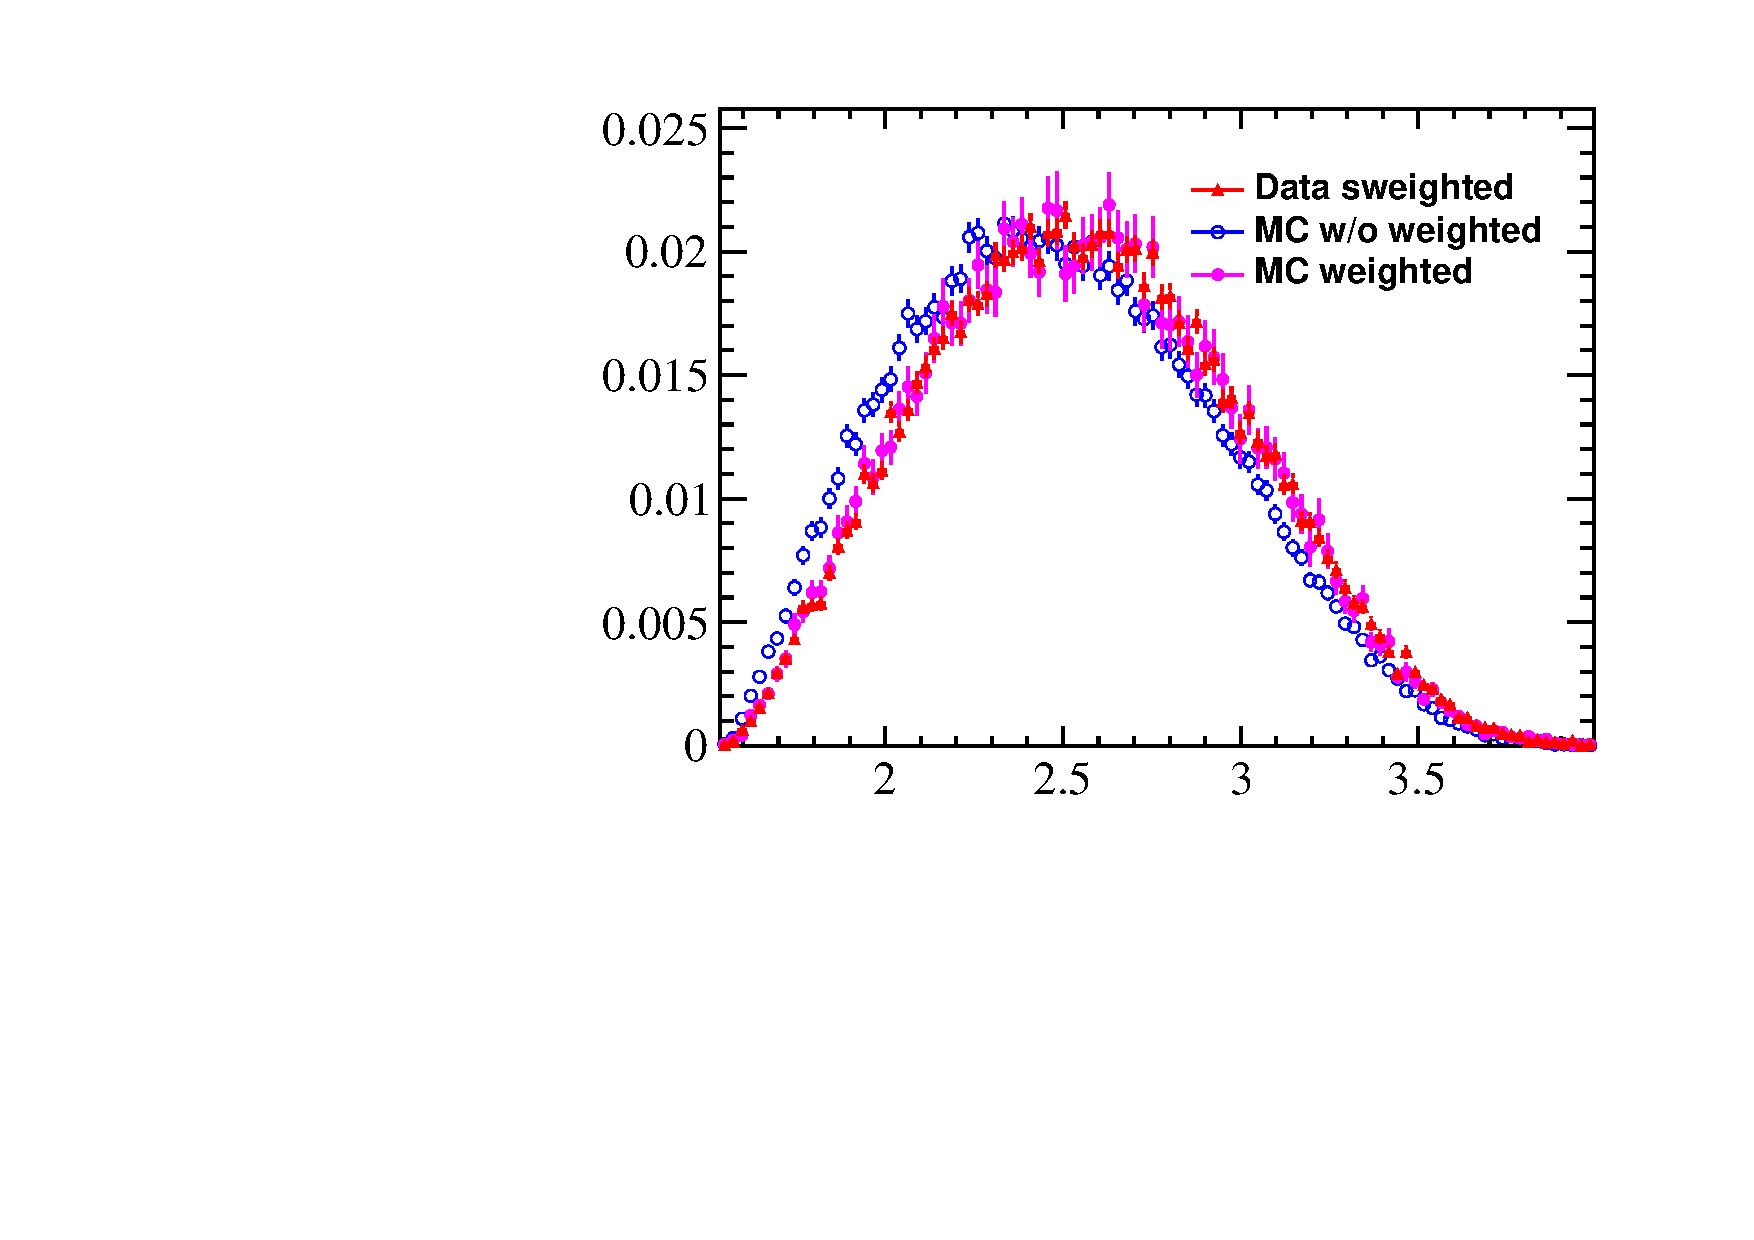
\includegraphics[width=0.45\linewidth]{plots/Lc_comparison/Lc_Ystar1}\put(-40,140){(c)}
    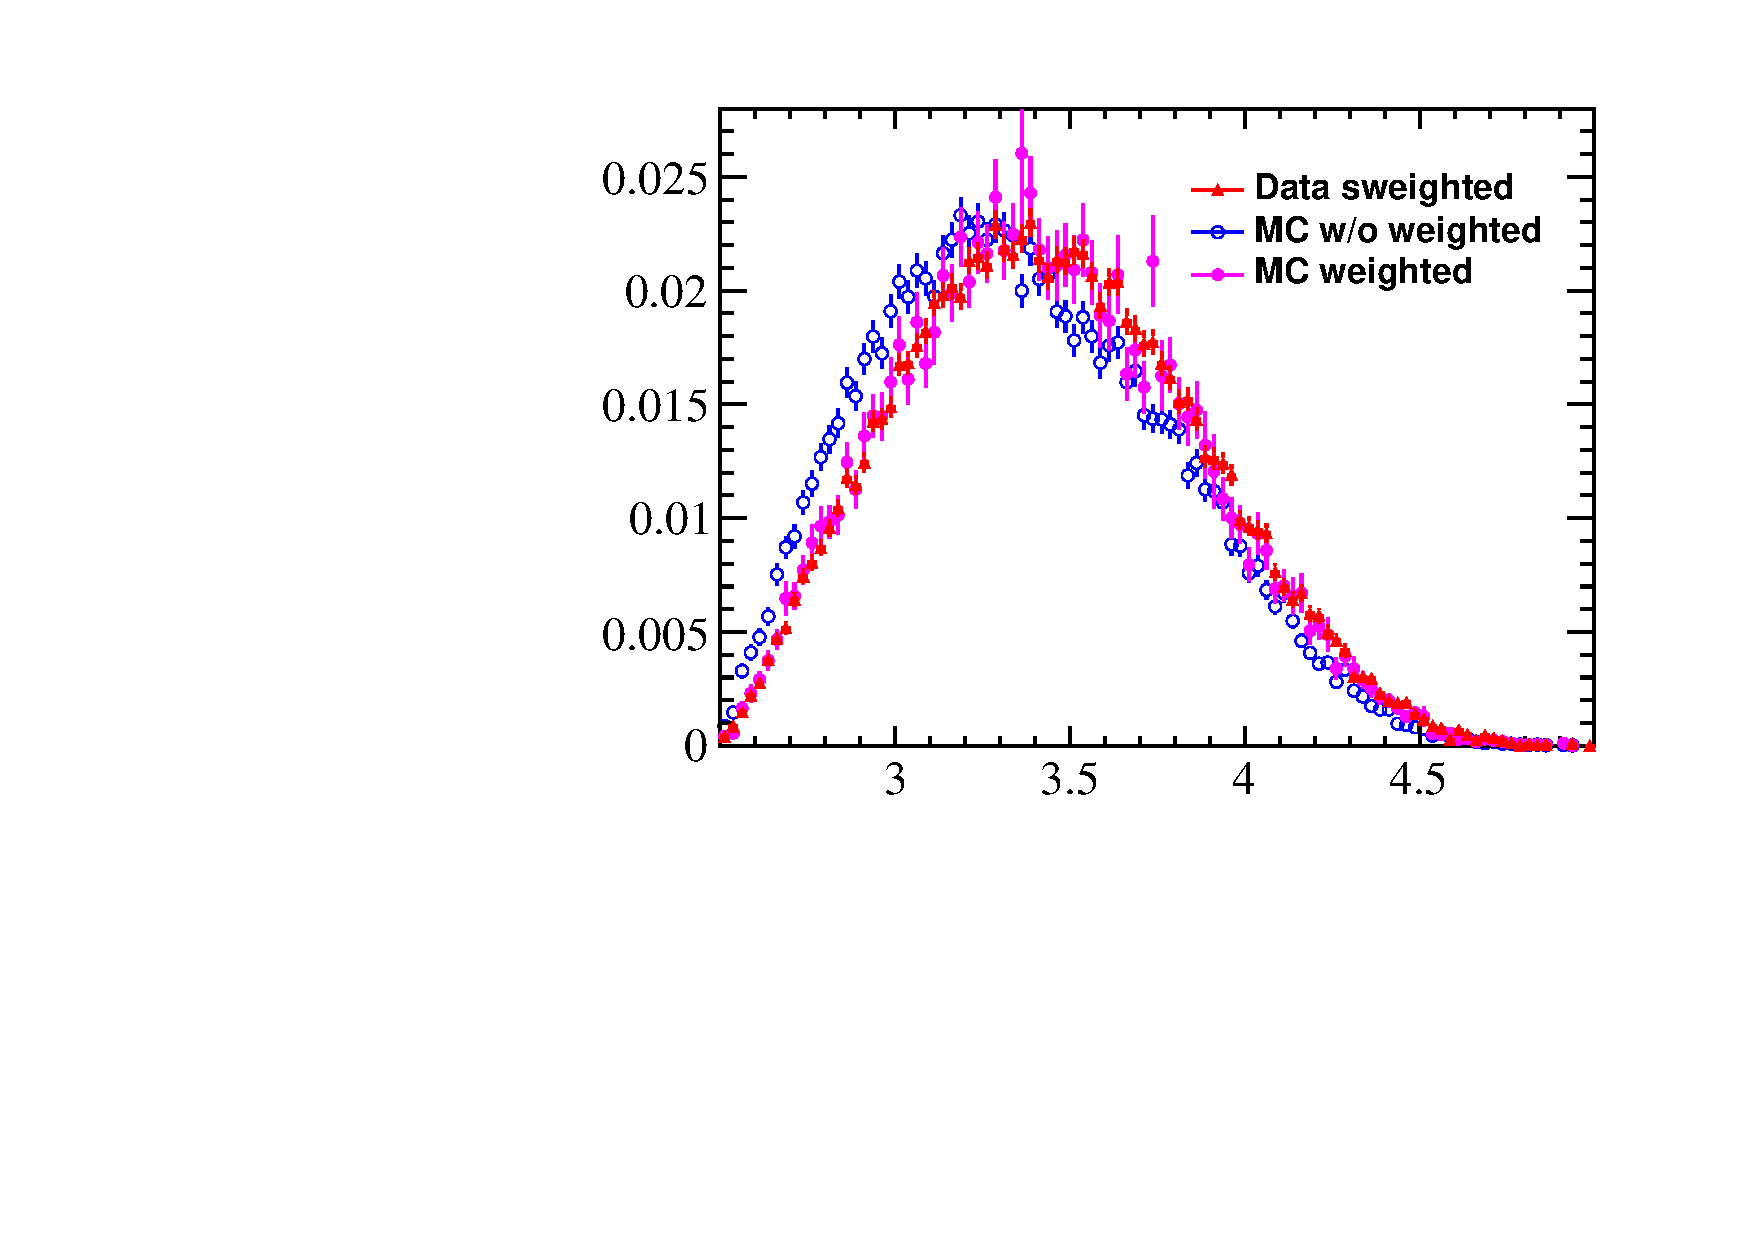
\includegraphics[width=0.45\linewidth]{plots/Lc_comparison/Lc_Ystar2}\put(-40,140){(d)}
    \vspace*{-0.5cm}
    \caption{\small
    Distributions of multiplicity variables $\pt(\Lc)$ (top) and $y^*(\Lc)$ (bottom)
    for orignal MC, corrected MC and sWeighted data in (left) forward and (right) backward regions. }
    \label{fig:kinematic_correction}
\end{figure}

\begin{figure}[htbp]
    \centering
    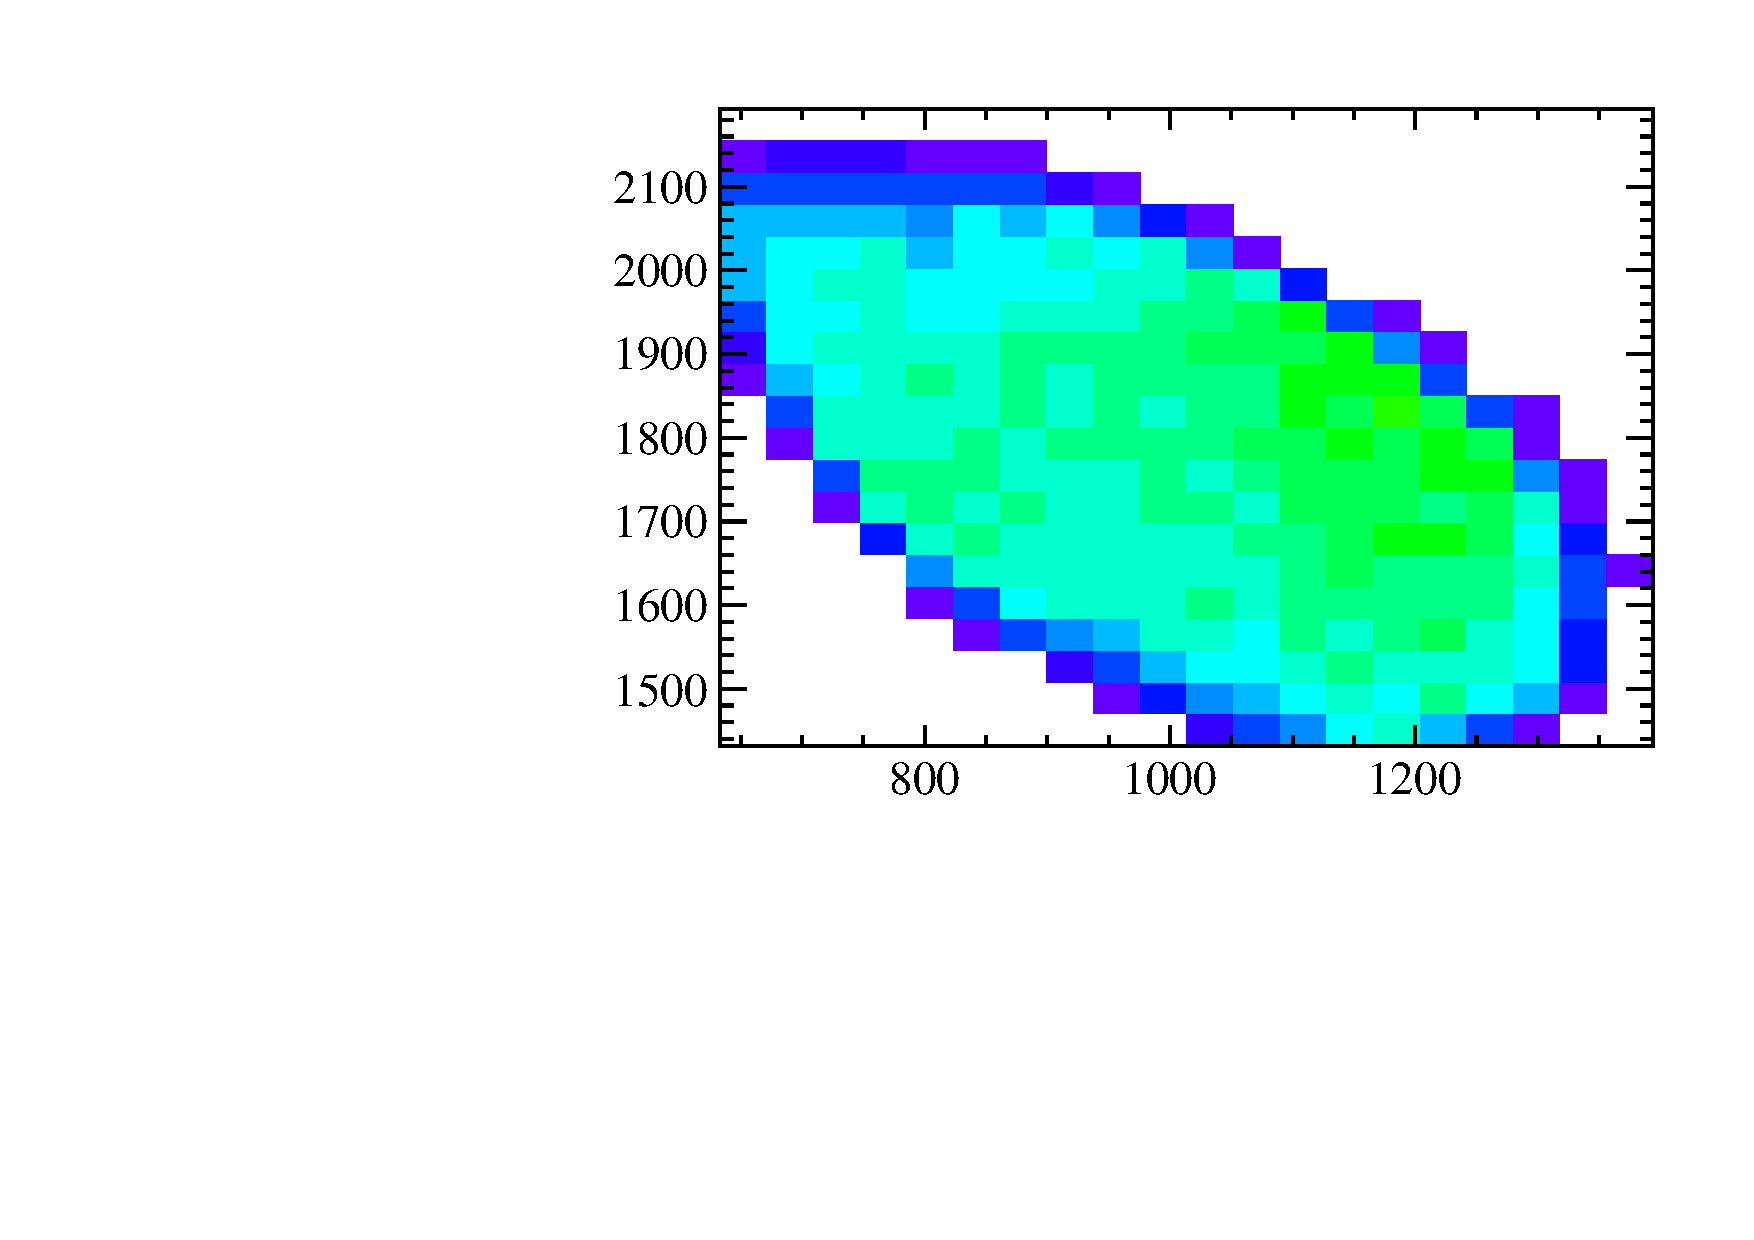
\includegraphics[width=0.45\linewidth]{plots/Lc_comparison/Lc_dalitz_original1}\put(-40,140){(a)}
    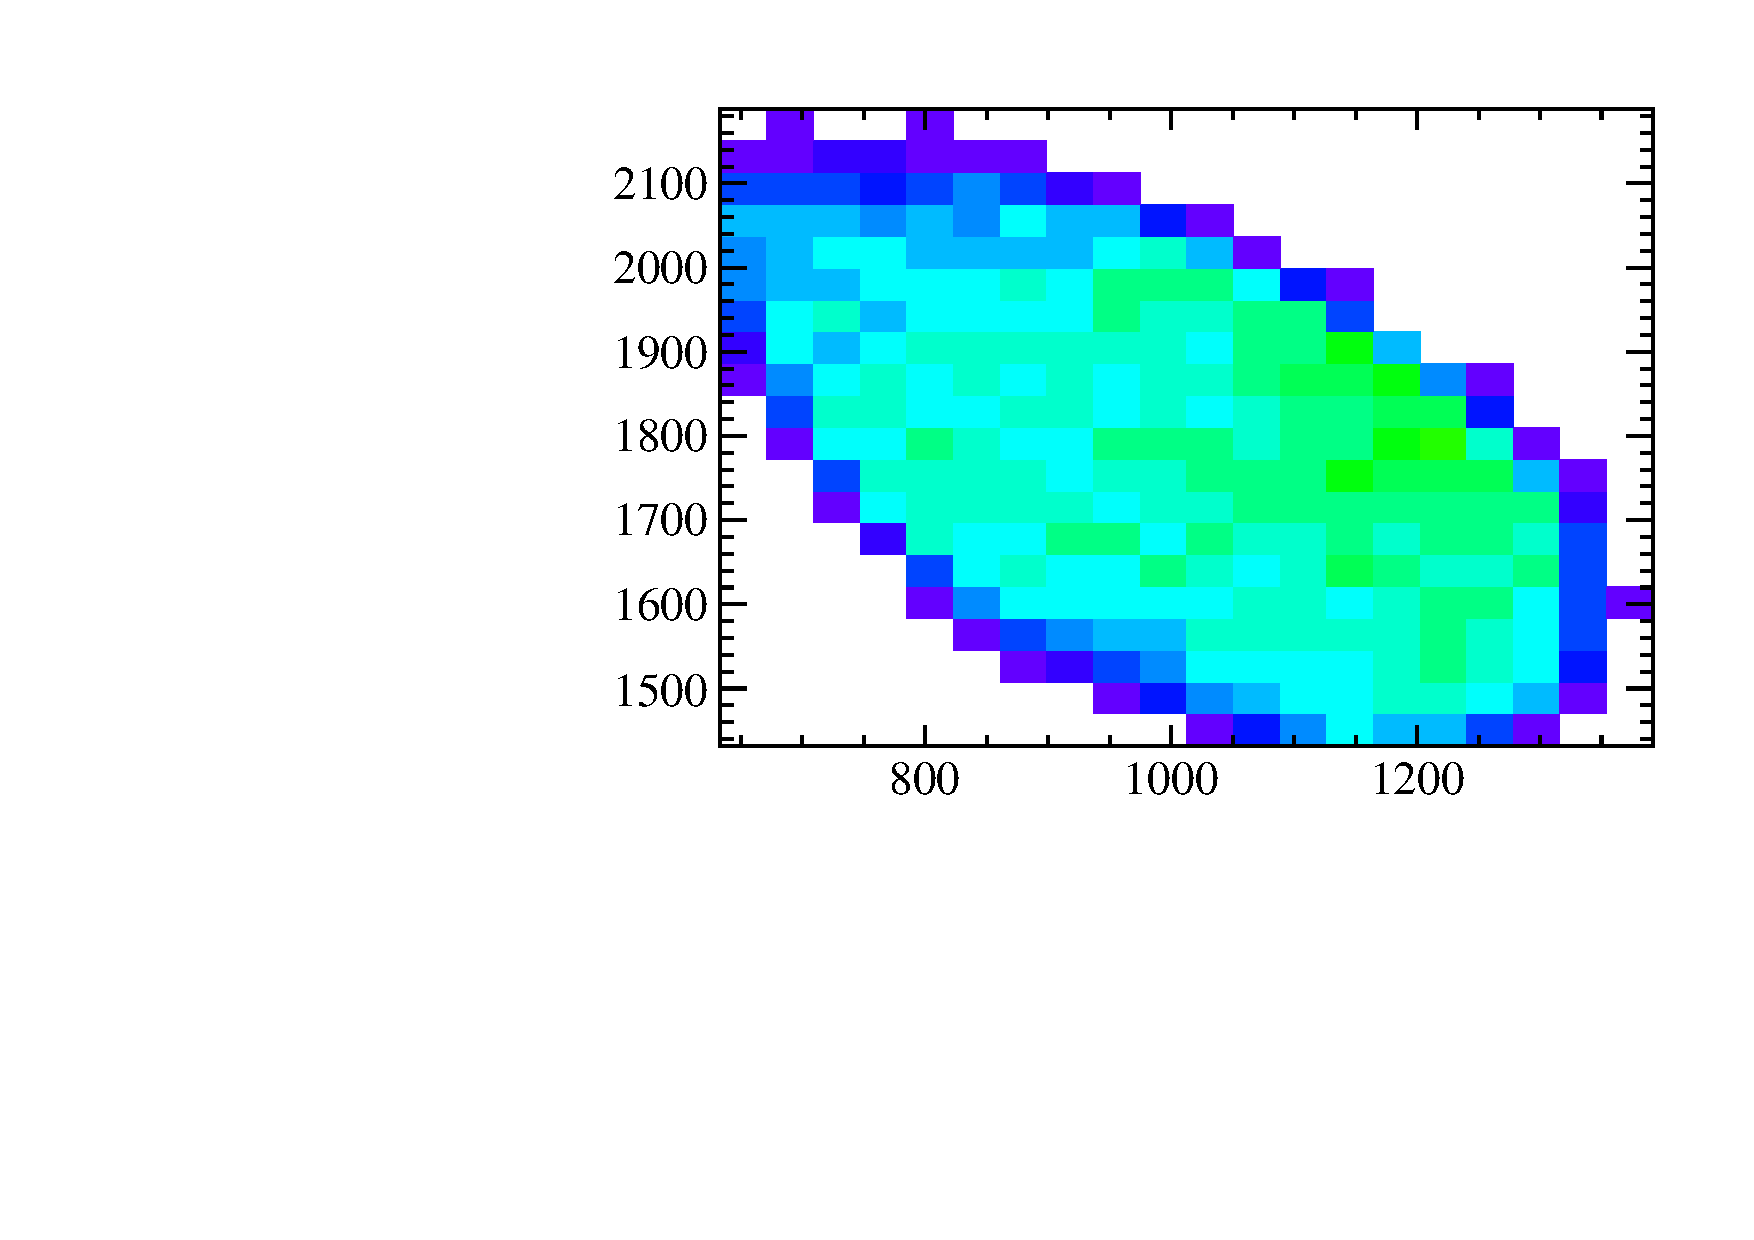
\includegraphics[width=0.45\linewidth]{plots/Lc_comparison/Lc_dalitz_original2}\put(-40,140){(b)}

    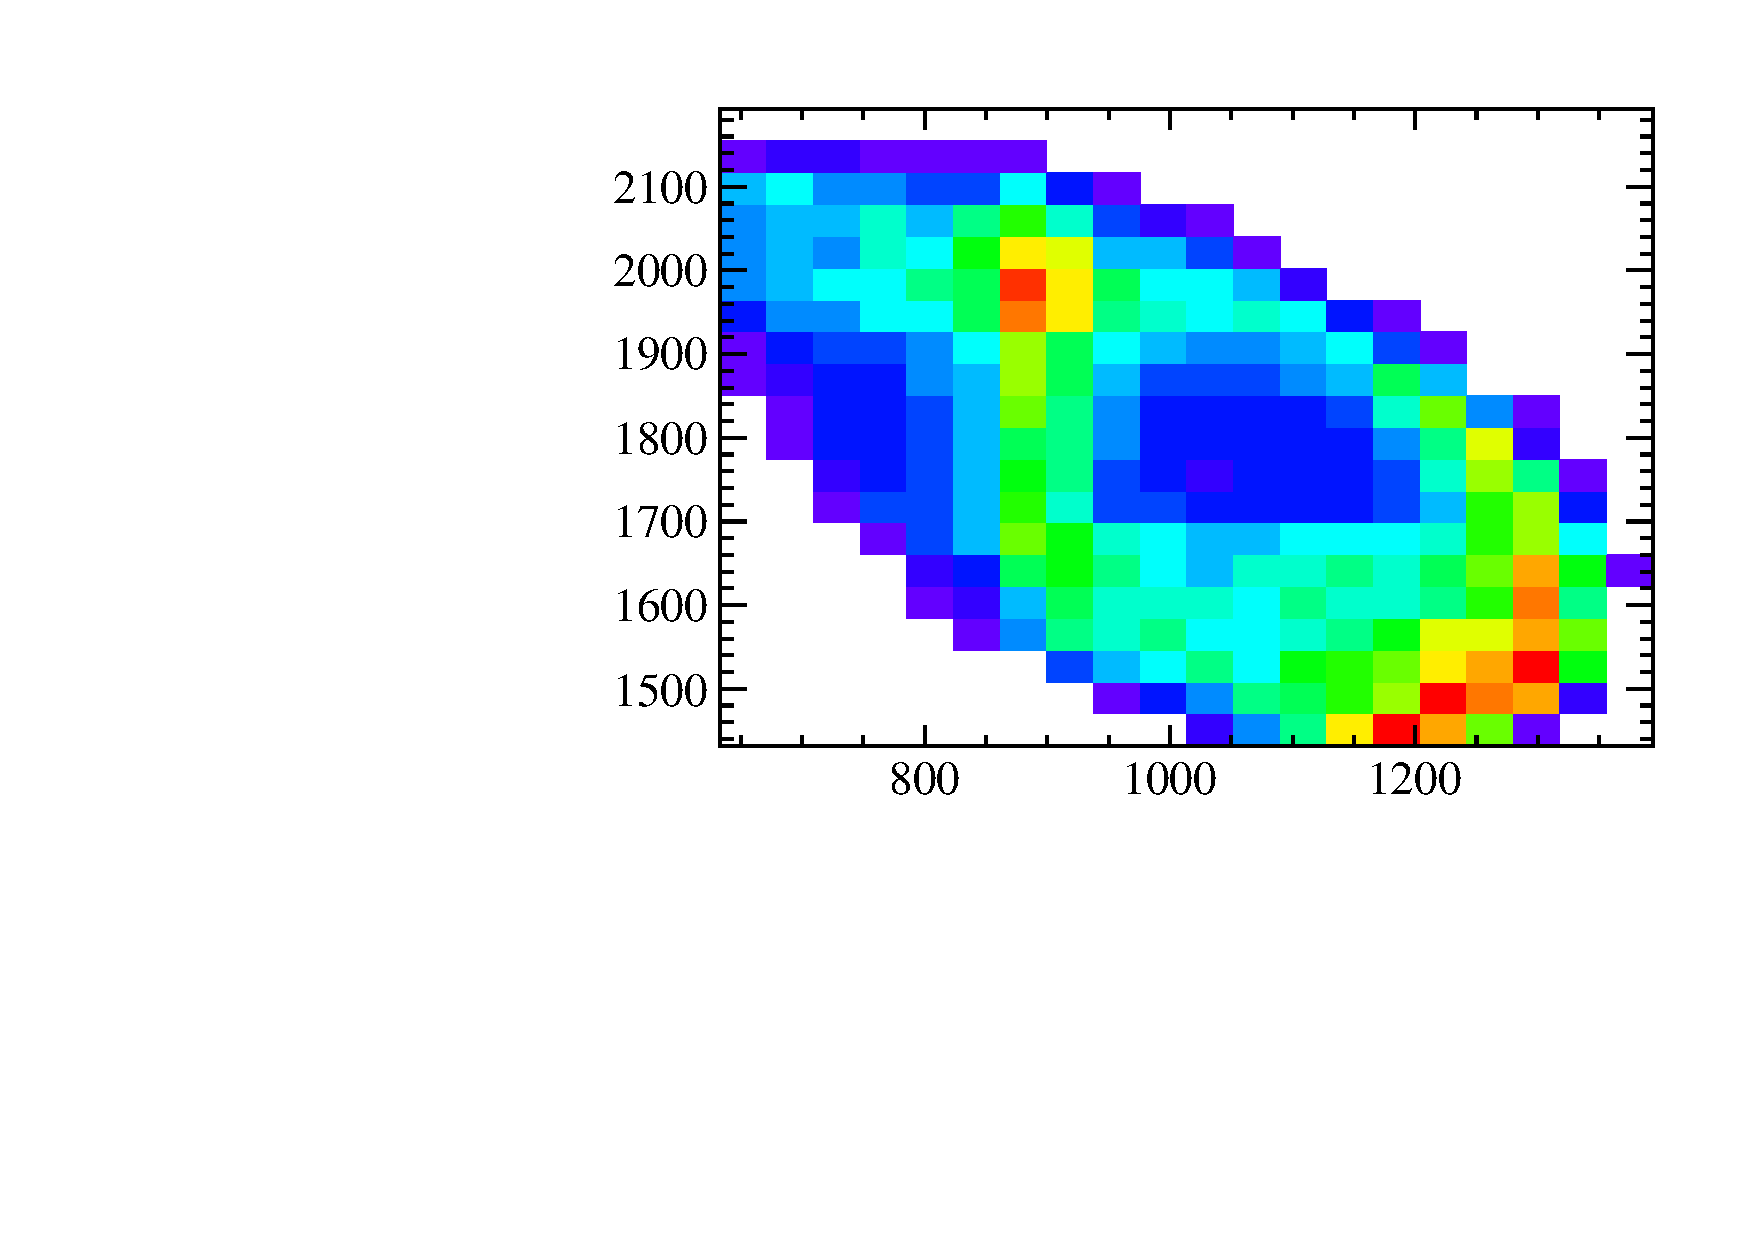
\includegraphics[width=0.45\linewidth]{plots/Lc_comparison/Lc_dalitz_reweight1}\put(-40,140){(c)}
    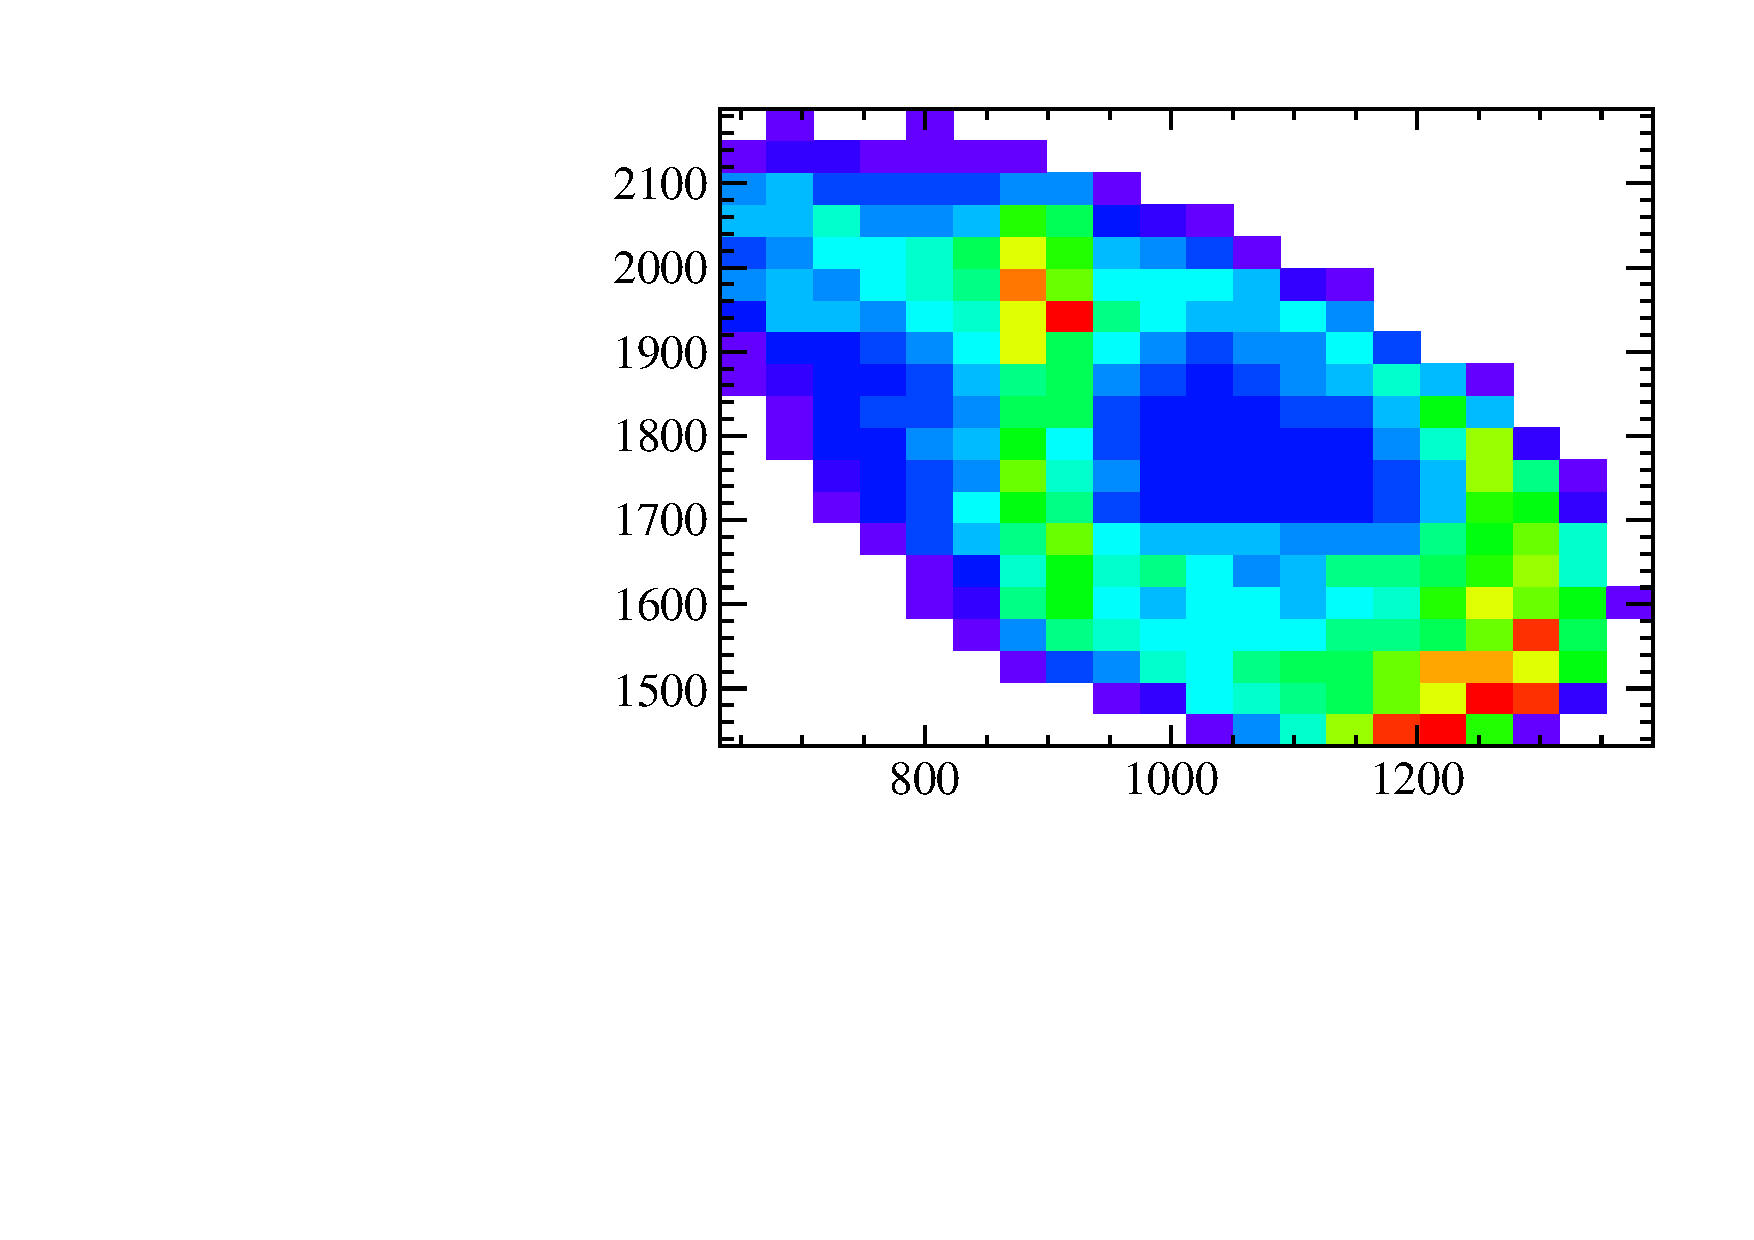
\includegraphics[width=0.45\linewidth]{plots/Lc_comparison/Lc_dalitz_reweight2}\put(-40,140){(d)}

    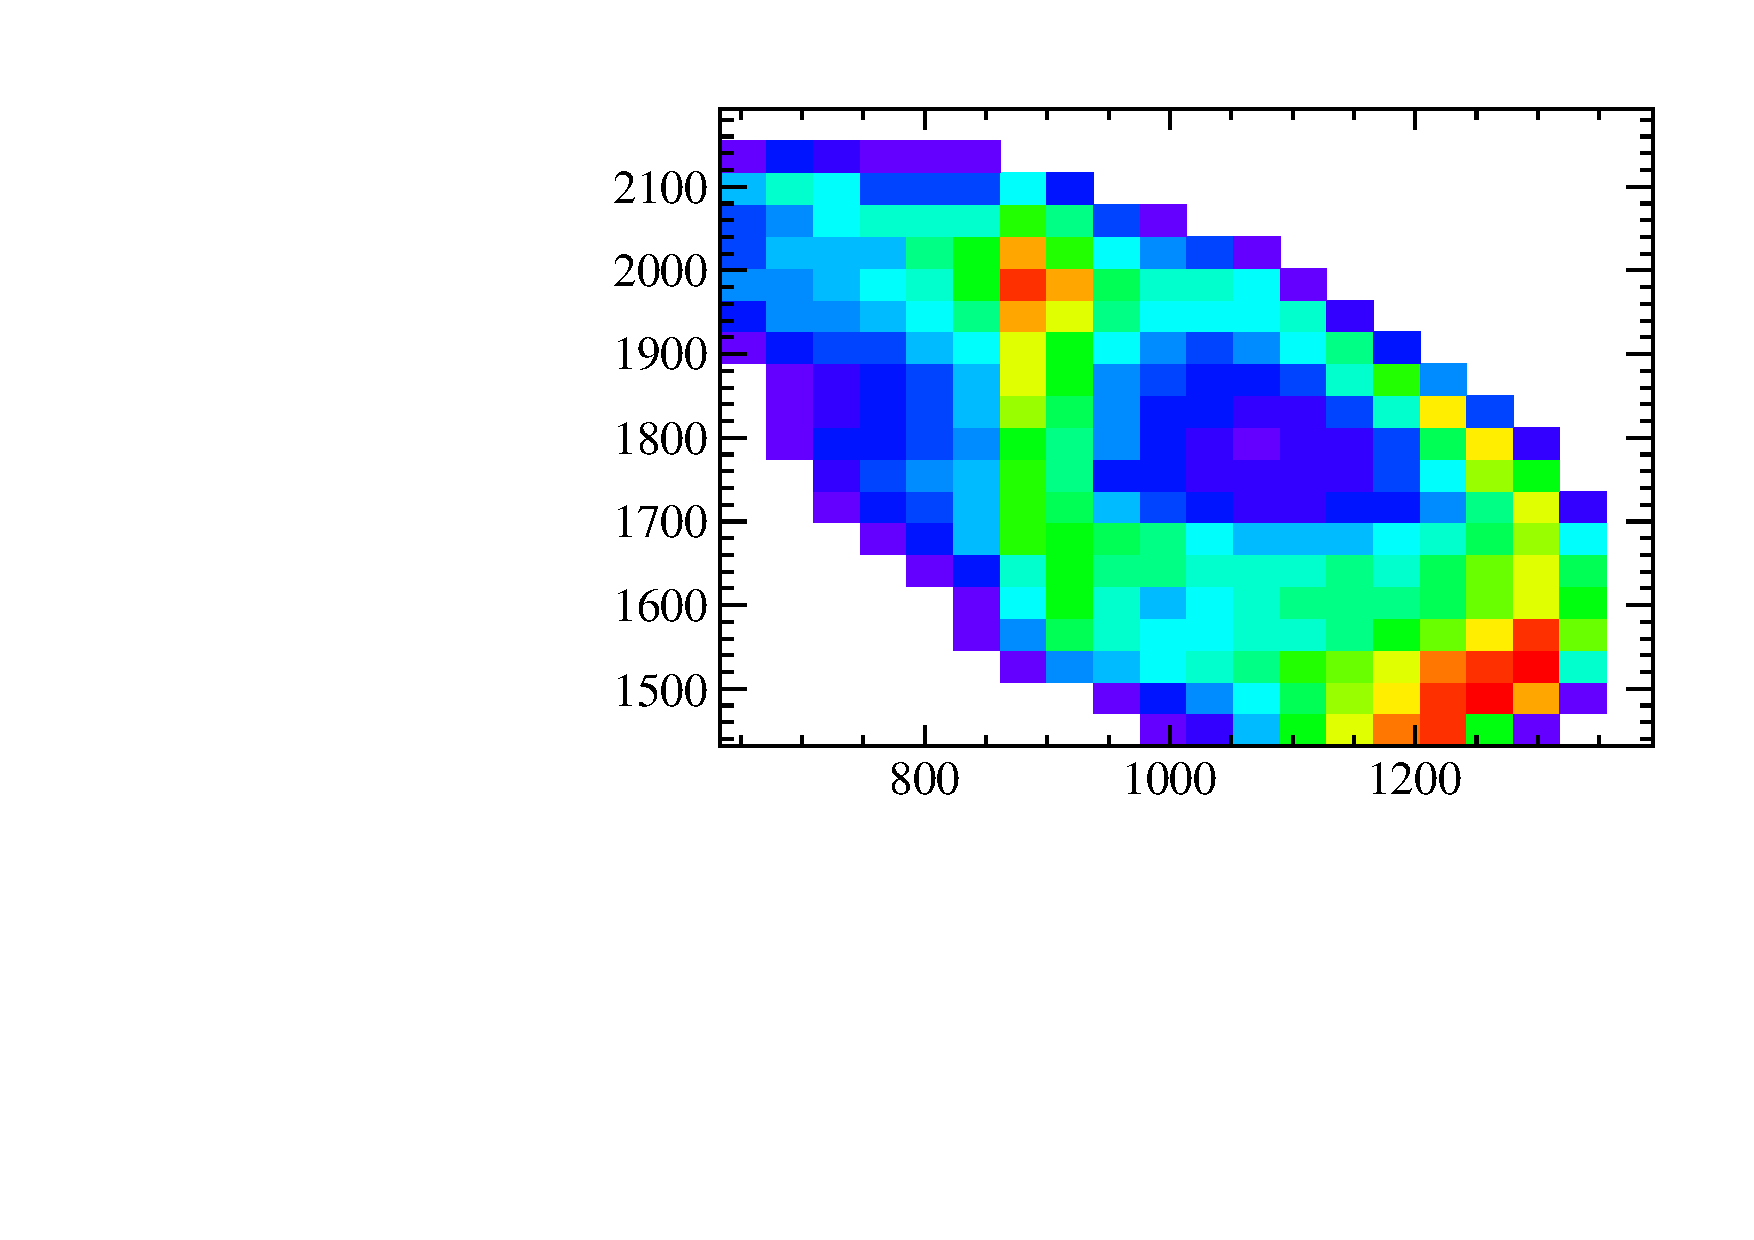
\includegraphics[width=0.45\linewidth]{plots/Lc_comparison/Lc_dalitz_data1}\put(-40,140){(e)}
    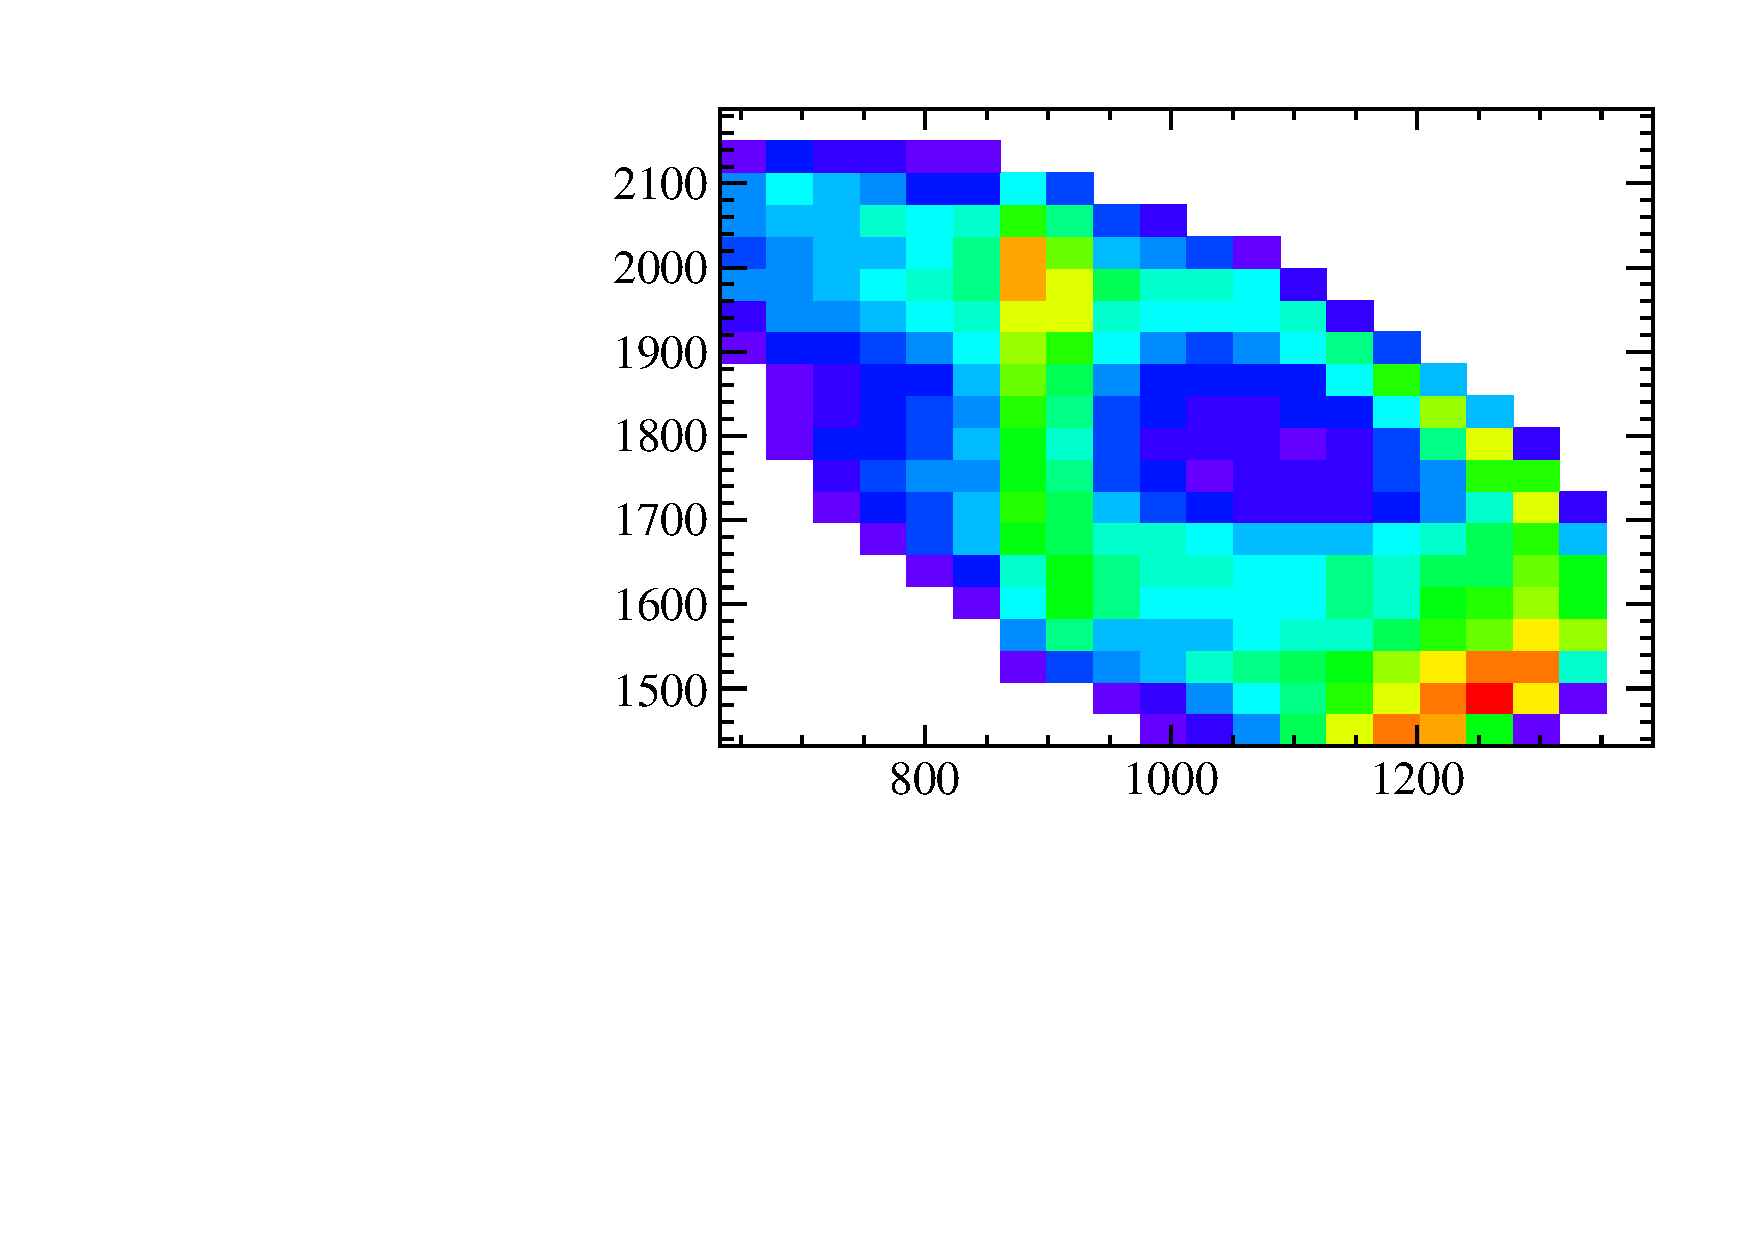
\includegraphics[width=0.45\linewidth]{plots/Lc_comparison/Lc_dalitz_data2}\put(-40,140){(f)}
    \vspace*{-0.5cm}
    \caption{\small
    Distributions of Dalitz plots for orignal MC (top),
    corrected MC (middle) and sWeighted data (bottom) in (left) forward and (right) backward regions. }
    \label{fig:dalitz}
\end{figure}
\subsection{Geometrical acceptance efficiency}
The \effacc is given by Equation \ref{eqn:acc}
\begin{equation*}\label{eqn:acc}
    \varepsilon_{\mathrm{acc}}\equiv \frac{\Lc \text{ with } \proton\Km\pip\text{ in LHCb acceptance }}{\text{Generated } \Lc}.
\end{equation*}
%The \lhcb detector covers a polar angle of $[10,400]\mrad$ with respect to the beam direction.
In this equation the acceptance refers to a range of polar angle $\theta$ of $[10,400]\mrad$ with respect to the beam direction.
So a generator-level simulation sample without geometrical acceptance requirement
is used to measure \effacc for both forward and backward rapidities.
The \effacc as a function of \pt and $y^*$ for is shown in Fig. \ref{fig:eff_geo}.
The results are summarized in Table \ref{tab:eff_acc1} and \ref{tab:eff_acc2} in Appendix \ref{app:efficiency}.
\begin{figure}[htbp]
    \begin{center}
        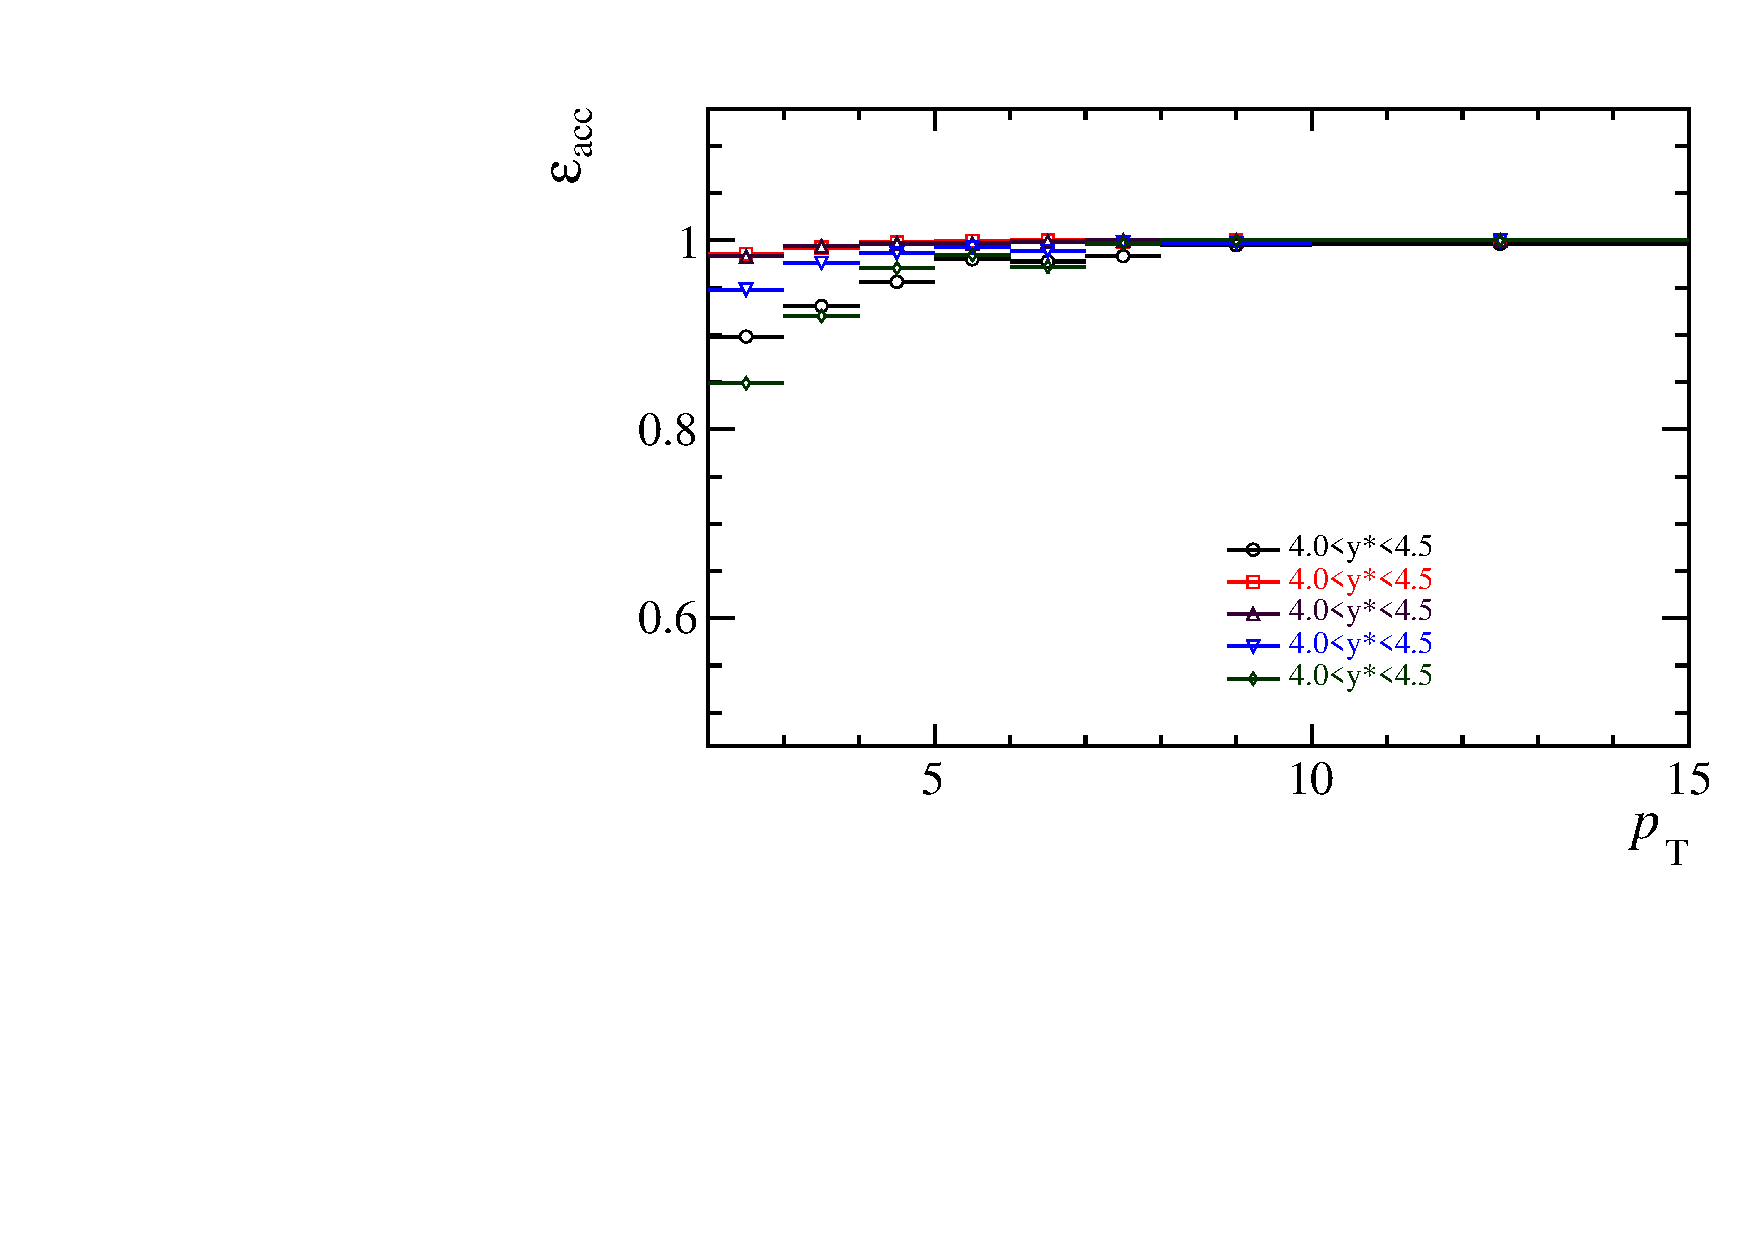
\includegraphics[width=0.45\linewidth]{plots/Lc_Acc1}\put(-40,140){(a)}
        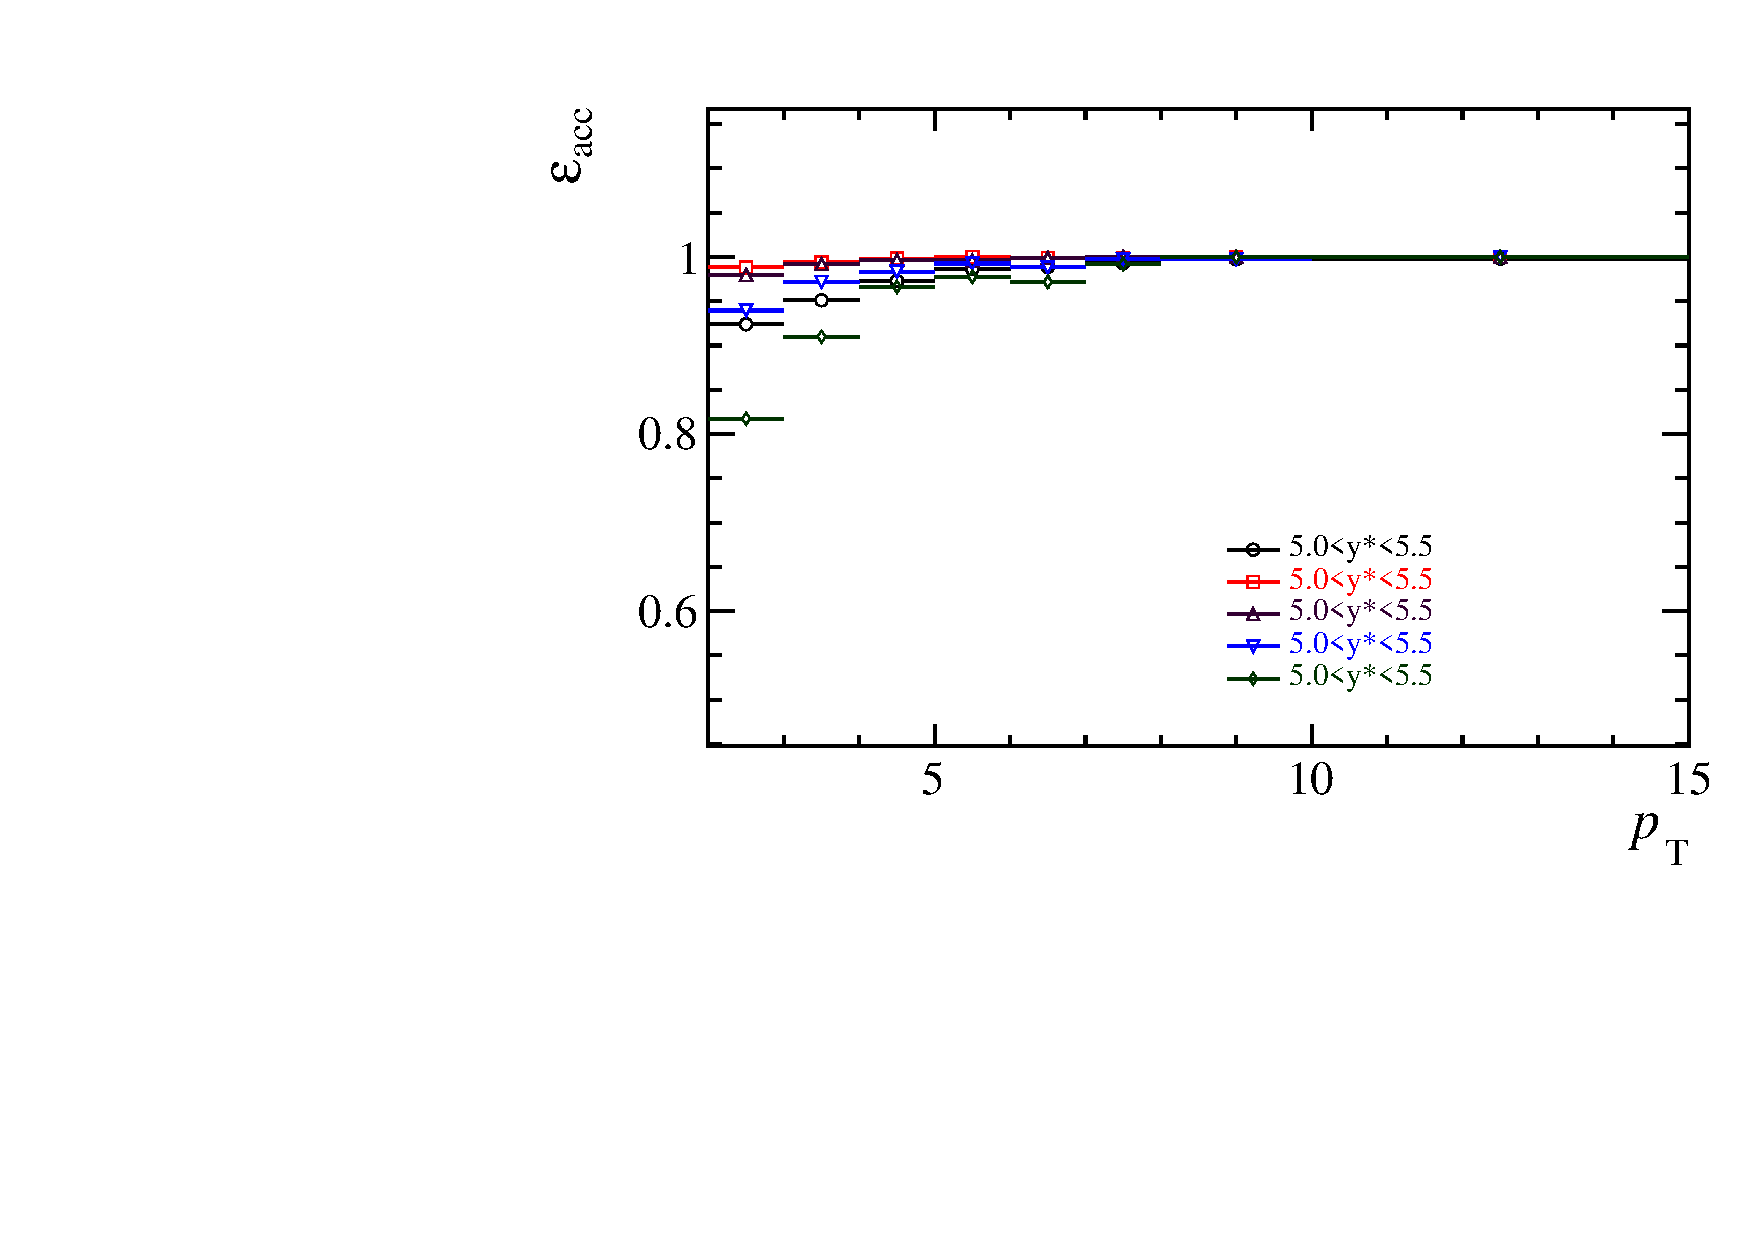
\includegraphics[width=0.45\linewidth]{plots/Lc_Acc2}\put(-40,140){(b)}
        \vspace*{-0.5cm}
    \end{center}
    \caption{\small
    The geometrical acceptance efficiency \effacc as a function of \pt and $y^*$ of prompt \Lc baryon
    for (left) forward and (right) backward rapidities. Statistical uncertainties only.}
    \label{fig:eff_geo}
\end{figure}

\subsection{Reconstruction and selection efficiency}
The reconstruction and selection efficiency is defined as
\begin{equation}\label{eqn:recandsel}
    \varepsilon_{\mathrm{rec\&sel}}= \frac{\sum \Lc \text{in acceptance, reconstructed and selected}}
    {\Lc\text{ with }\proton\Km\pip \text{ in LHCb acceptance}}~.
\end{equation}
This efficiency include two parts: the efficiency of reconstructing the three long tracks
and the refinement of the \Lc signals.
The selections are listed in Tables~\ref{tab:HLT2} and~\ref{tab:offline} without PID requirements.
As the HLT1 selections for tracks in Table~\ref{tab:HLT1} are also cut-based,
so they are also included in this section.
The sample for calculating this efficiency is truth matched $\decay{\Lc}{\proton\Km\pip}$ decays
in \plead full simulation sample.
The {\it truth matching} requires that
particle IDs are in agreement with there PDG IDs and
the background category ({\tt BKGCAT}) equals to 0 (signal) or 50 (low-mass background).
There are two extra corrections to be considered in \effsel calculation,
which are truth matching inefficiency and track finding efficiency.

\subsubsection{Truth matching inefficiency}
The signals in the simulation are picked out by truth matching requirements,
but the truth matching algorithm occasionally flags the signal track as a ghost.
This effect can be seen by plotting the $M(\proton\Km\pip)$ distribution of not truth matched passing the selections.
A peak around \Lc mass can be seen from the blue points in Fig.~\ref{fig:truth_match}.
The ratio of the number of \Lc signal in this peak over the total number (truth matched) of \Lc signal.
A Gaussian signal plus a linear background is used to fit the mass spectrum.
The fits give a global fraction of $0.01\%$ for both rapidities.
The effect would result in an underestimate of the efficiency,
thus the total efficiency should be multiplied by a factor of 1.0001 for Fwd and 1.0001 for Bwd.
As the fraction is quite small, uncertainties and kinematic dependence are also negligible.
\begin{figure}[htbp]
    \begin{center}
        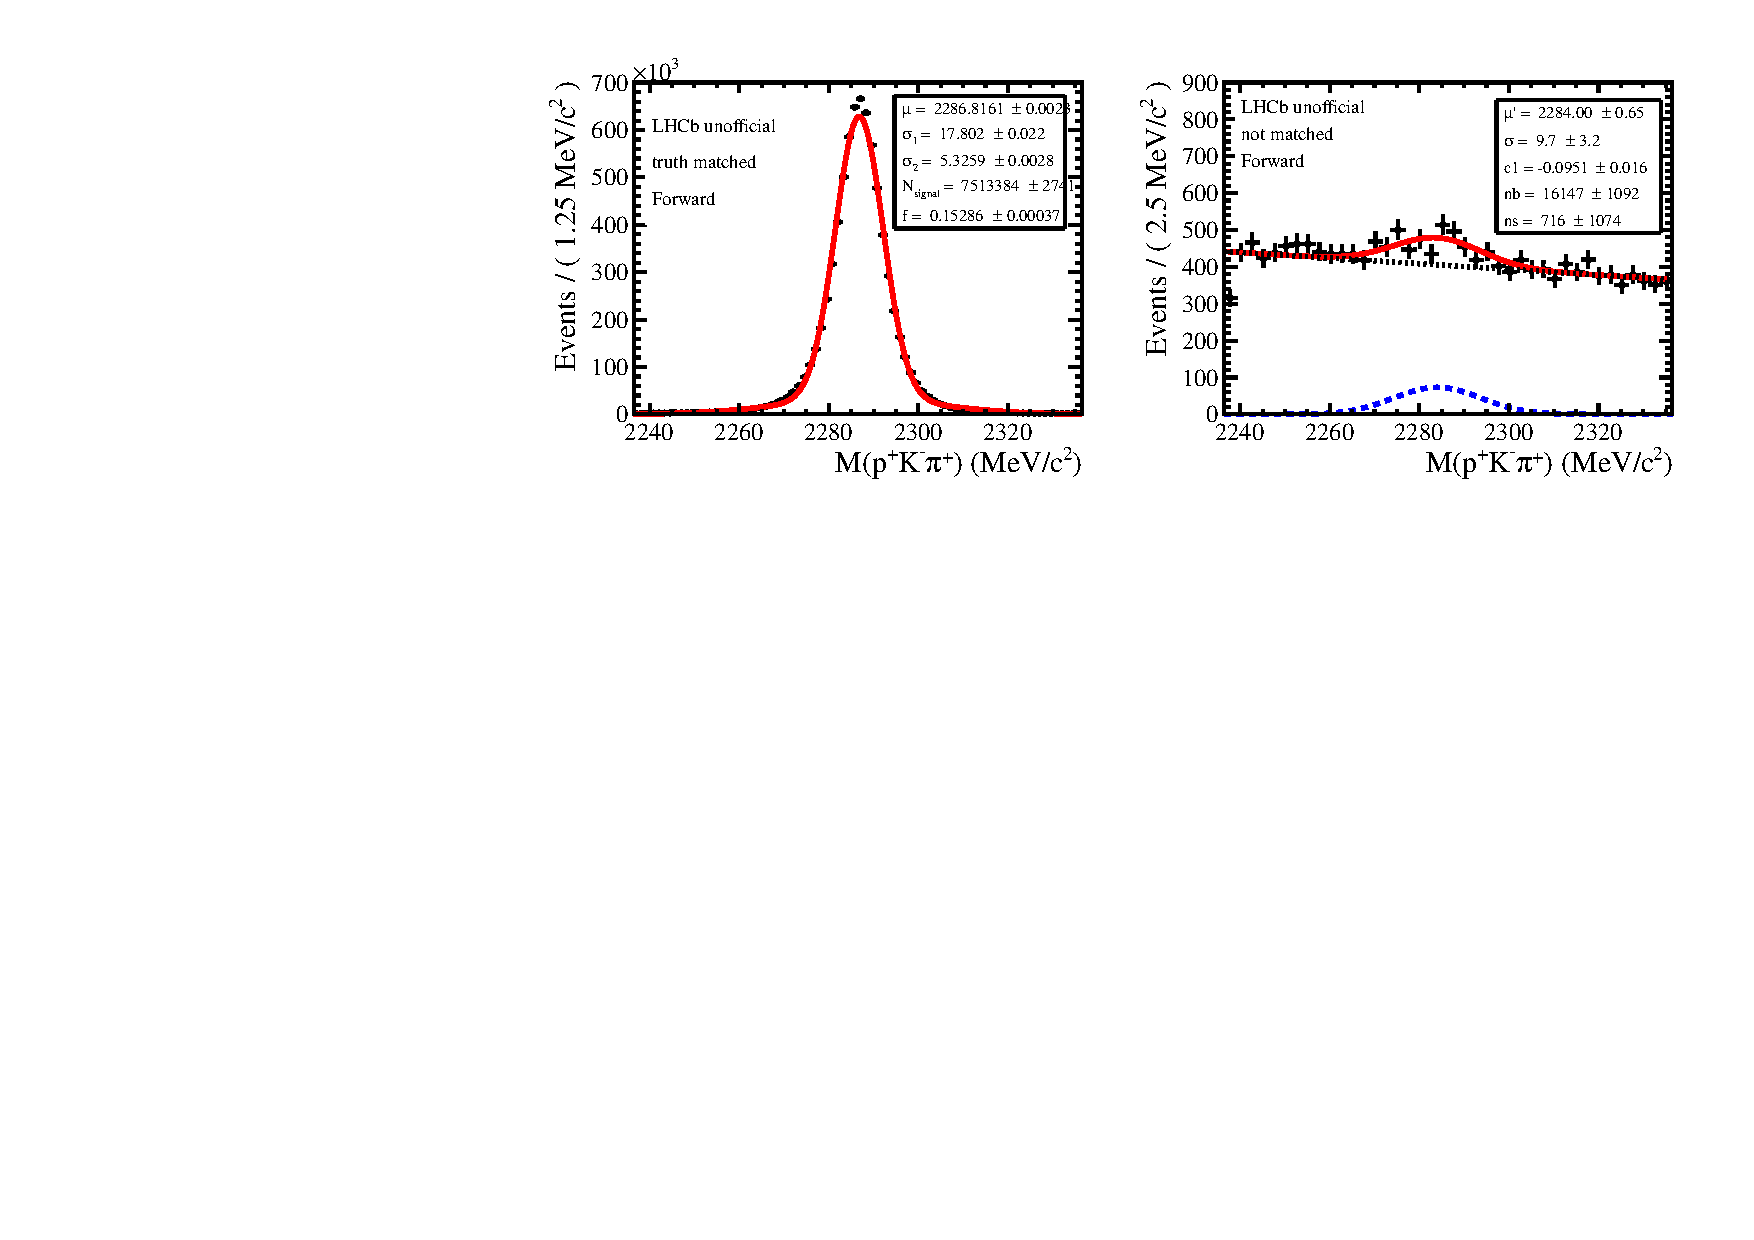
\includegraphics[width=0.9\linewidth]{fit_pA}\put(-250,150){(a)}\put(-40,150){(b)}

        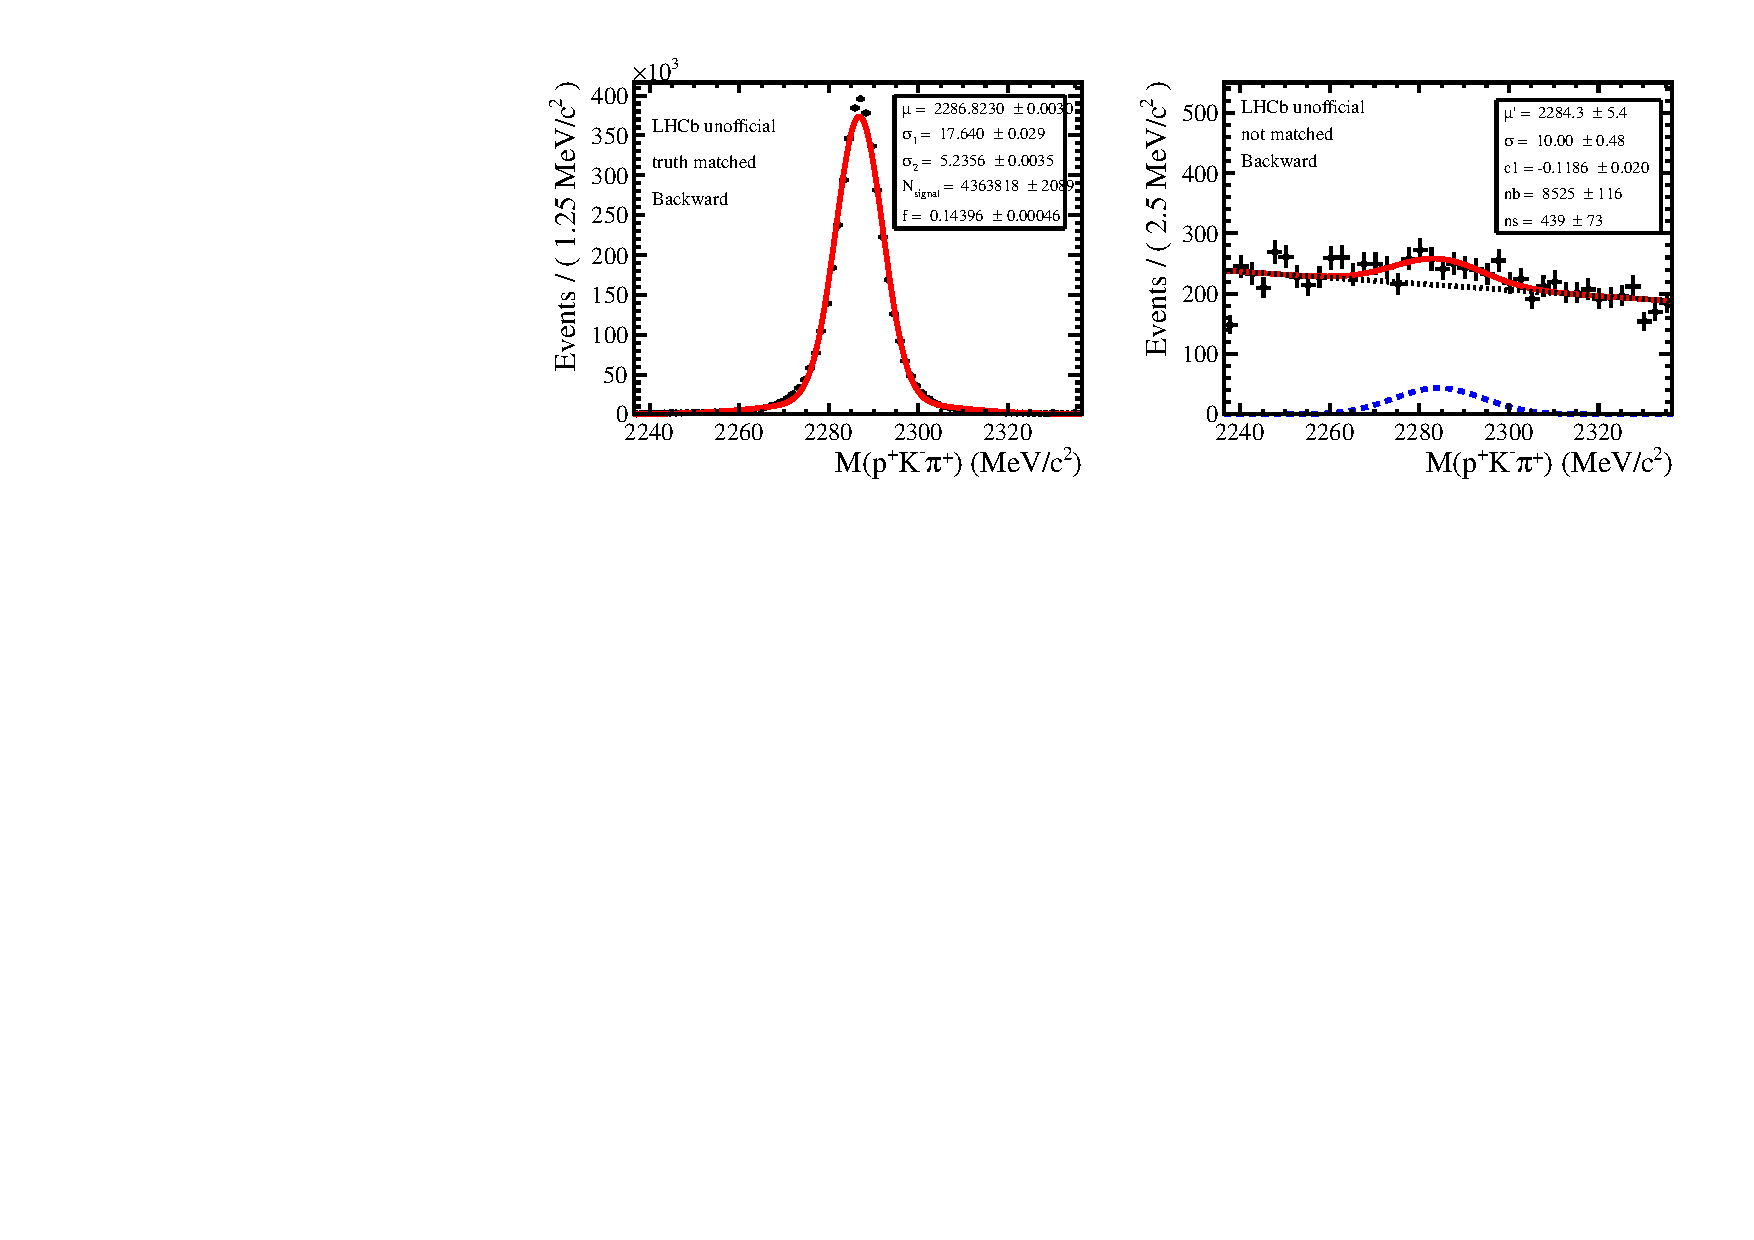
\includegraphics[width=0.9\linewidth]{fit_Ap}\put(-250,150){(c)}\put(-40,150){(d)}
        \vspace*{-0.5cm}
    \end{center}
    \caption{\small
    The $M(\kaon\pion)$ distribution of (left) truth matched and (right) not matched \Lc baryons
    for (top) foward and (bottom) backward simulations.}
    \label{fig:truth_match}
\end{figure}

\subsubsection{Tracking correction}
The track finding efficiency for data and simulation is different.
Calibrations are performed using a tag-and-probe method~\cite{LHCb-PUB-2011-025},
with $\decay{\jpsi}{\mup\mun}$ and $\decay{\KS}{\pip\pim}$ decays.
The tables are the same as that from the \Lc production in $p$Pb
at $\sqsnn=8.16\tev$~\cite{LHCb-PAPER-2022-007}(LHCb-ANA-2019-039),
given in histograms of track momemtum $p$ and pseudo-rapidity $\eta$.
When performing this correction, the weights are applied to selected candidates only,
defined as
\begin{equation}\label{eqn:tracking}
    \varepsilon_{\mathrm{rec\&sel}}= \frac{\sum_{\Lc \text{reconstructed and selected}}
    w_i(p_\proton, \eta_\proton)\times w_i(p_{\Km},\eta_{\Km})\times w_i(p_{\pip},\eta_{\pip})}
    {\Lc\text{ with }\proton\Km\pip \text{ in LHCb acceptance}}~.
\end{equation}
\begin{figure}[htbp]
    \begin{center}
        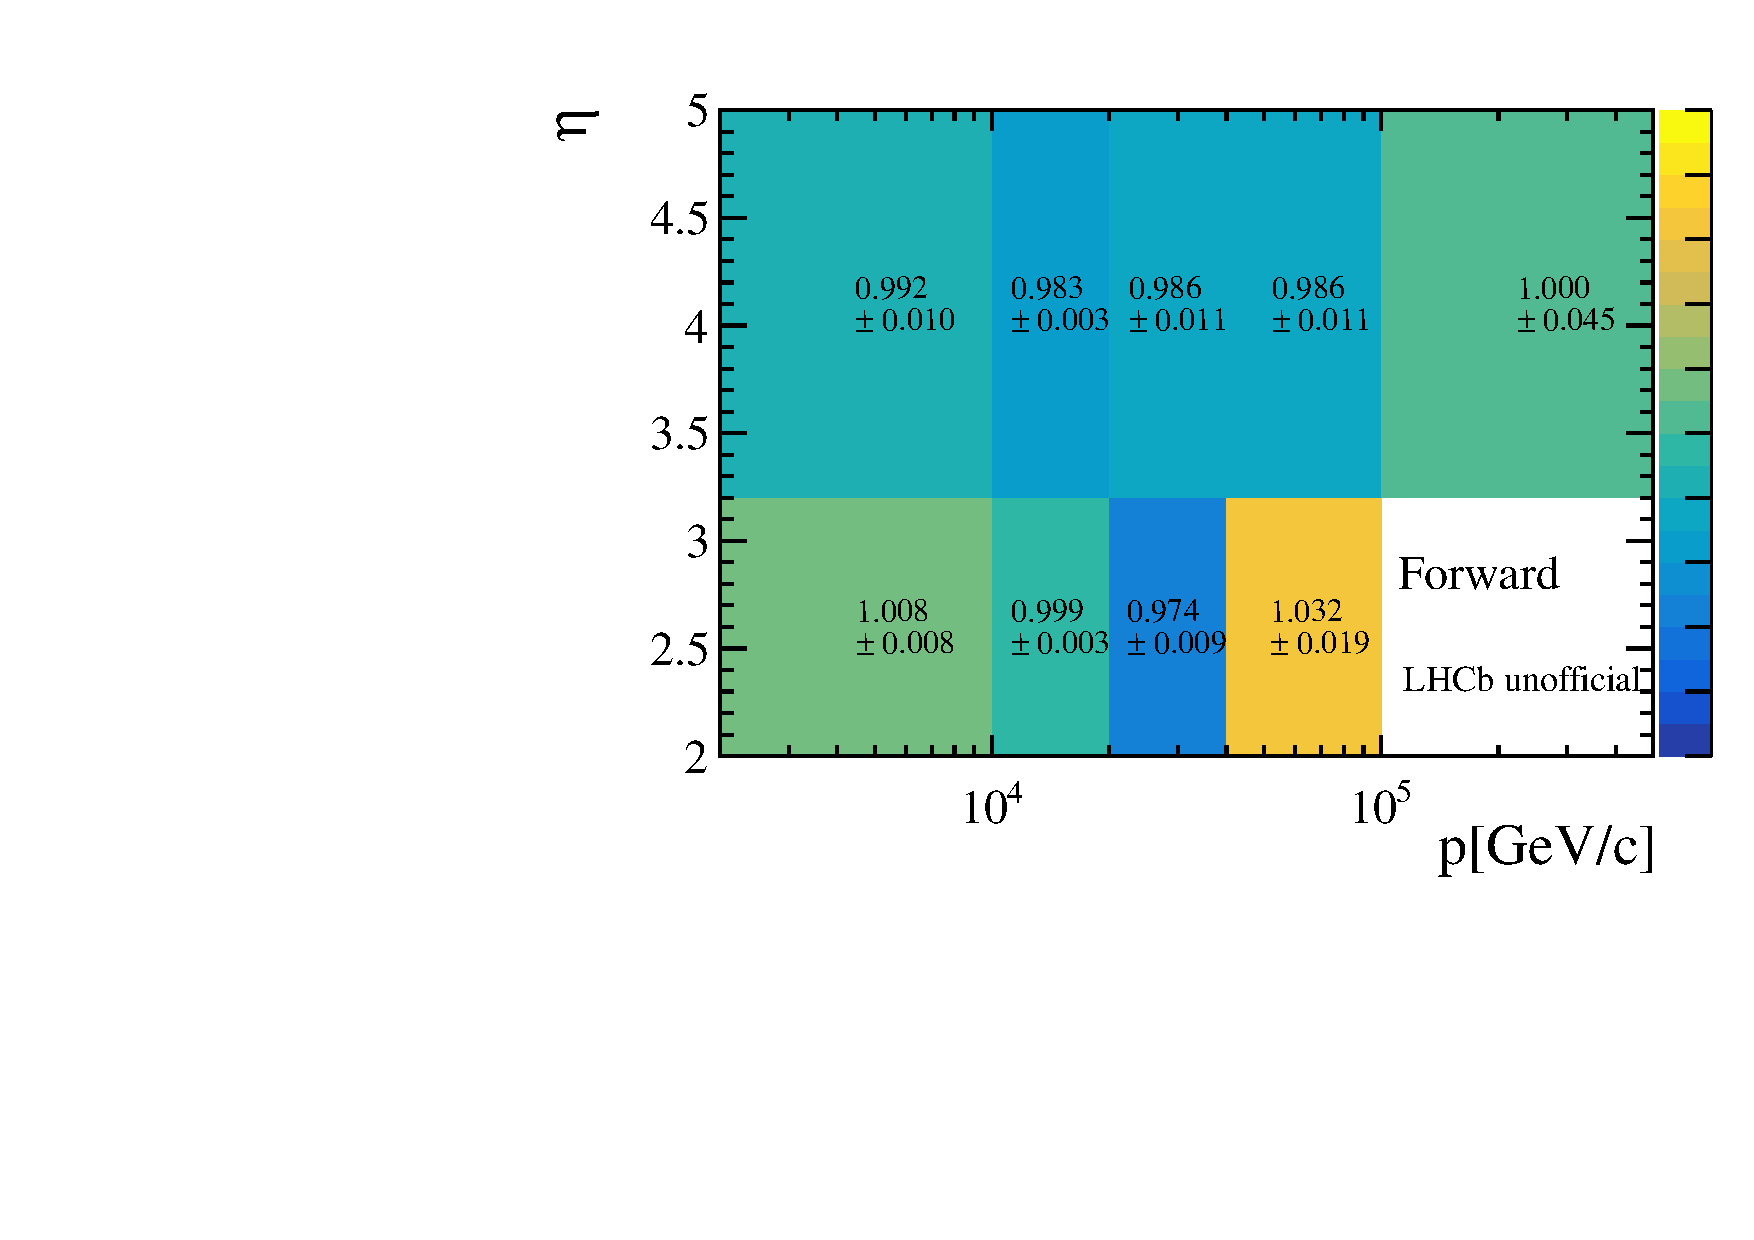
\includegraphics[width=0.45\linewidth]{tracking_table_pA}\put(-40,140){(a)}
        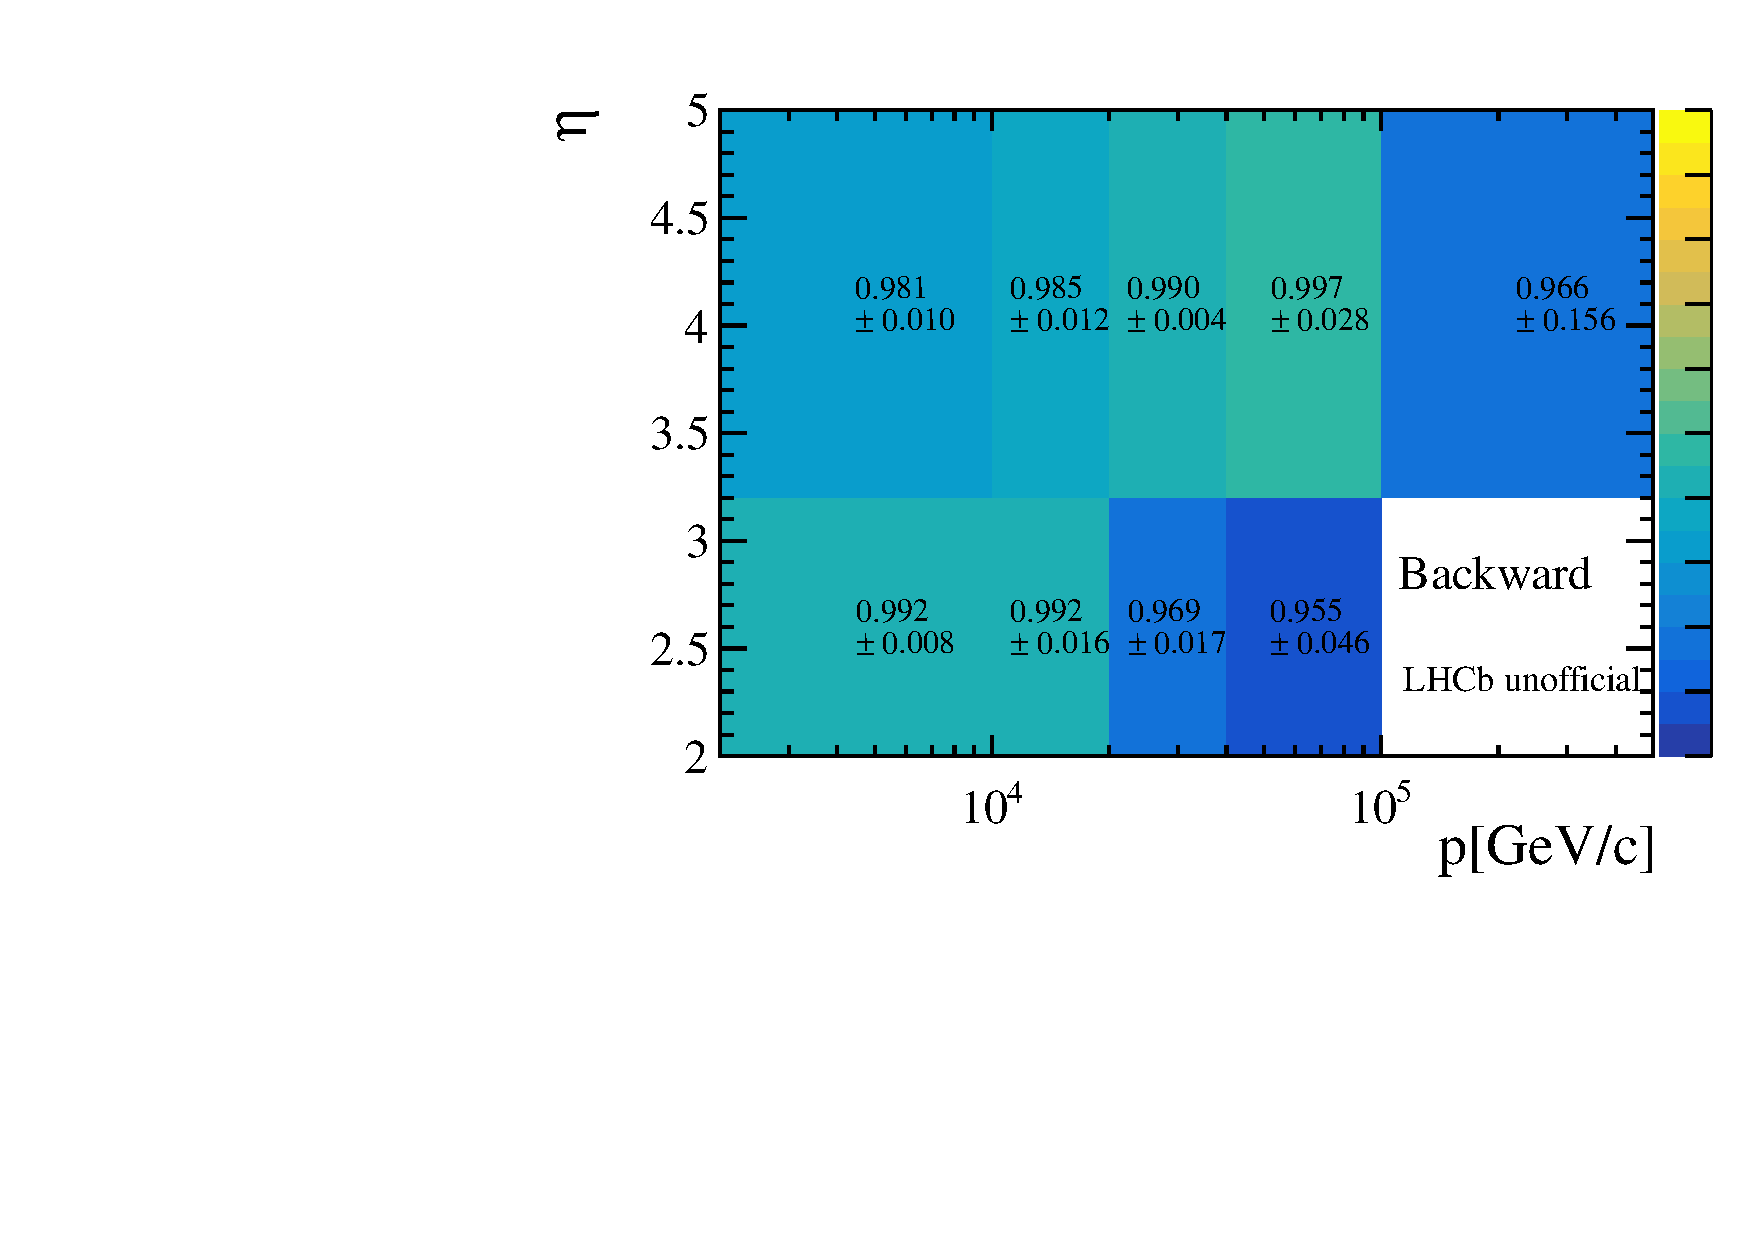
\includegraphics[width=0.45\linewidth]{tracking_table_Ap}\put(-40,140){(b)}
        \vspace*{-0.5cm}
    \end{center}
    \caption{\small
    Tracking calibration table of (left) forward and (right) backward rapidities.}
    \label{fig:tracking}
\end{figure}

shown in Fig. \ref{fig:eff_sel} and incorporated with all corrections.
The numerical values are listed in the Table \ref{tab:eff_sel1} and \ref{tab:eff_sel2}.
\begin{figure}[htbp]
    \begin{center}
        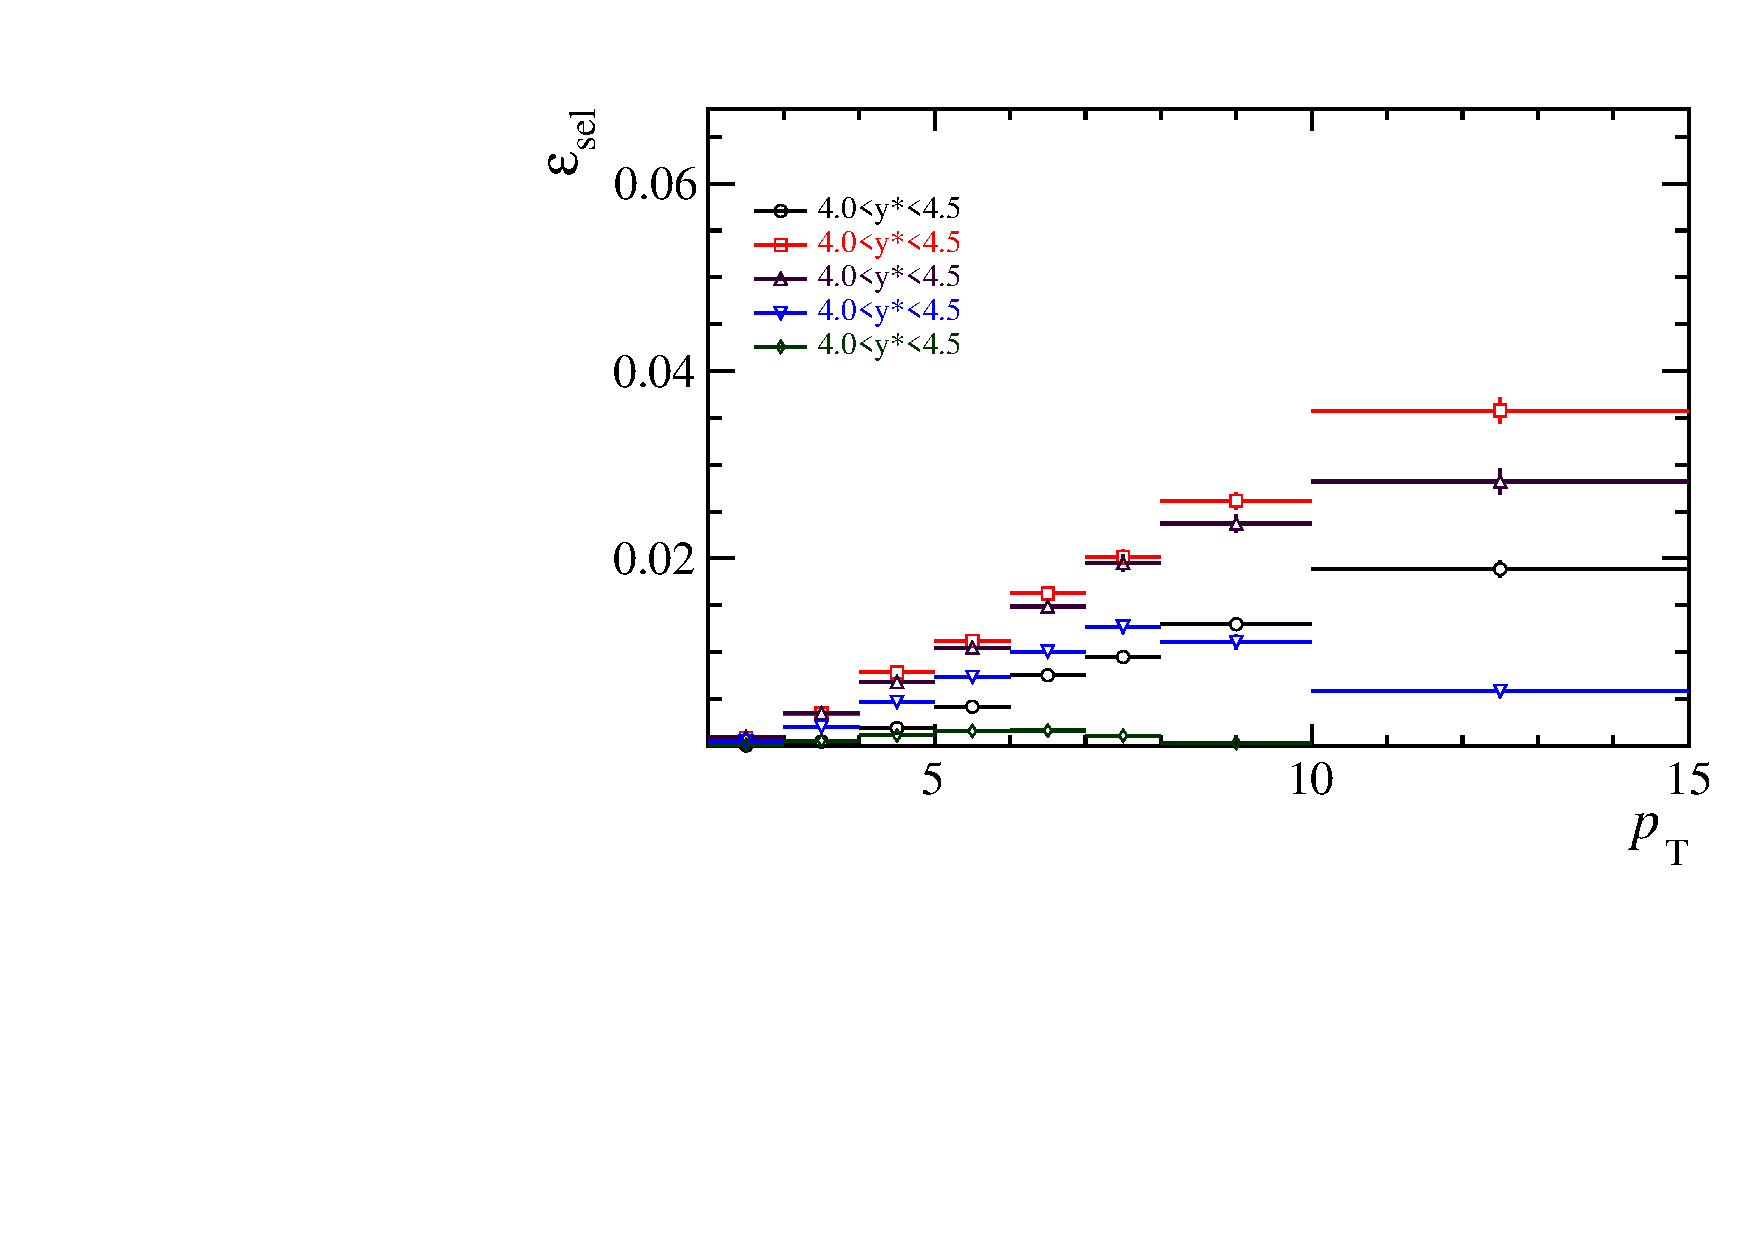
\includegraphics[width=0.45\linewidth]{plots/Lc_Sel1}\put(-40,140){(a)}
        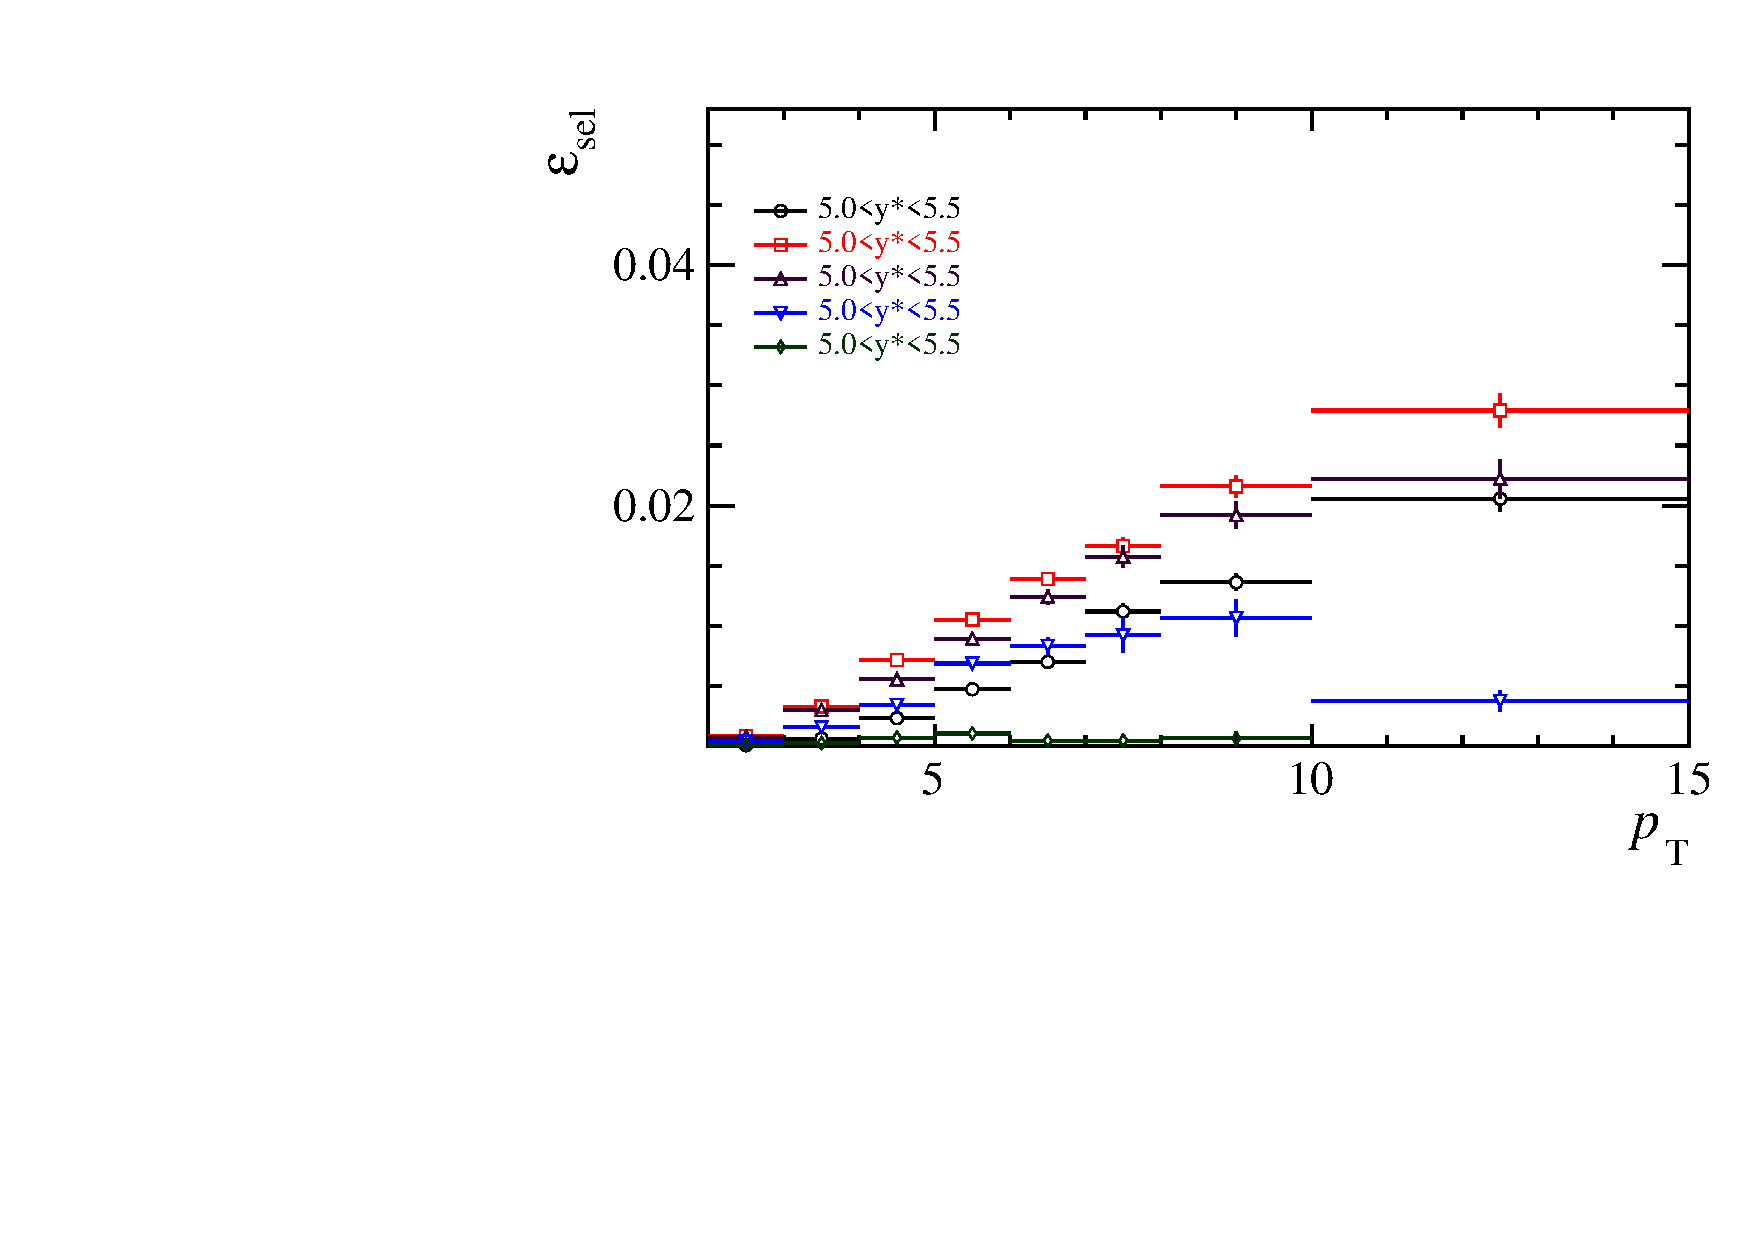
\includegraphics[width=0.45\linewidth]{plots/Lc_Sel2}\put(-40,140){(b)}
        \vspace*{-0.5cm}
    \end{center}
    \caption{\small
    The selection efficiency $\varepsilon_\mathrm{rec\&sel}$~ as a function of \pt and $y^*$ of prompt \Lc baryon
    for Fwd (top) and Bwd (bottom) configurations with all corrections considered.
    Statistical uncertainties only.}
    \label{fig:eff_sel}
\end{figure}

\subsection{PID efficiency}
The \effpid of \Lc particle is evaluated with single track PID efficiencies
with the formula
\begin{equation}\label{eqn:eff_pid}
    \varepsilon_{\mathrm{PID}}\equiv
    \frac{\sum_i^N \varepsilon_{\proton} \times\varepsilon_{\kaon} \times\varepsilon_{\pion}}
    {\sum_i^N \Lc~\text{reconstructed and selected}}~,
\end{equation}
where the sum goes over the selected \Lc simulation candidates.
In Table \ref{tab:HLT2} and \ref{tab:offline},
the selections are $\mathrm{DLL}_{\proton\pion}(\proton)>15$
and $\mathrm{DLL}_{\proton\kaon}(\proton)>5$.
and $\mathrm{DLL}_{\kaon\pion}(\Km)>5$.
and $\mathrm{DLL}_{\kaon\pion}(\pip)<0$.
The single track PID efficiencies 
are given as a function of $(p,\eta, \nVeloClusters)$
and are estimated with data-driven methods.
The calibration tables can be easily obtained from the package PIDCalib of \urania,
in the form of three-dimensional histograms, seeing \url{https://twiki.cern.ch/twiki/bin/view/LHCb/PIDCalibPackage}.
For the \kaon and \pion tables, the statistics are less than 150k,
which limits the bin numbers of the histogram.
Thus, the three-dimensional efficiencies can be obtained by multiplying the efficiency in different axses,
that is
\begin{equation}\label{eqn:PIDeff_3D}
    \varepsilon_\mathrm{PID}(p,\eta,\mathrm{nVeluClusters})
    = \varepsilon_\mathrm{PID}(p,\eta) \times \varepsilon(\nVeloClusters) / \overline{\varepsilon}_\mathrm{PID}~.
\end{equation}
The independence between the kinematic variables and multiplicity variables need to be examined before.
Thus, the $\nVeloClusters$ distributions in different kinematic regions
are shown in Figs.~\ref{fig:PID_K},~\ref{fig:PID_pi} and~\ref{fig:PID_p}.
This independence holds for \kaon and \pion samples,
while does not hold for \proton sample.
\begin{figure}[htbp]
    \centering
    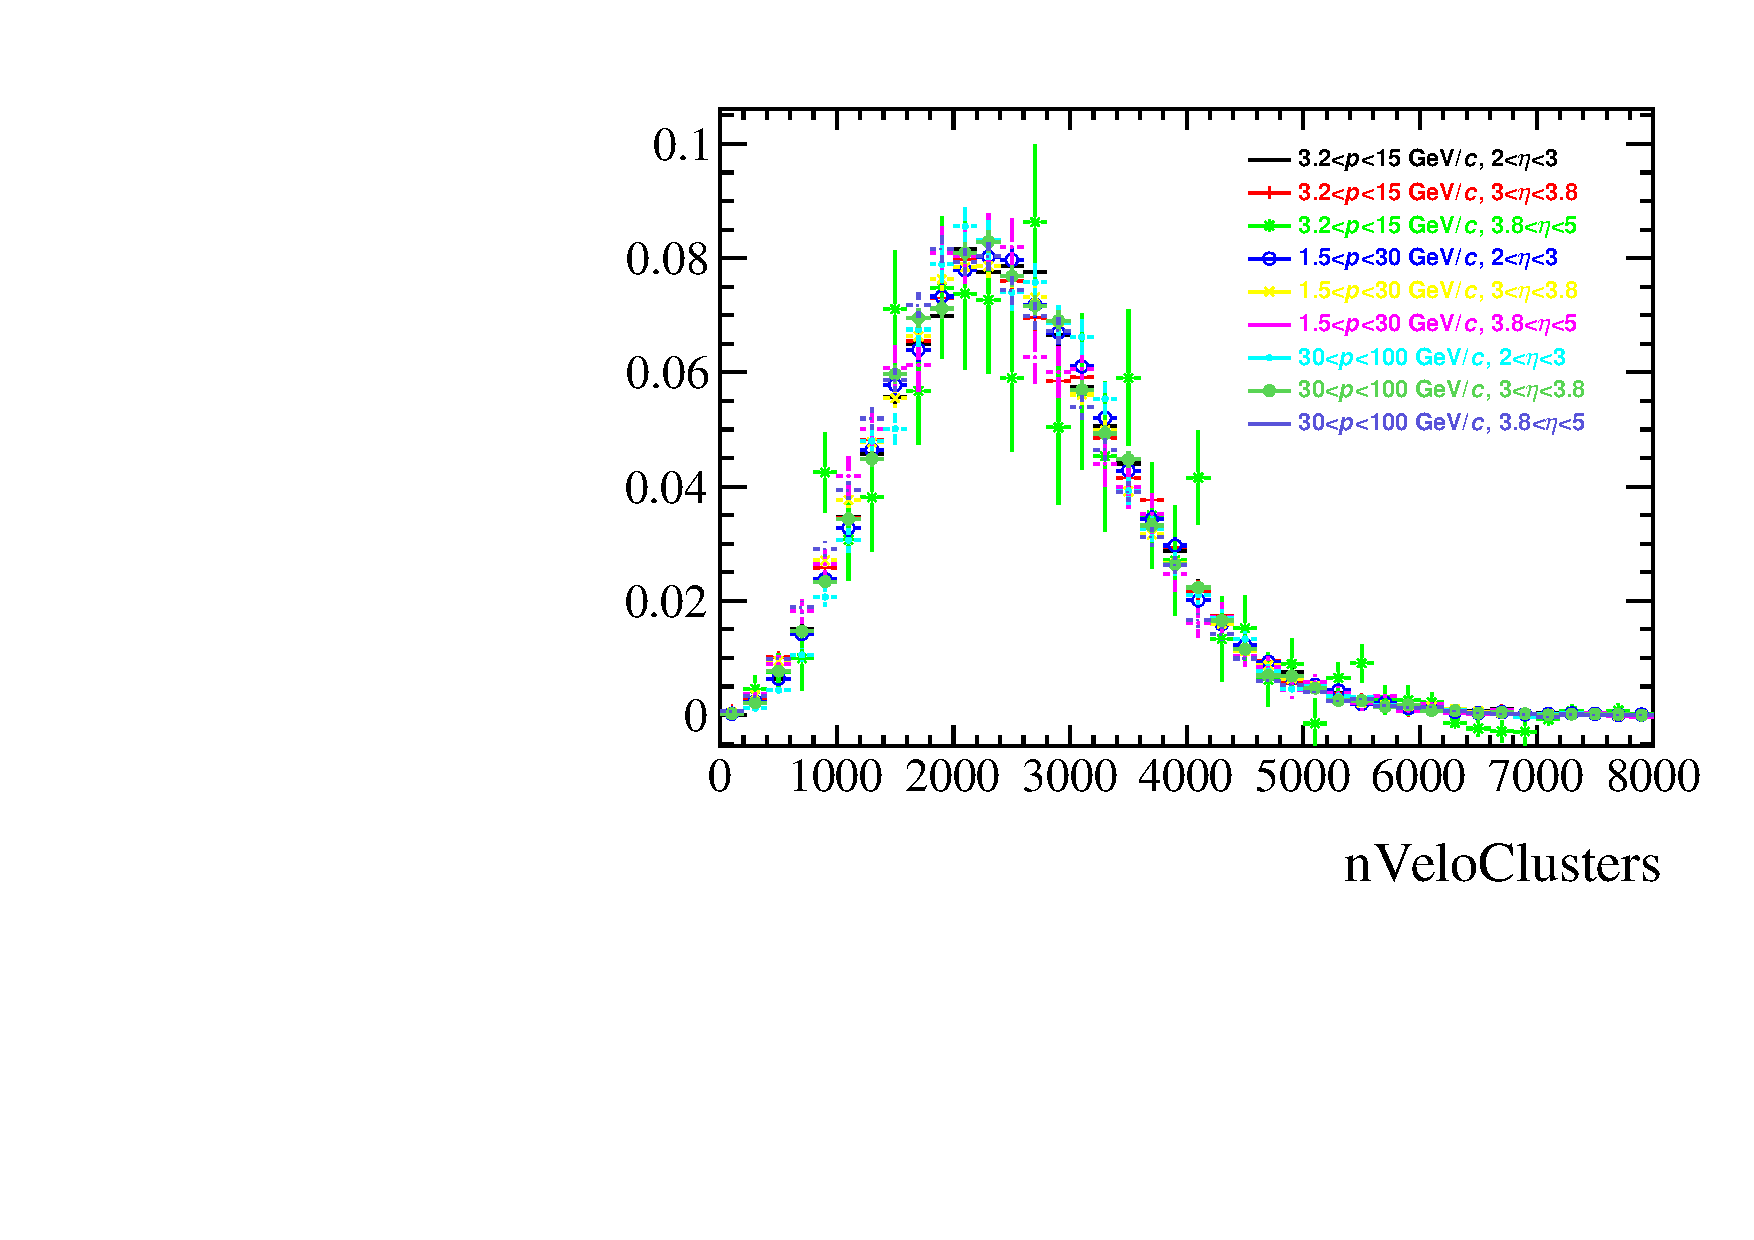
\includegraphics[width=0.45\linewidth]{PID/K_Total_pA}\put(-40,140){(a)}
    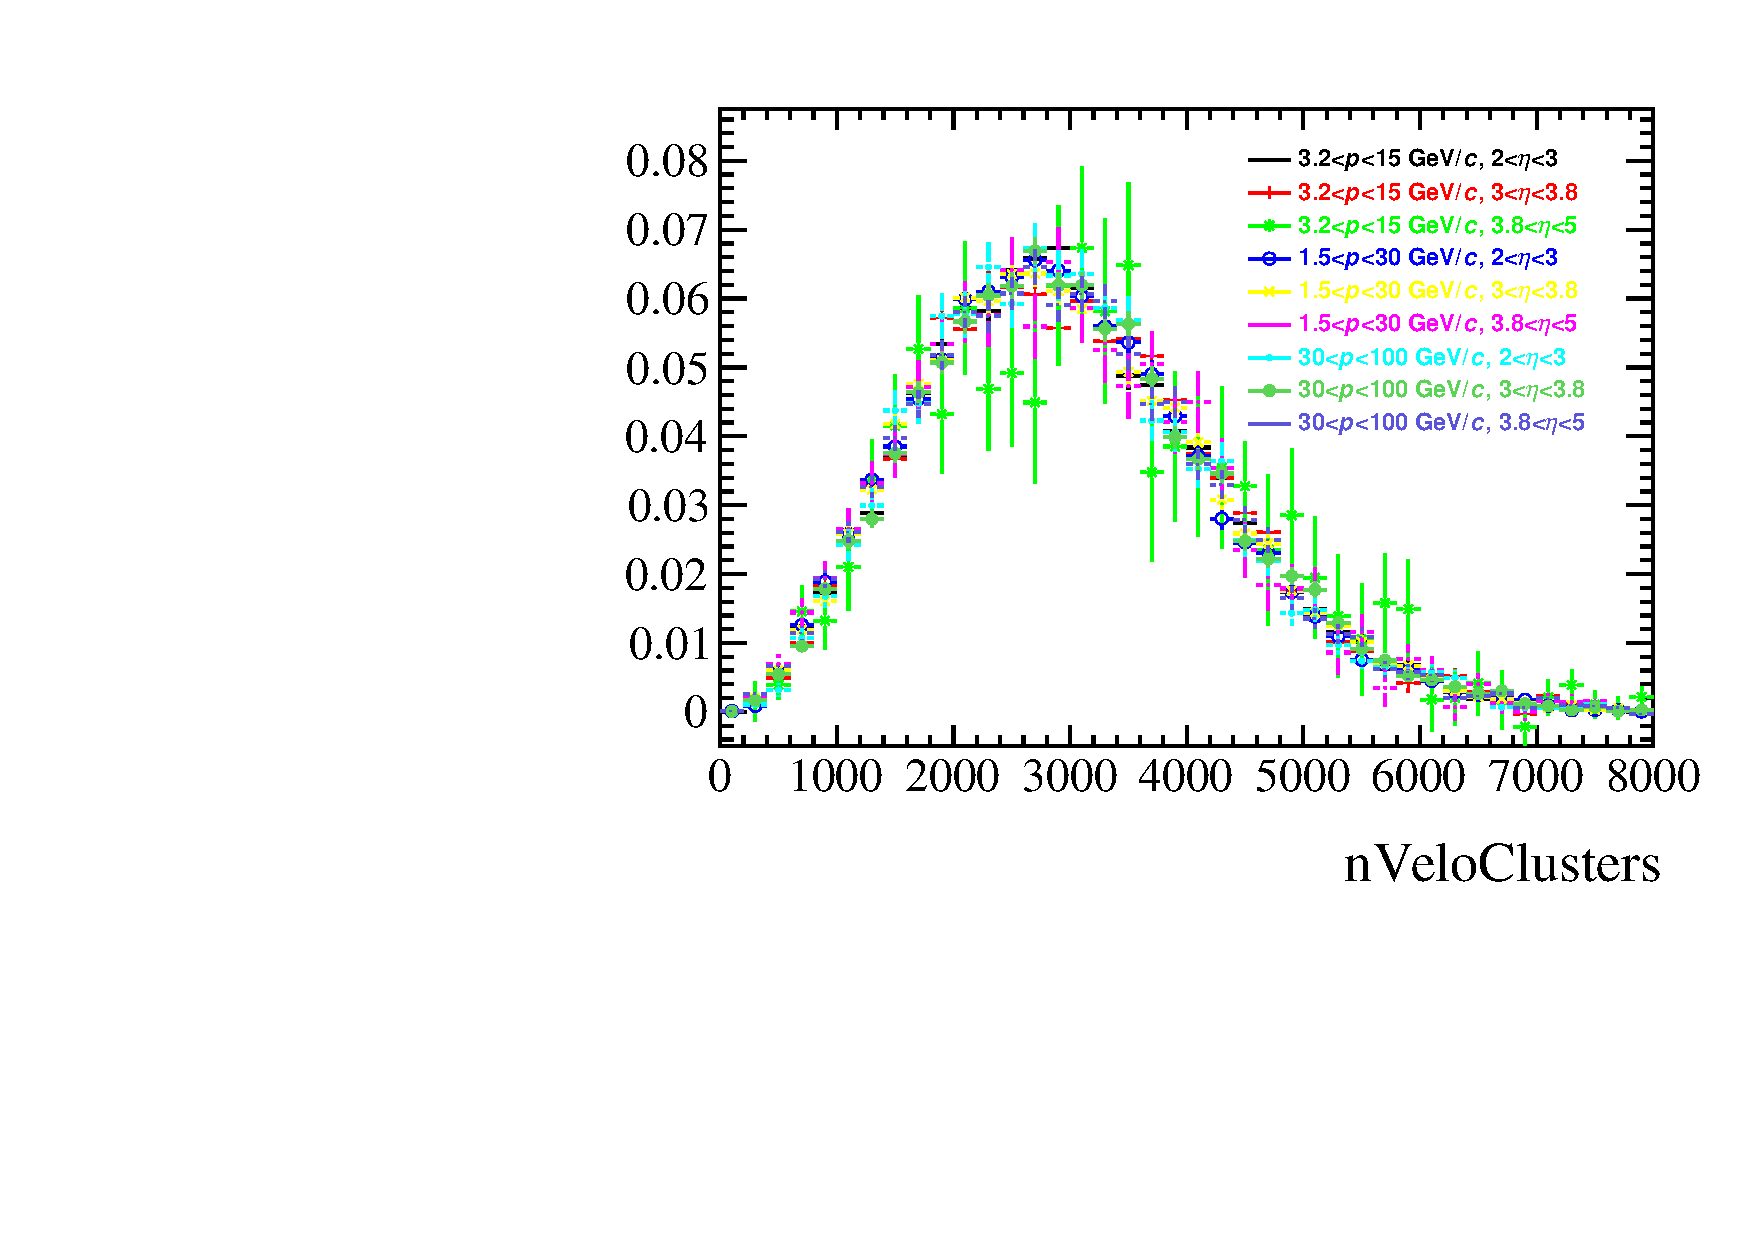
\includegraphics[width=0.45\linewidth]{PID/K_Total_Ap}\put(-40,140){(b)}

    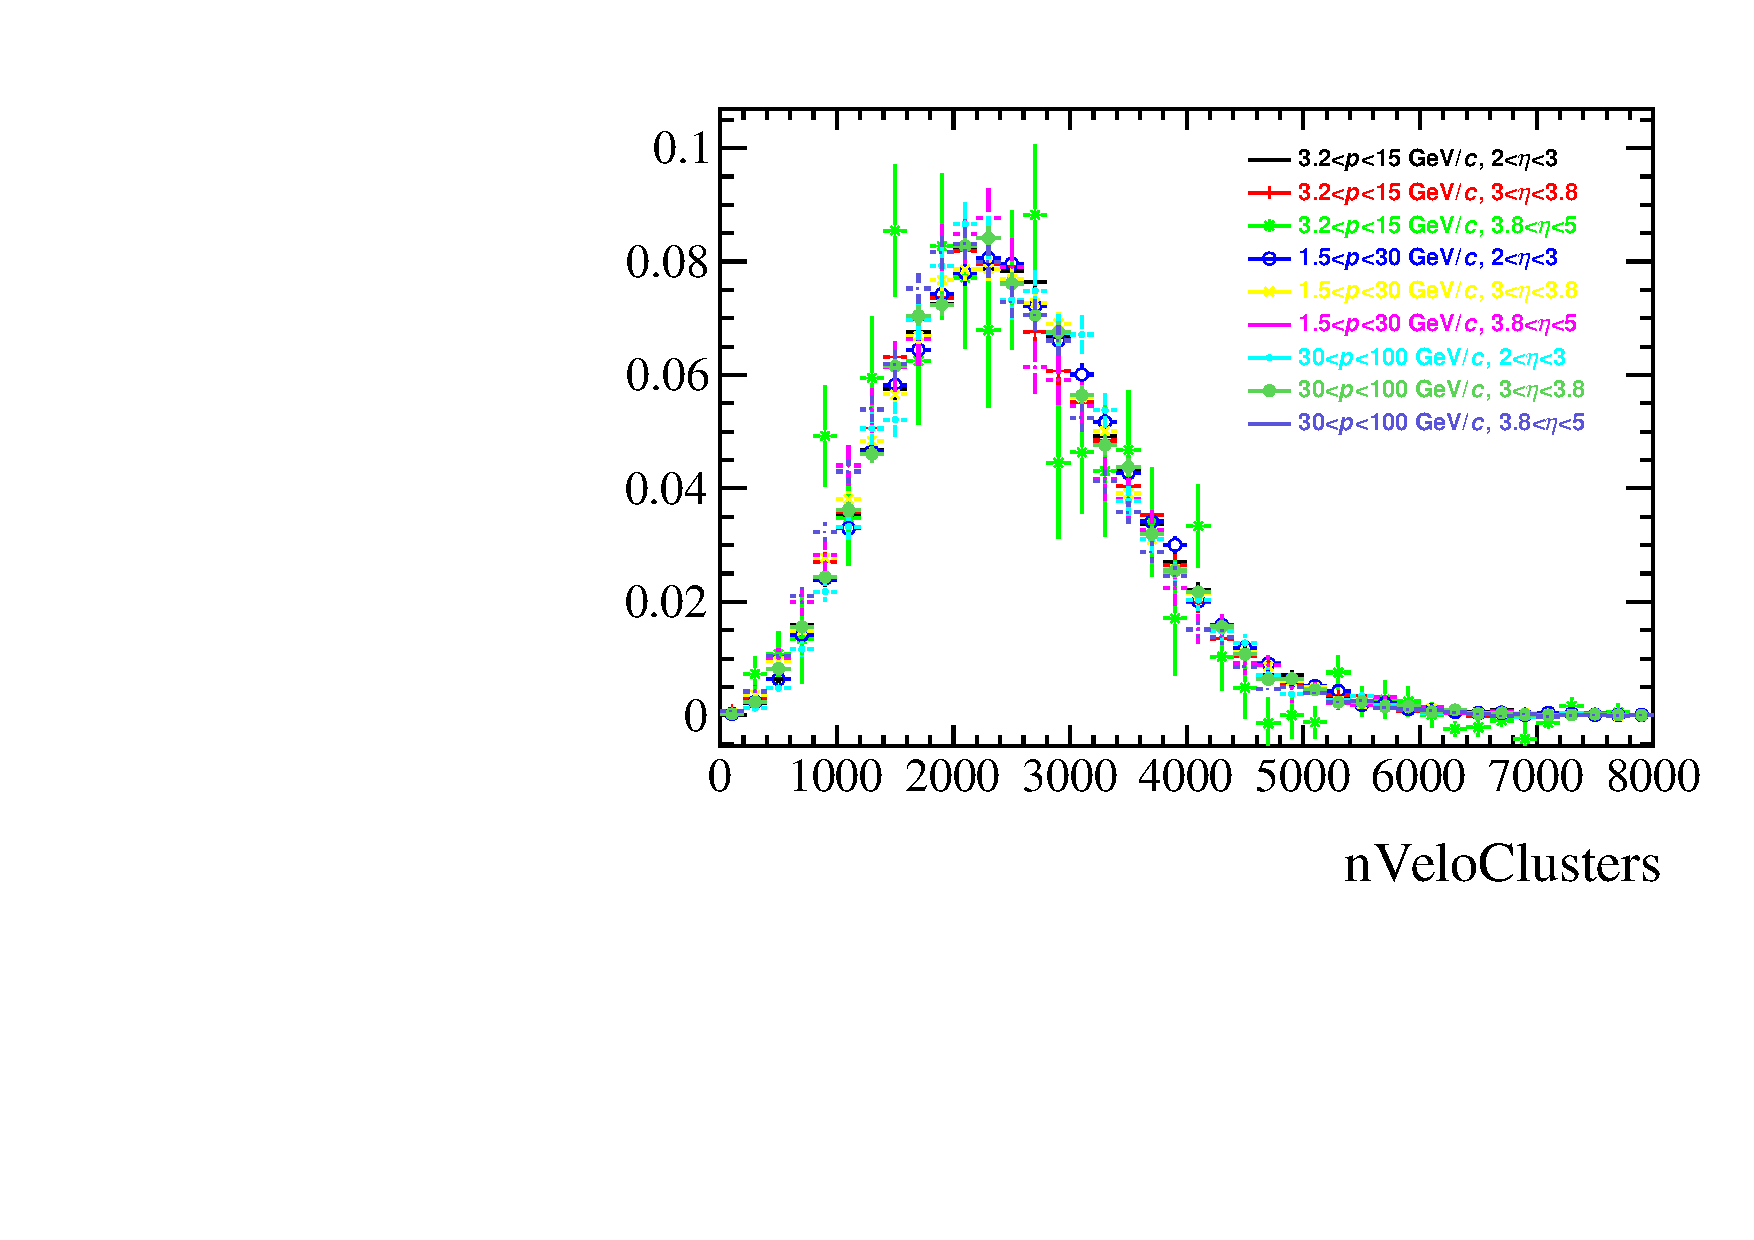
\includegraphics[width=0.45\linewidth]{PID/K_Passed_pA}\put(-40,140){(c)}
    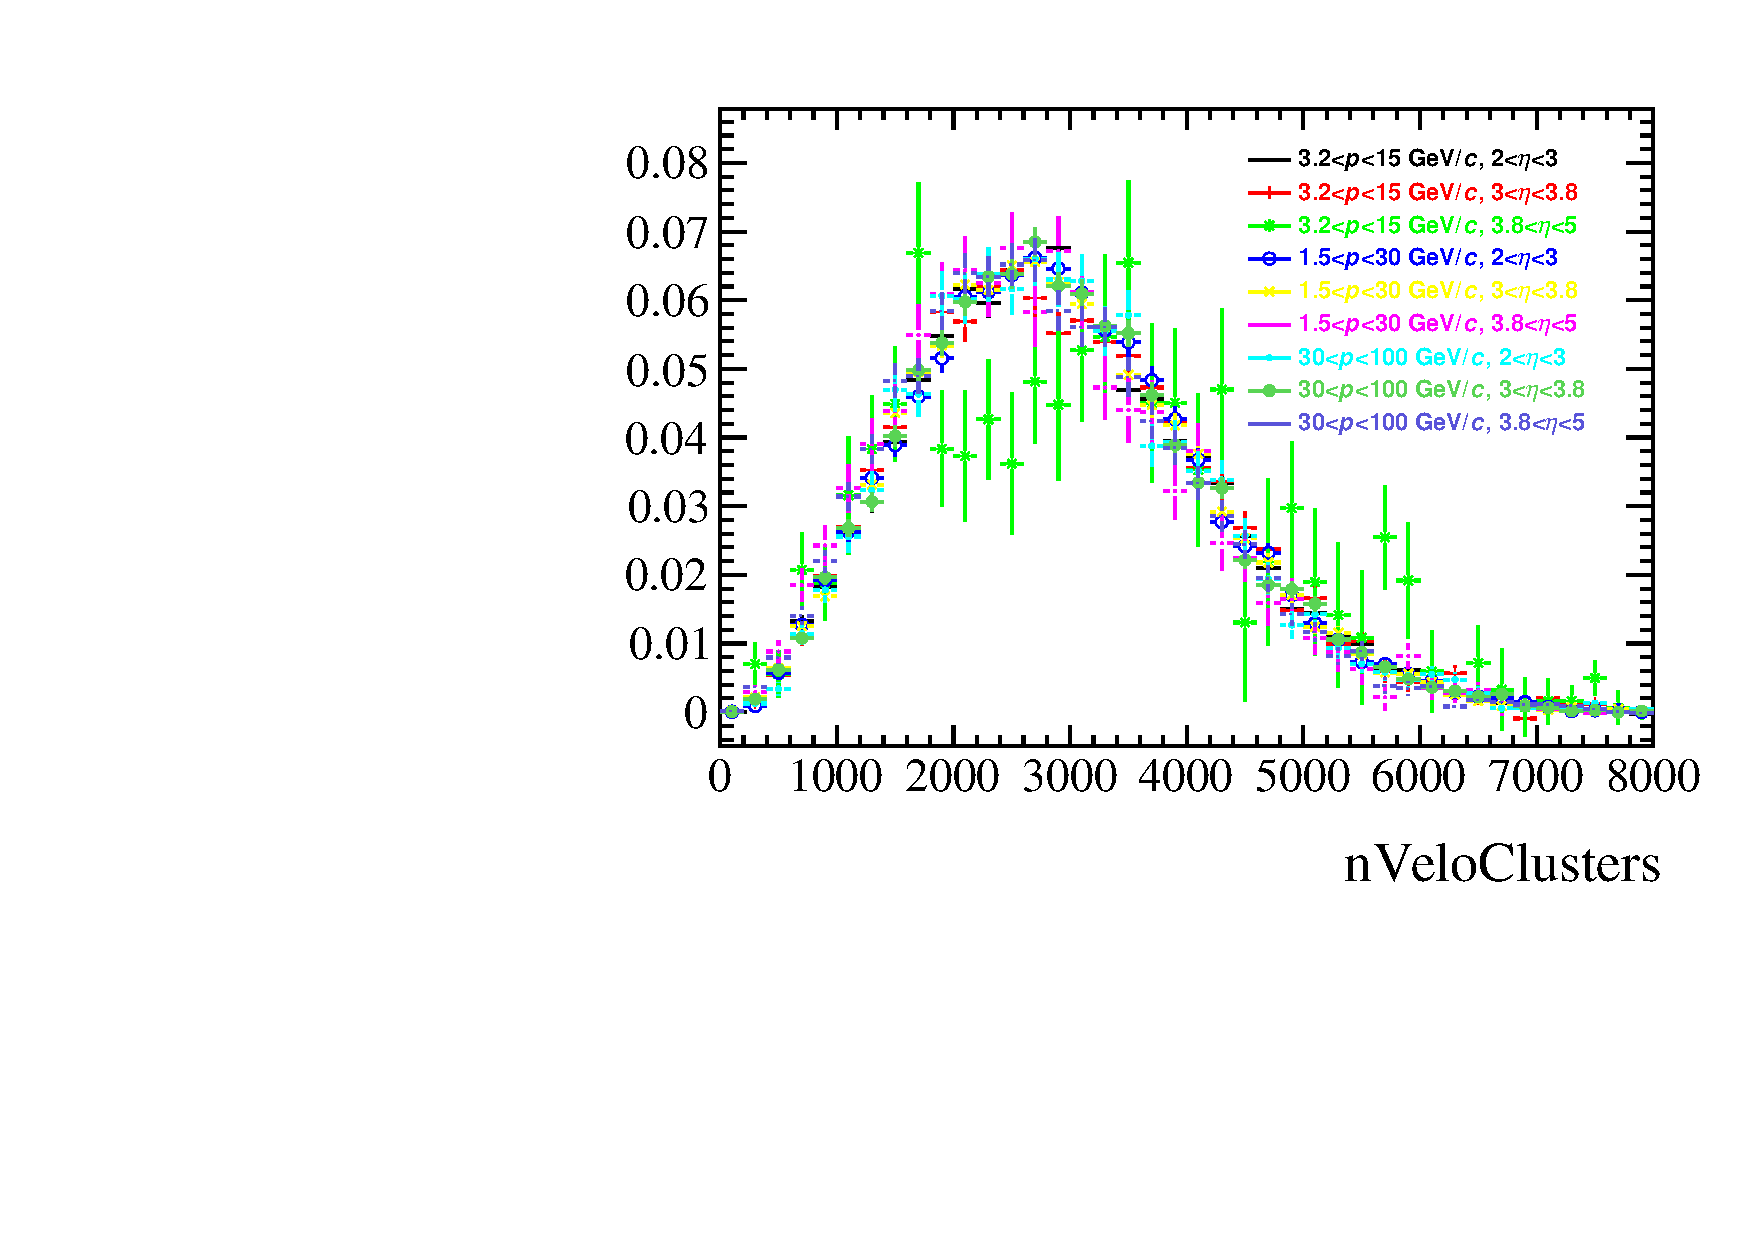
\includegraphics[width=0.45\linewidth]{PID/K_Passed_Ap}\put(-40,140){(d)}
    %\vspace*{-0.5cm}
    \caption{\small
    Normalised $\nVeloClusters$ distribution of \kaon PID calibration sample
    (top) before and (bottom) after PID selections in (left) forward and (right) backward rapidites
    in different kinematic regions.
    }
    \label{fig:PID_K}
\end{figure}
\begin{figure}[htbp]
    \centering
    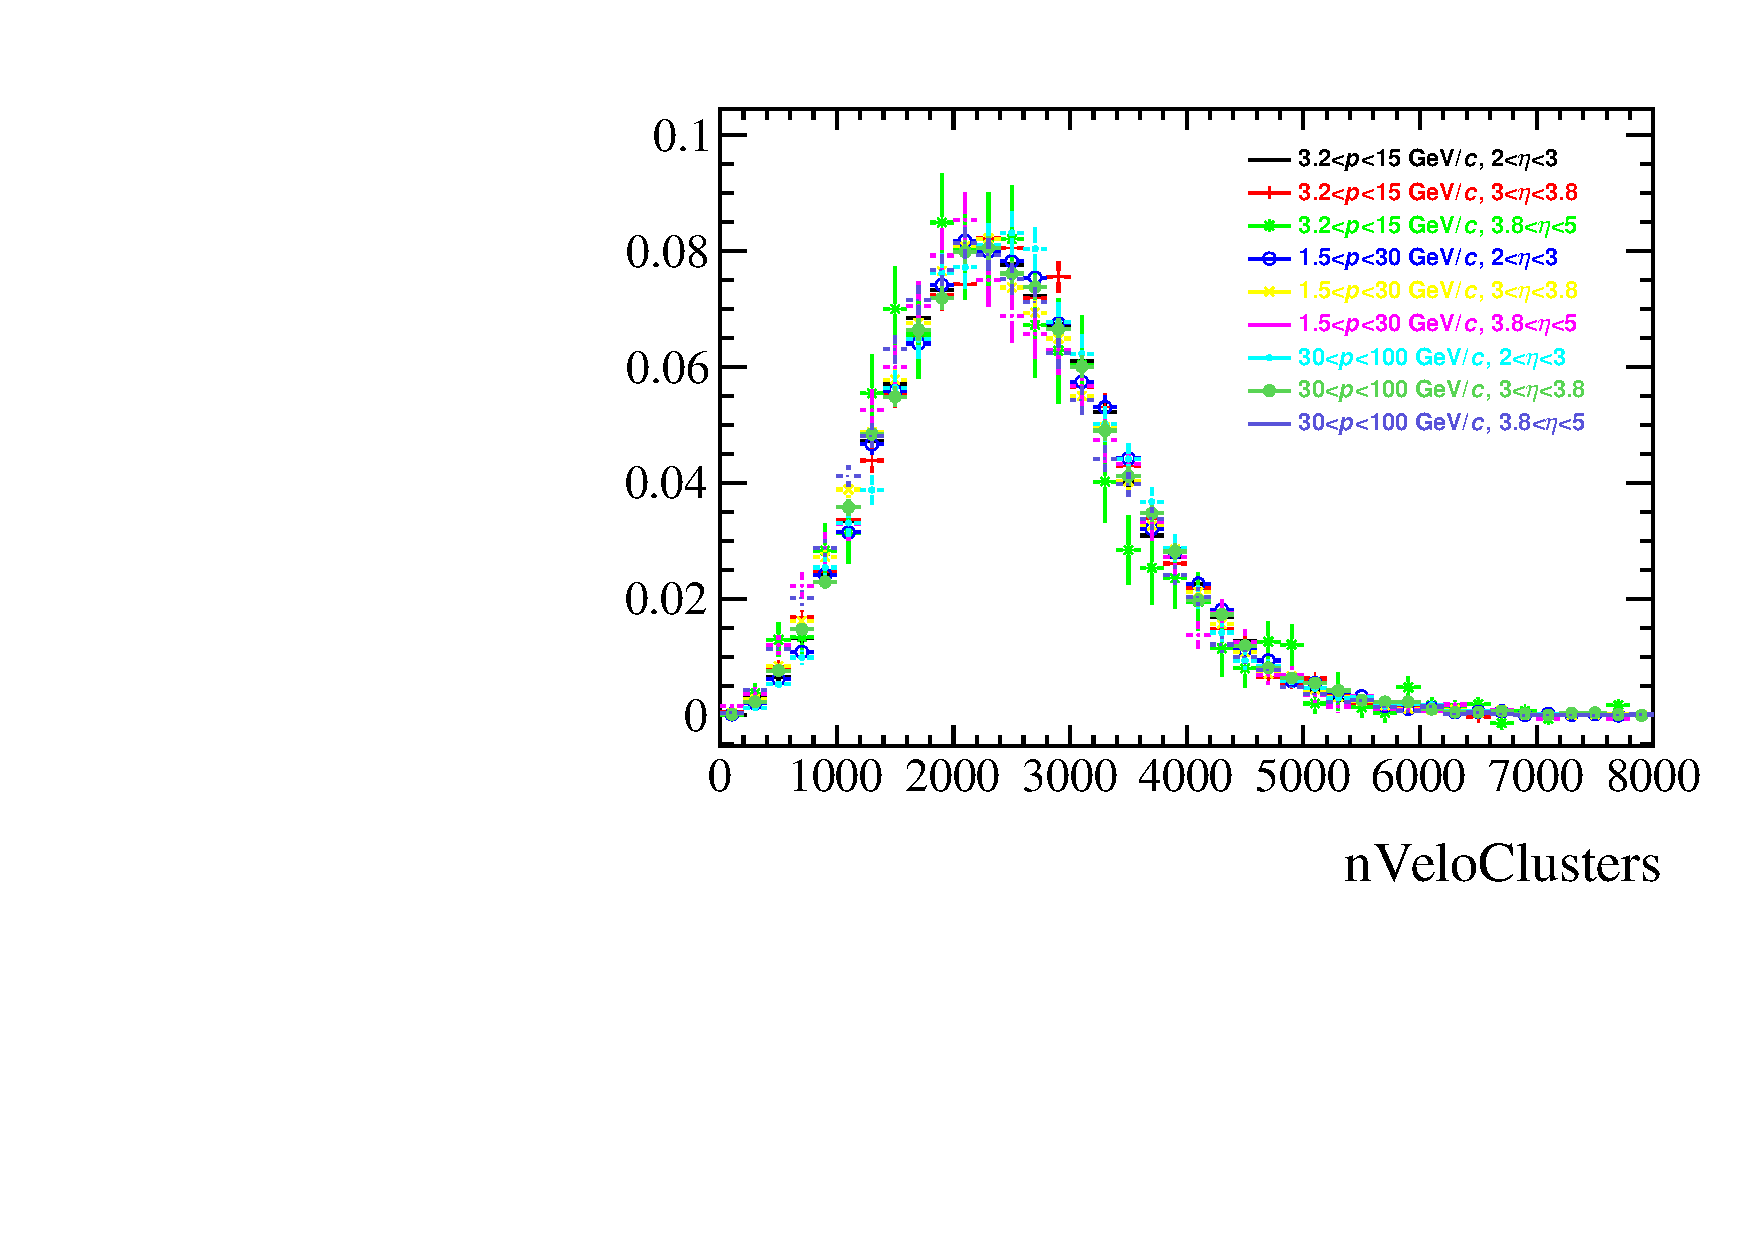
\includegraphics[width=0.45\linewidth]{PID/Pi_Total_pA}\put(-40,140){(a)}
    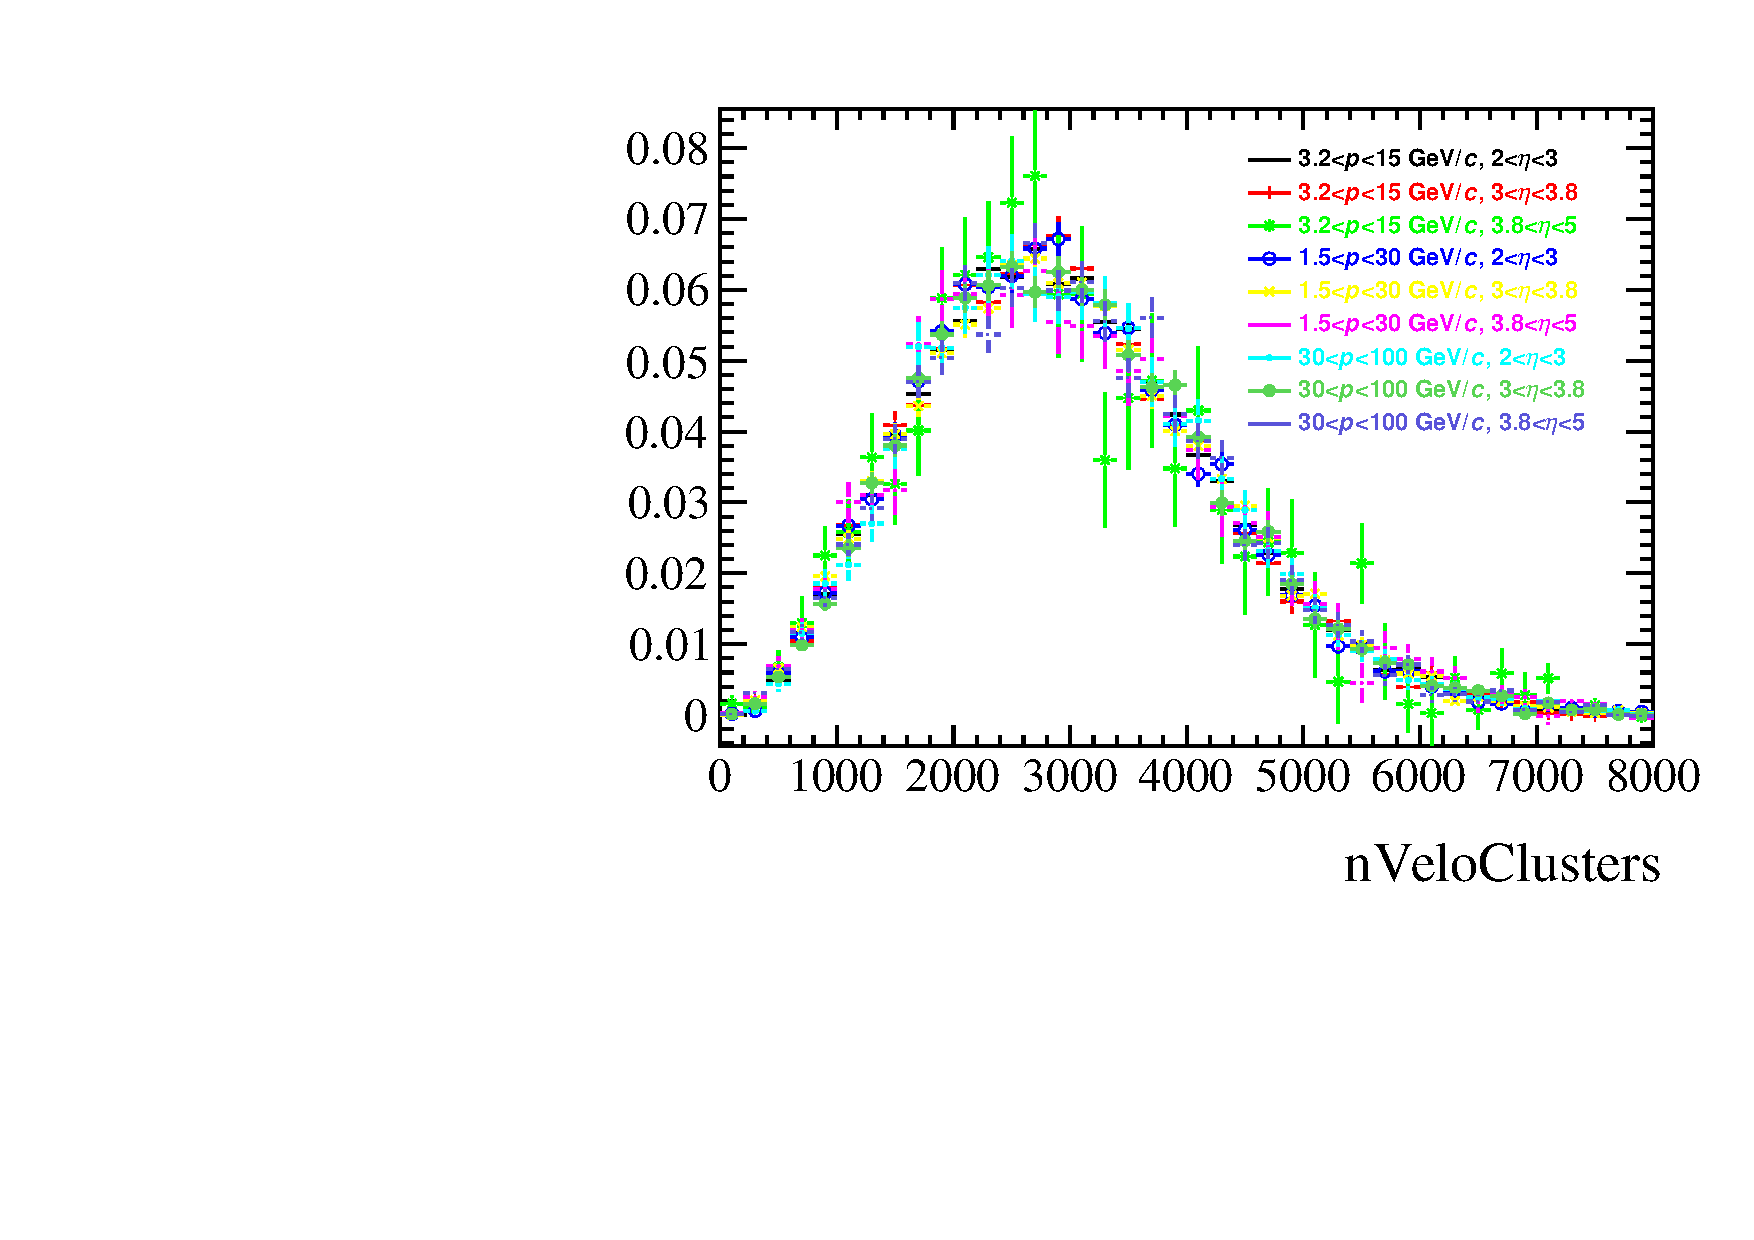
\includegraphics[width=0.45\linewidth]{PID/Pi_Total_Ap}\put(-40,140){(b)}

    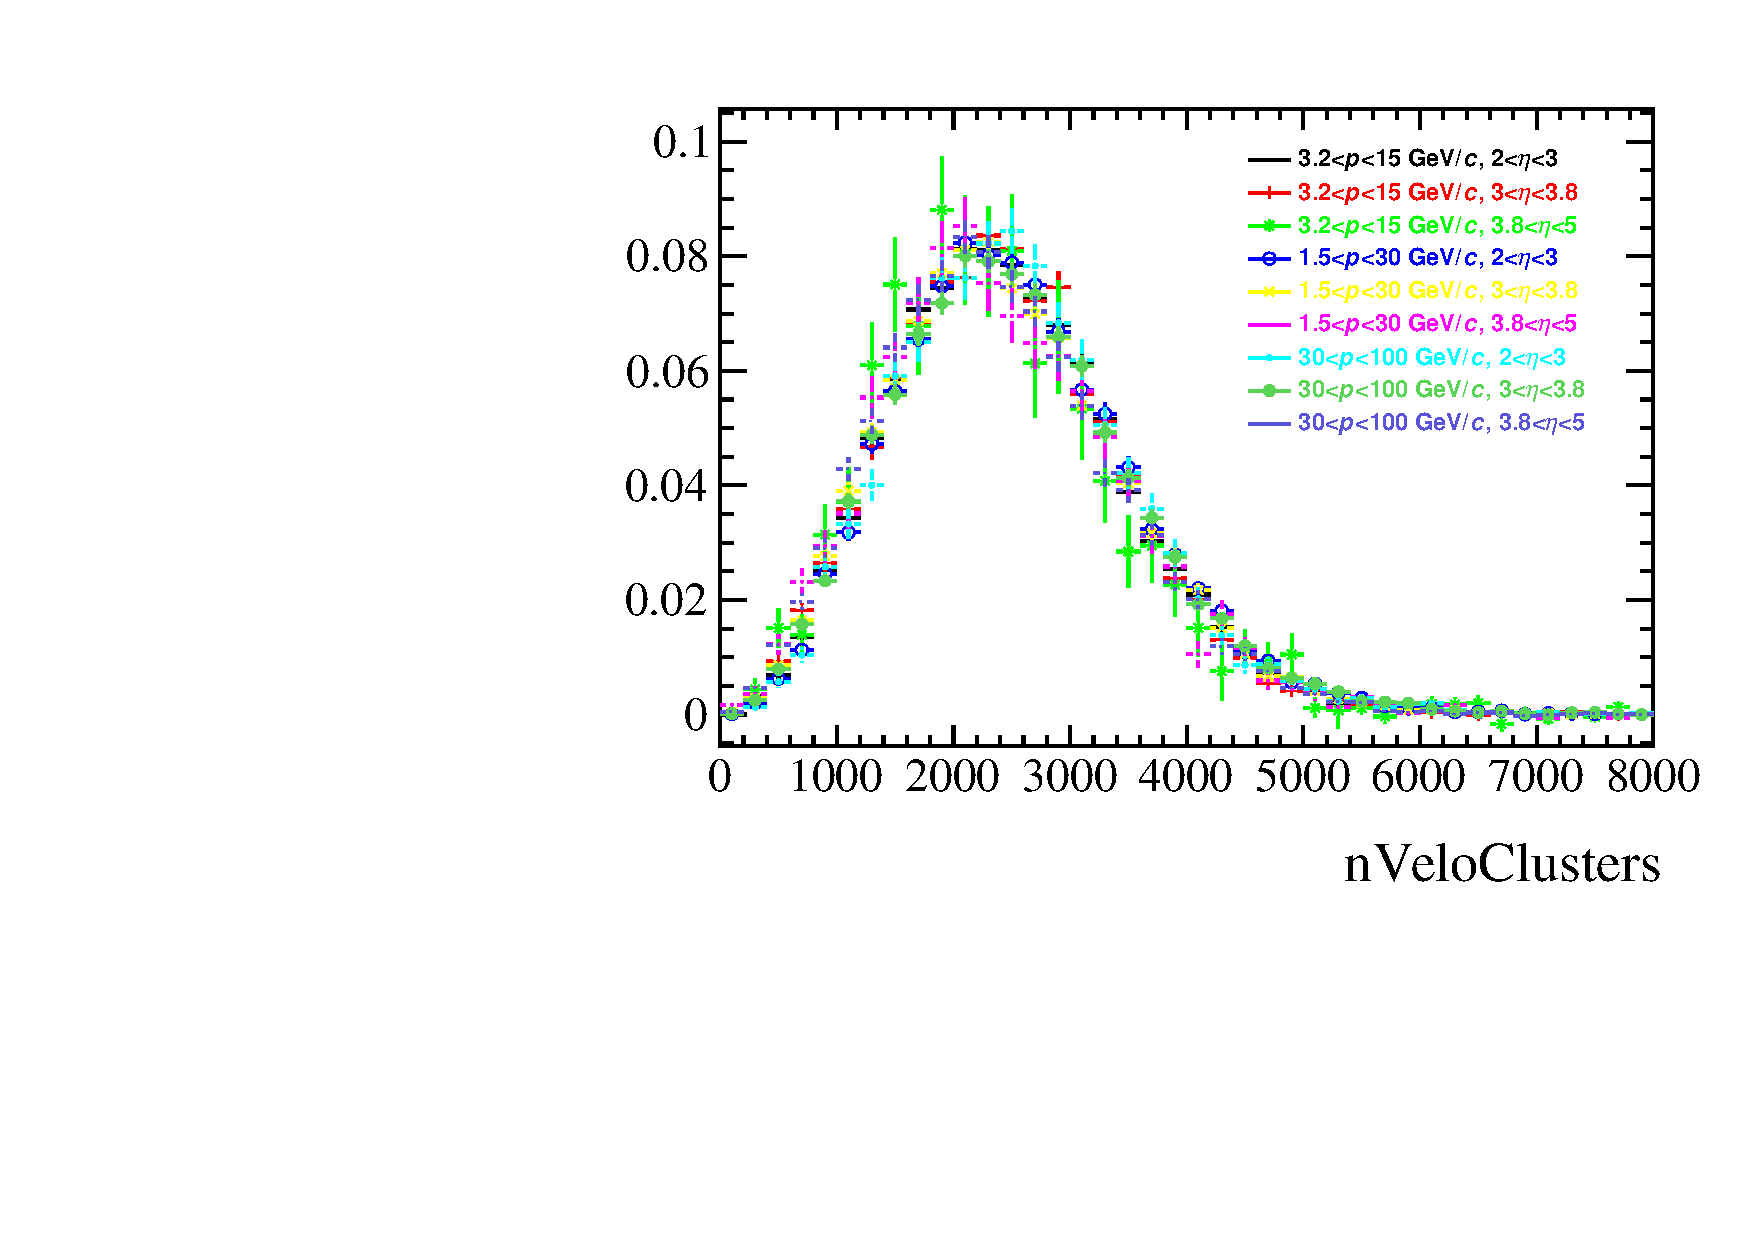
\includegraphics[width=0.45\linewidth]{PID/Pi_Passed_pA}\put(-40,140){(c)}
    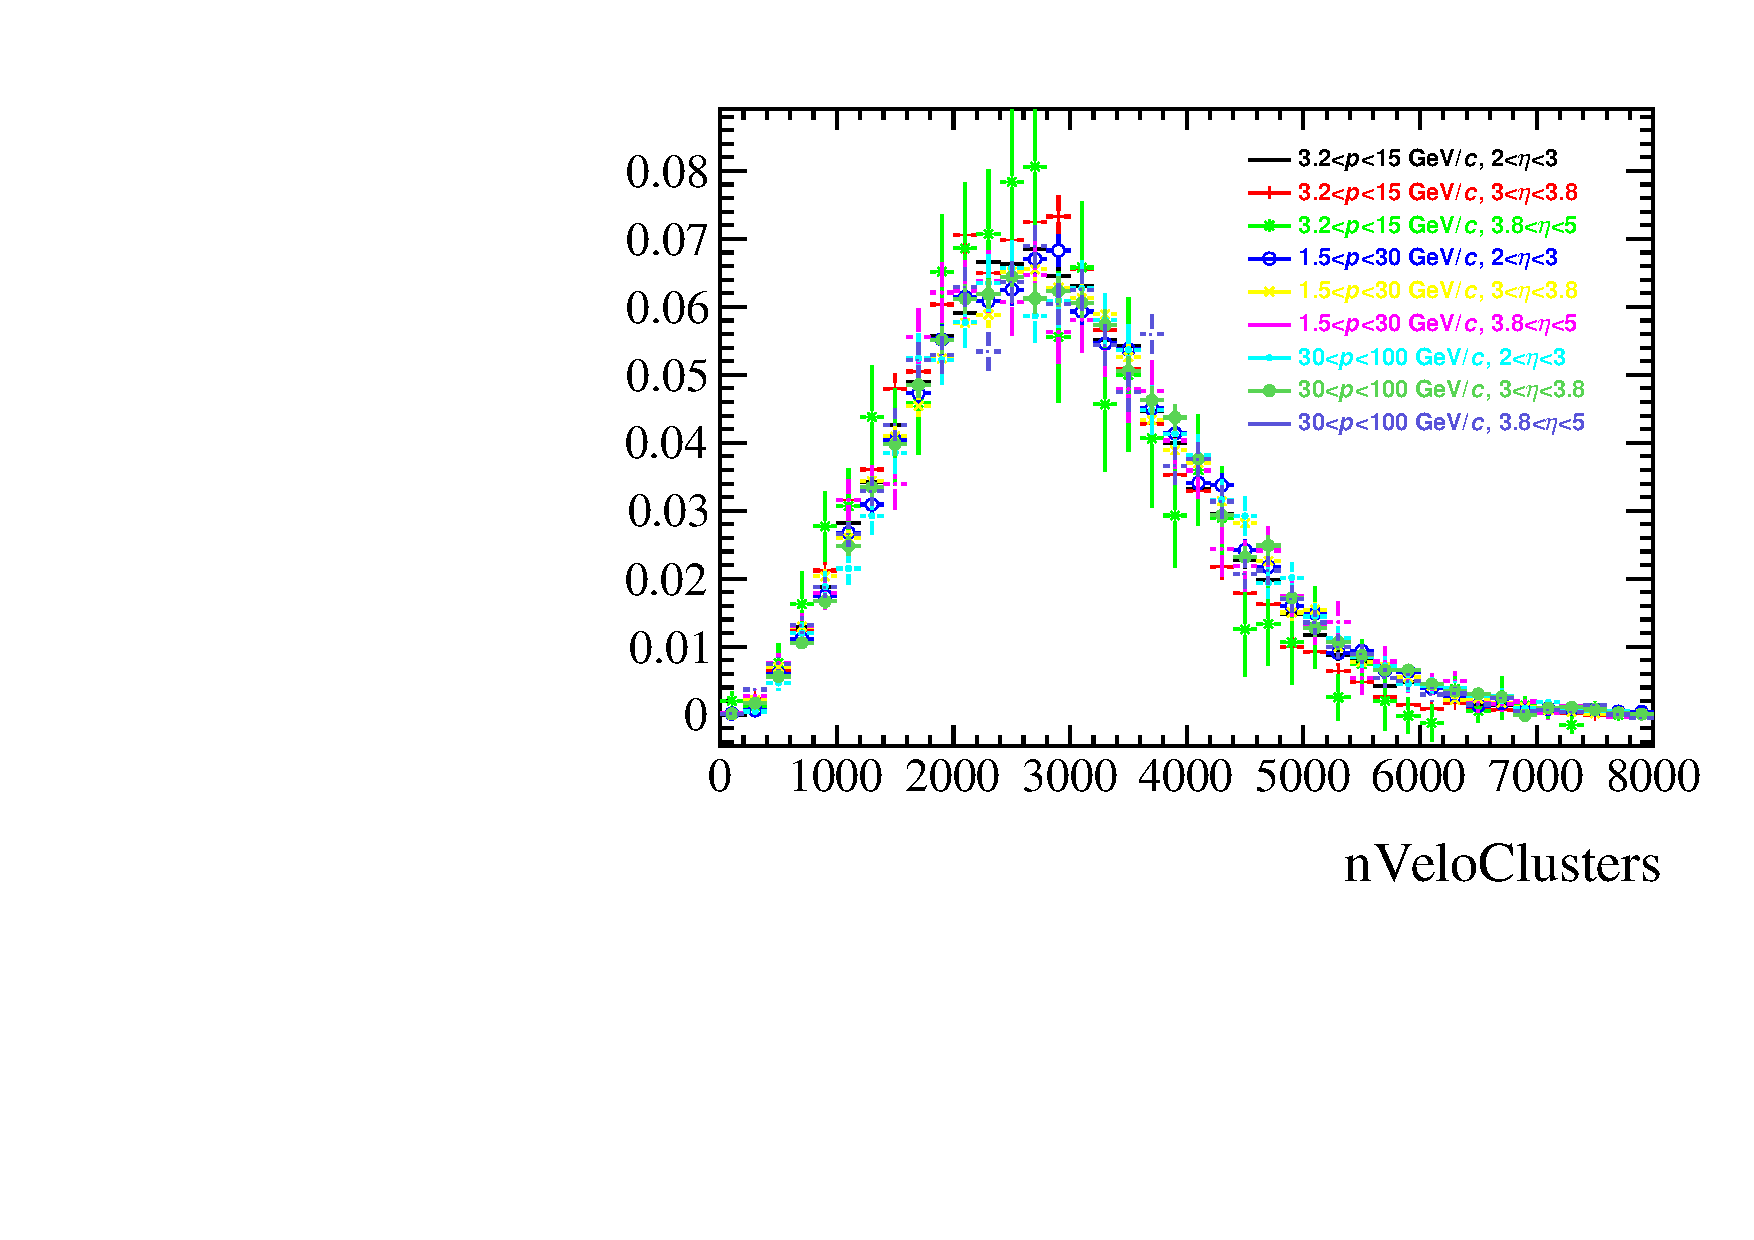
\includegraphics[width=0.45\linewidth]{PID/Pi_Passed_Ap}\put(-40,140){(d)}
    %\vspace*{-0.5cm}
    \caption{\small
    Normalised $\nVeloClusters$ distribution of \pion PID calibration sample
    (top) before and (bottom) after PID selections in (left) forward and (right) backward rapidites
    in different kinematic regions.
    }
    \label{fig:PID_pi}
\end{figure}
\begin{figure}[htbp]
    \centering
    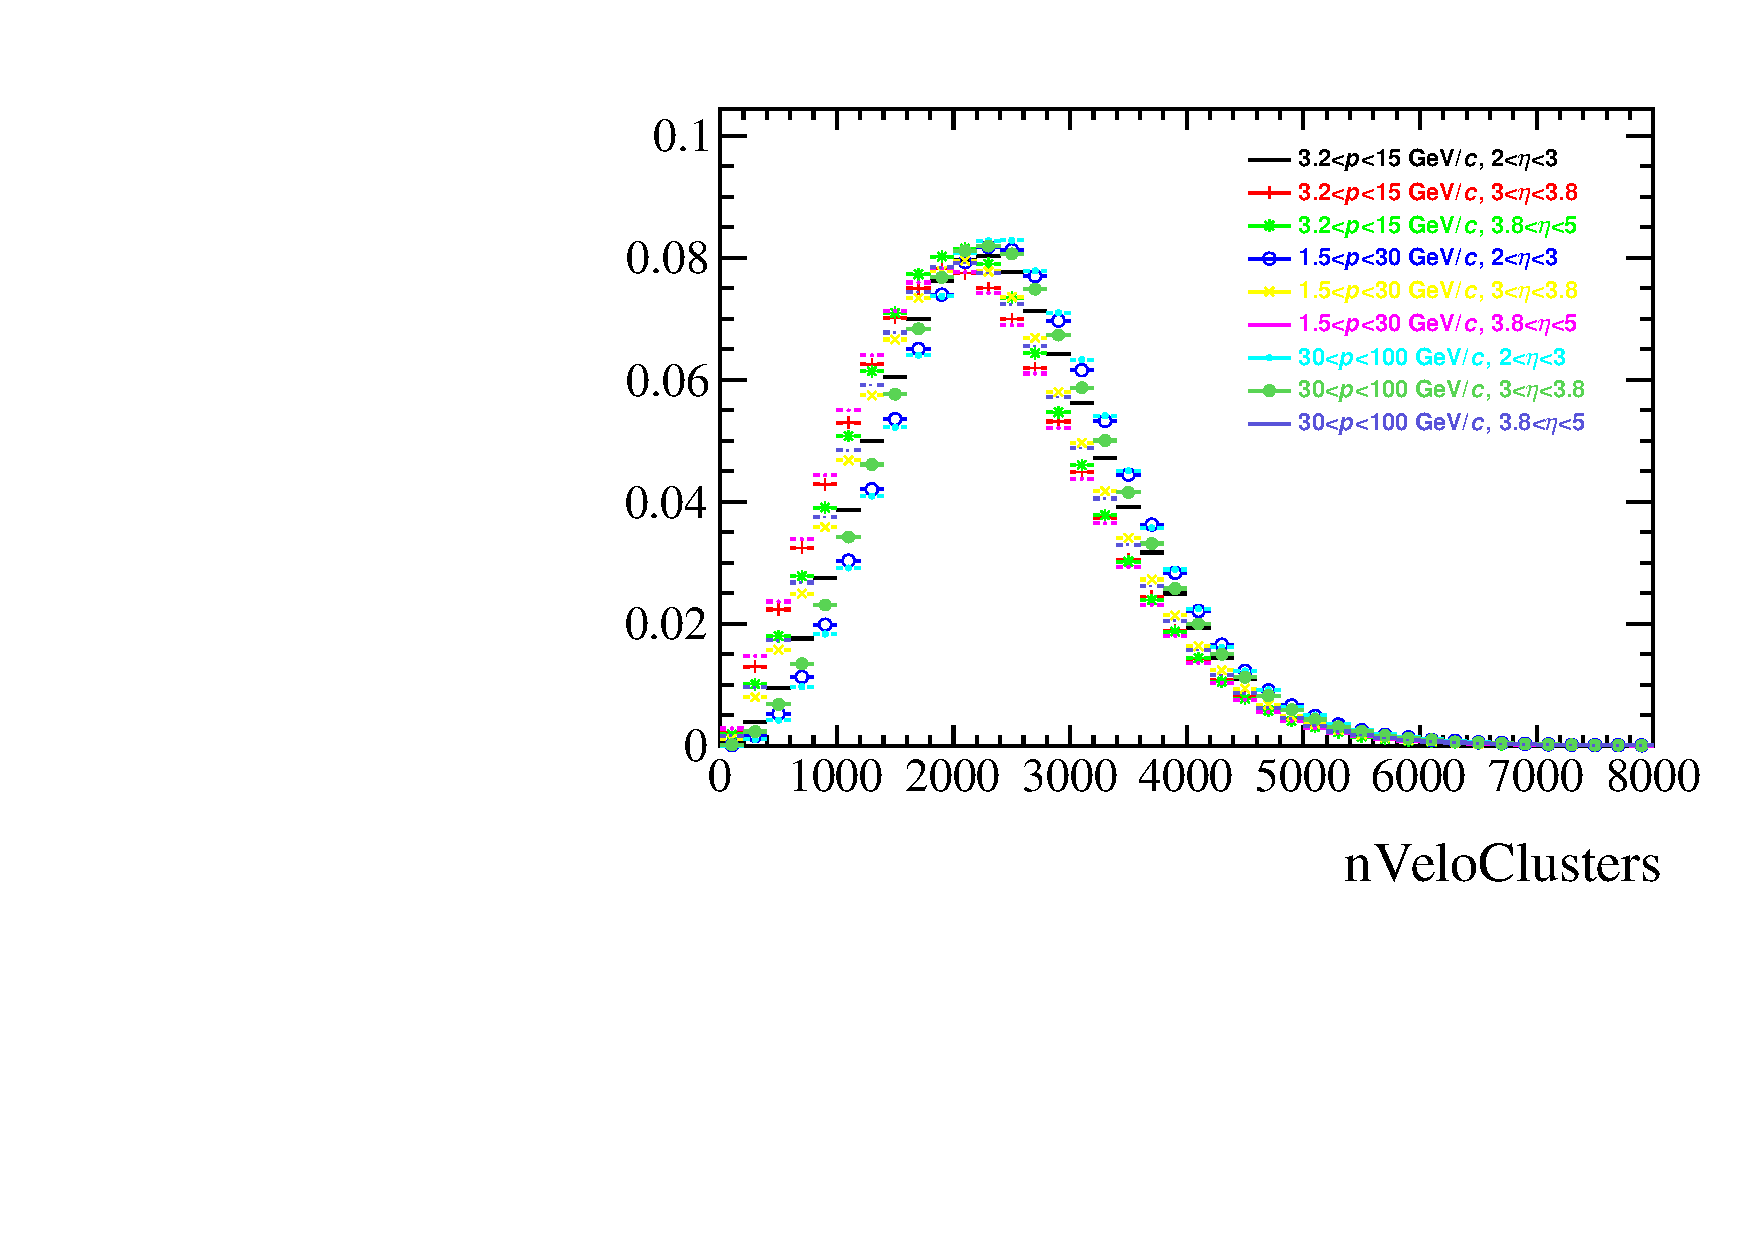
\includegraphics[width=0.45\linewidth]{PID/P_Total_pA}\put(-40,140){(a)}
    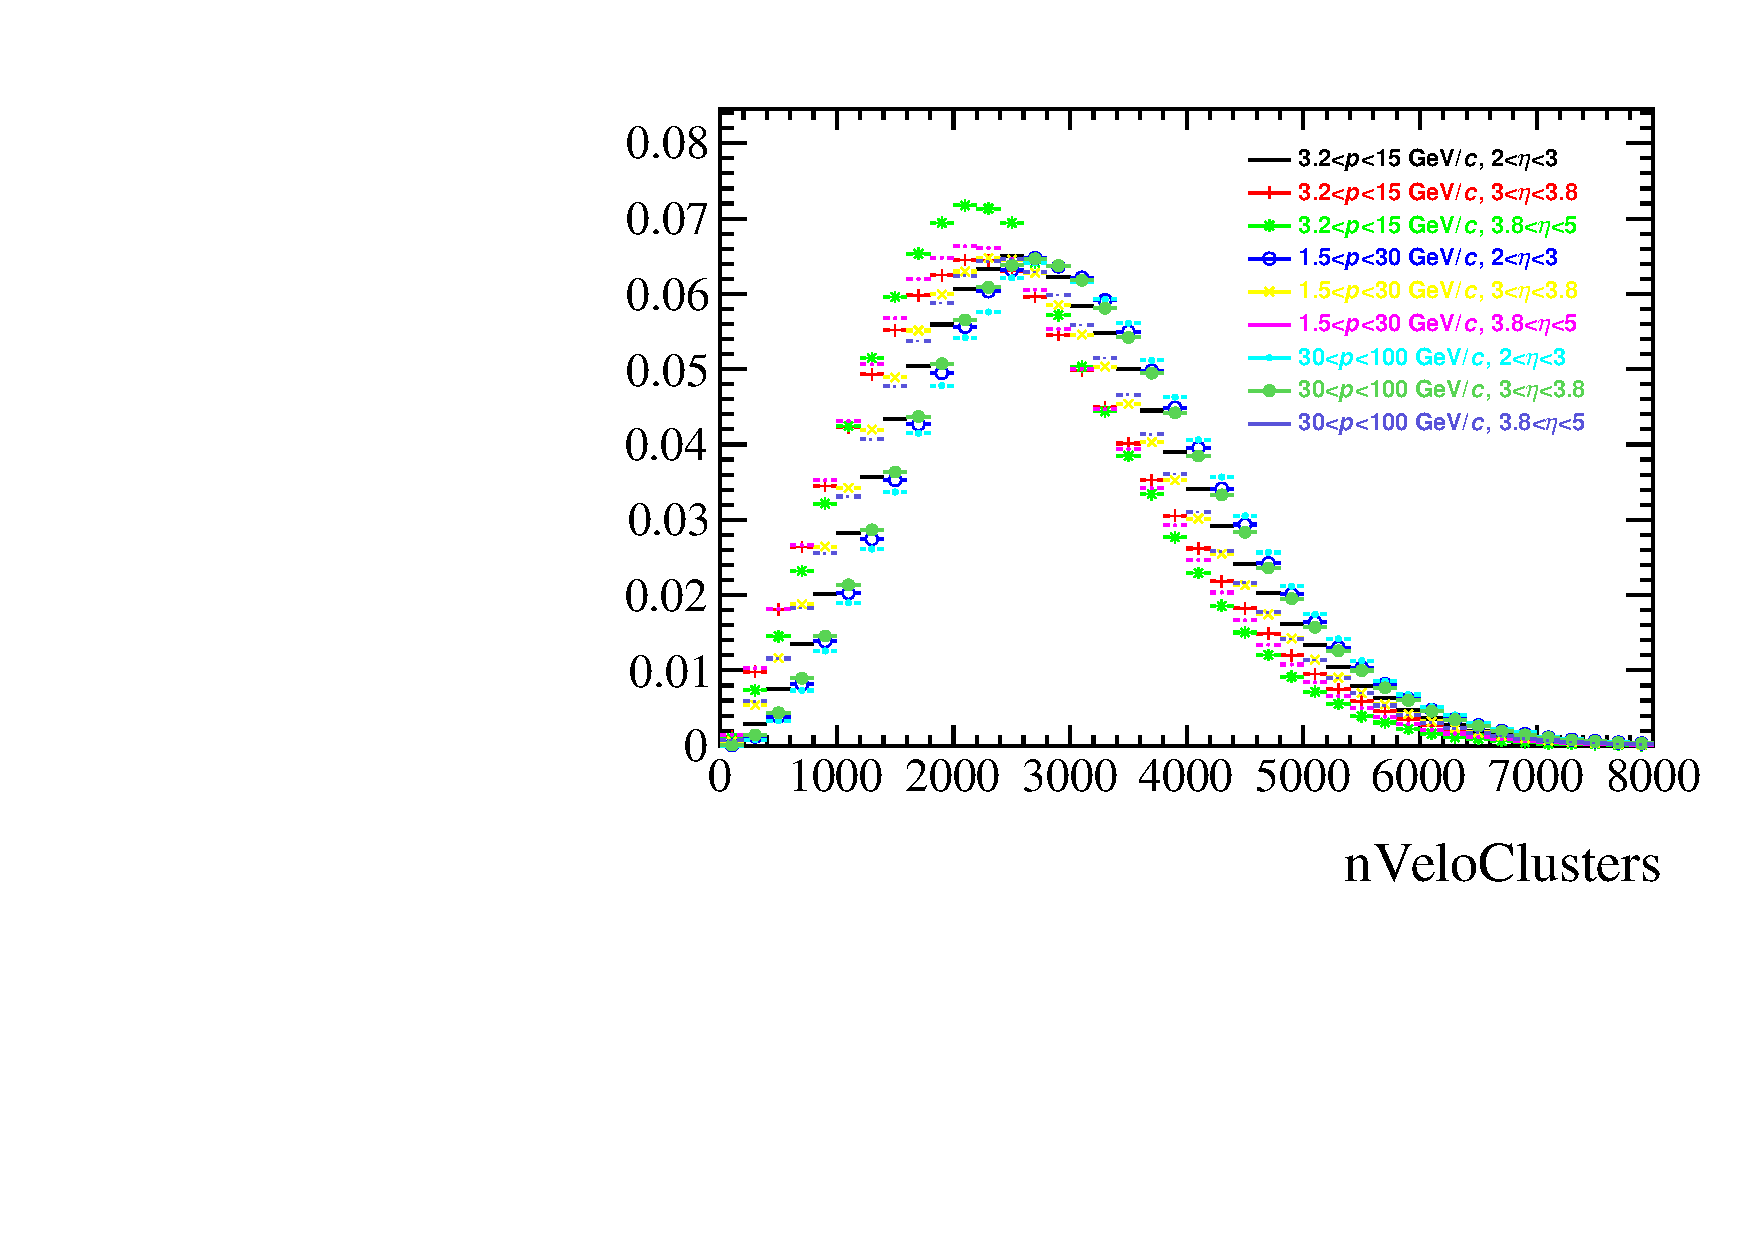
\includegraphics[width=0.45\linewidth]{PID/P_Total_Ap}\put(-40,140){(b)}

    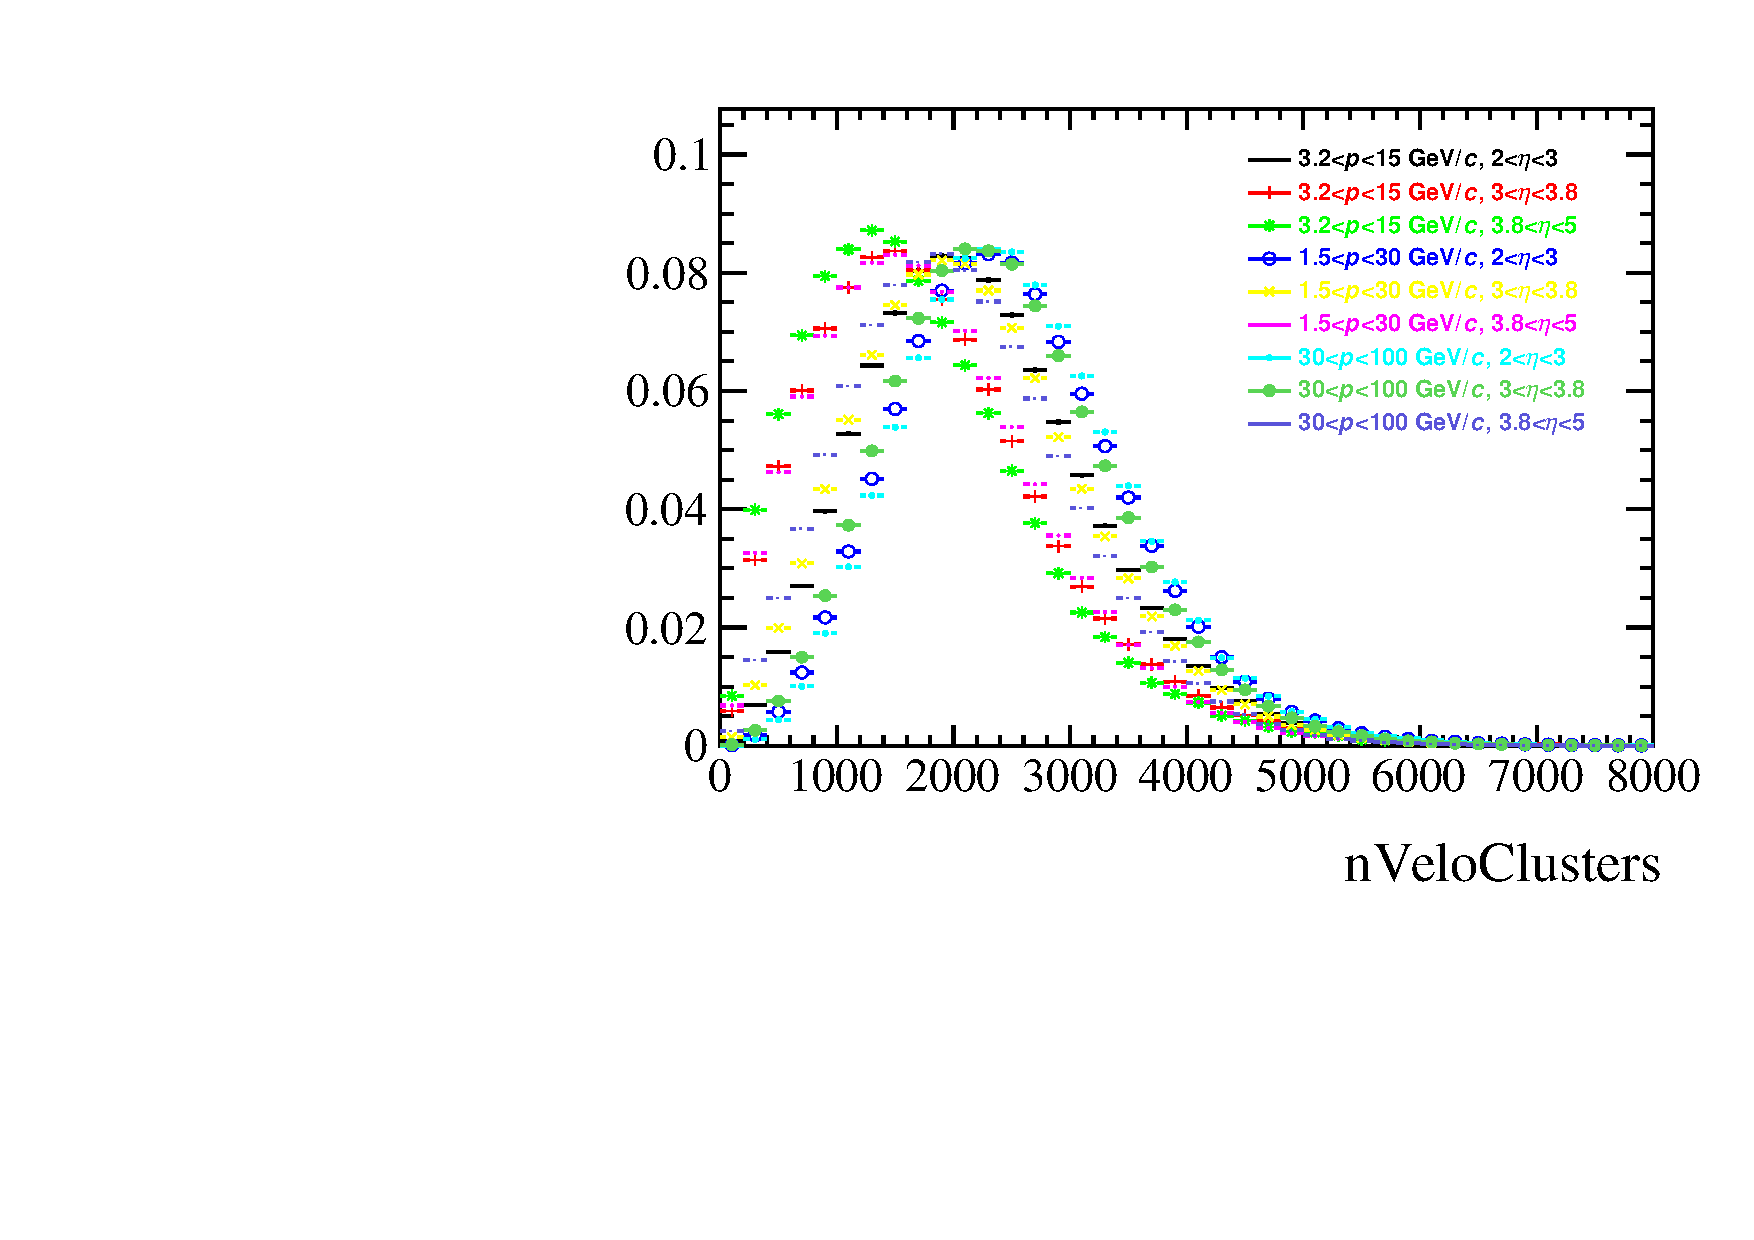
\includegraphics[width=0.45\linewidth]{PID/P_Passed_pA}\put(-40,140){(c)}
    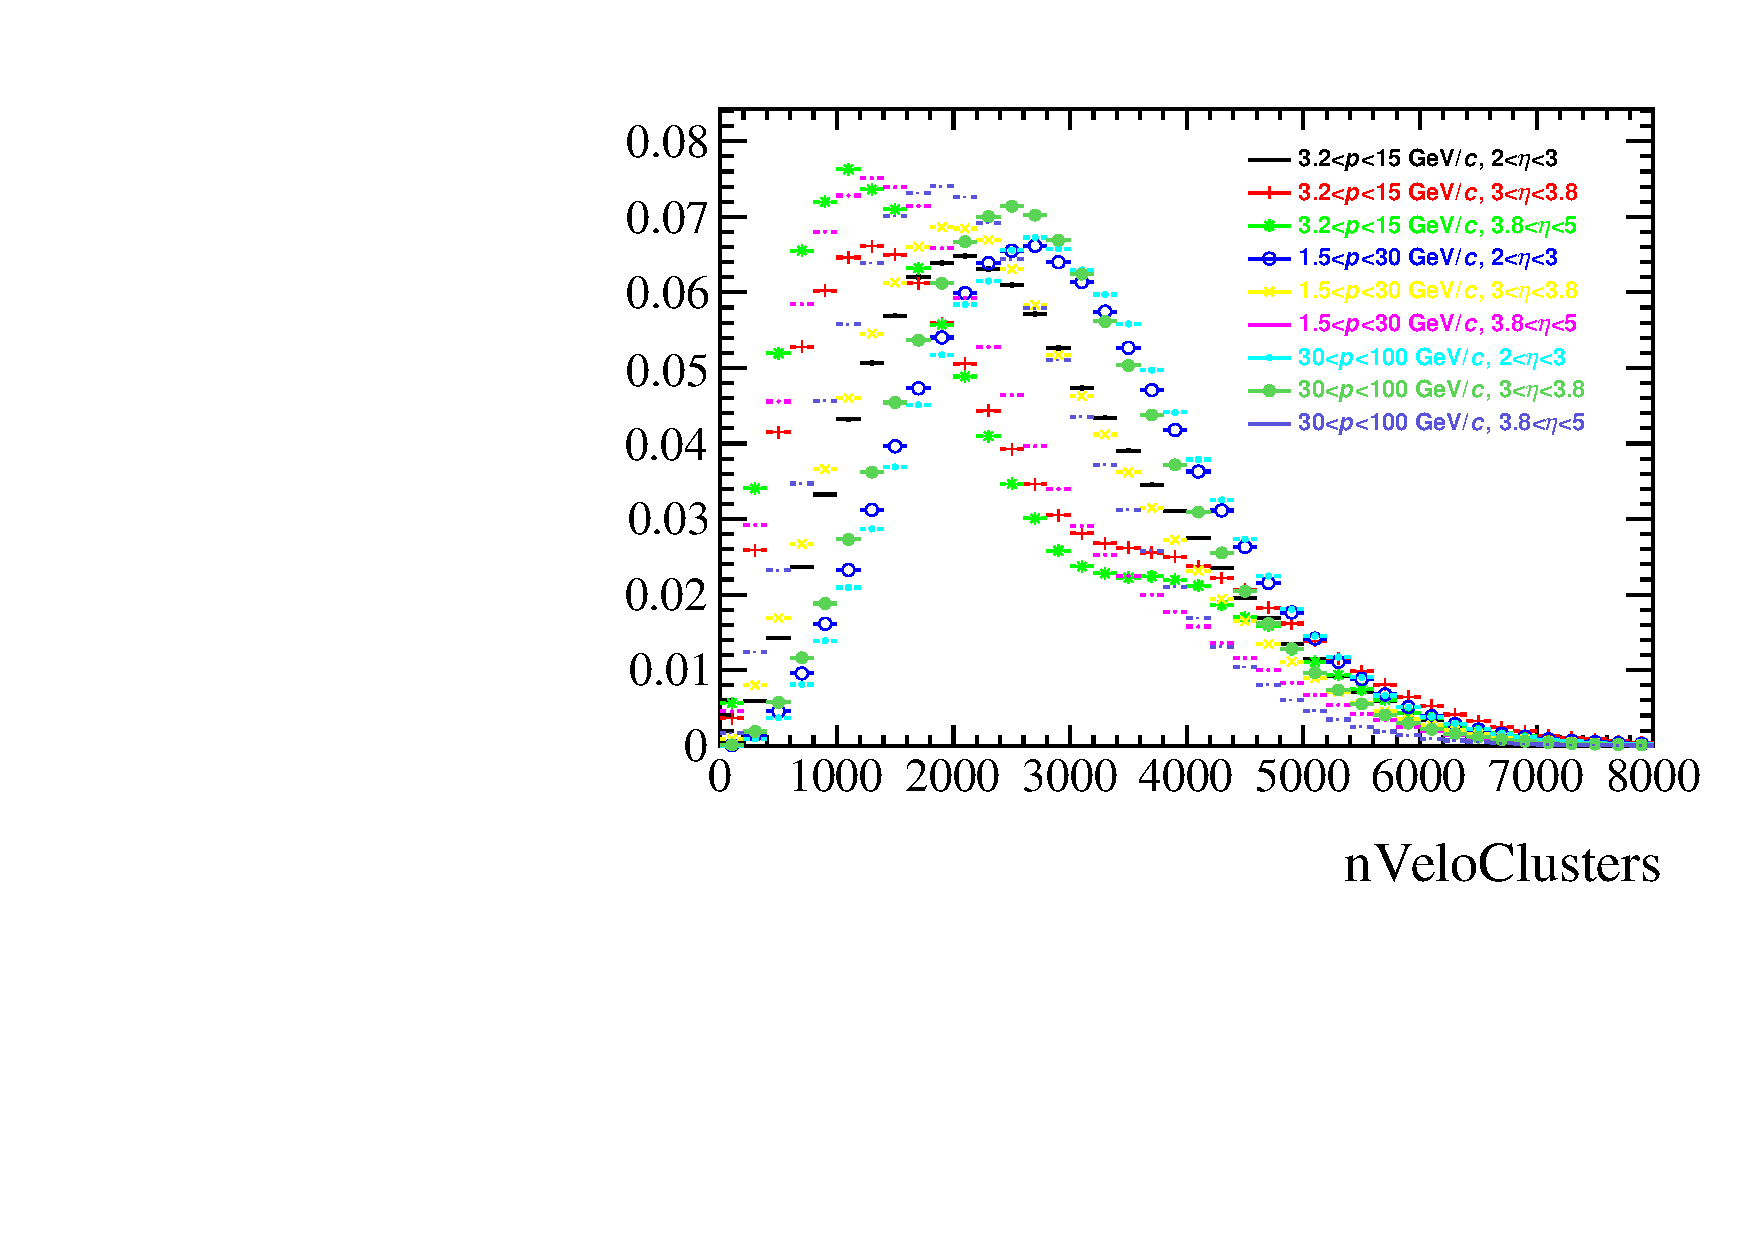
\includegraphics[width=0.45\linewidth]{PID/P_Passed_Ap}\put(-40,140){(d)}
    %\vspace*{-0.5cm}
    \caption{\small
    Normalised $\nVeloClusters$ distribution of \proton PID calibration sample
    (top) before and (bottom) after PID selections in (left) forward and (right) backward rapidites
    in different kinematic regions.
    }
    \label{fig:PID_p}
\end{figure}

The $\varepsilon_\mathrm{PID}(p,\eta)$ and $\varepsilon_\mathrm{PID}$ for \kaon and \pion are shown
in Fig.~\ref{fig:PID2DK} and Fig.~\ref{fig:PID2Dpi} respectively.
\begin{figure}[htbp]
    \centering
    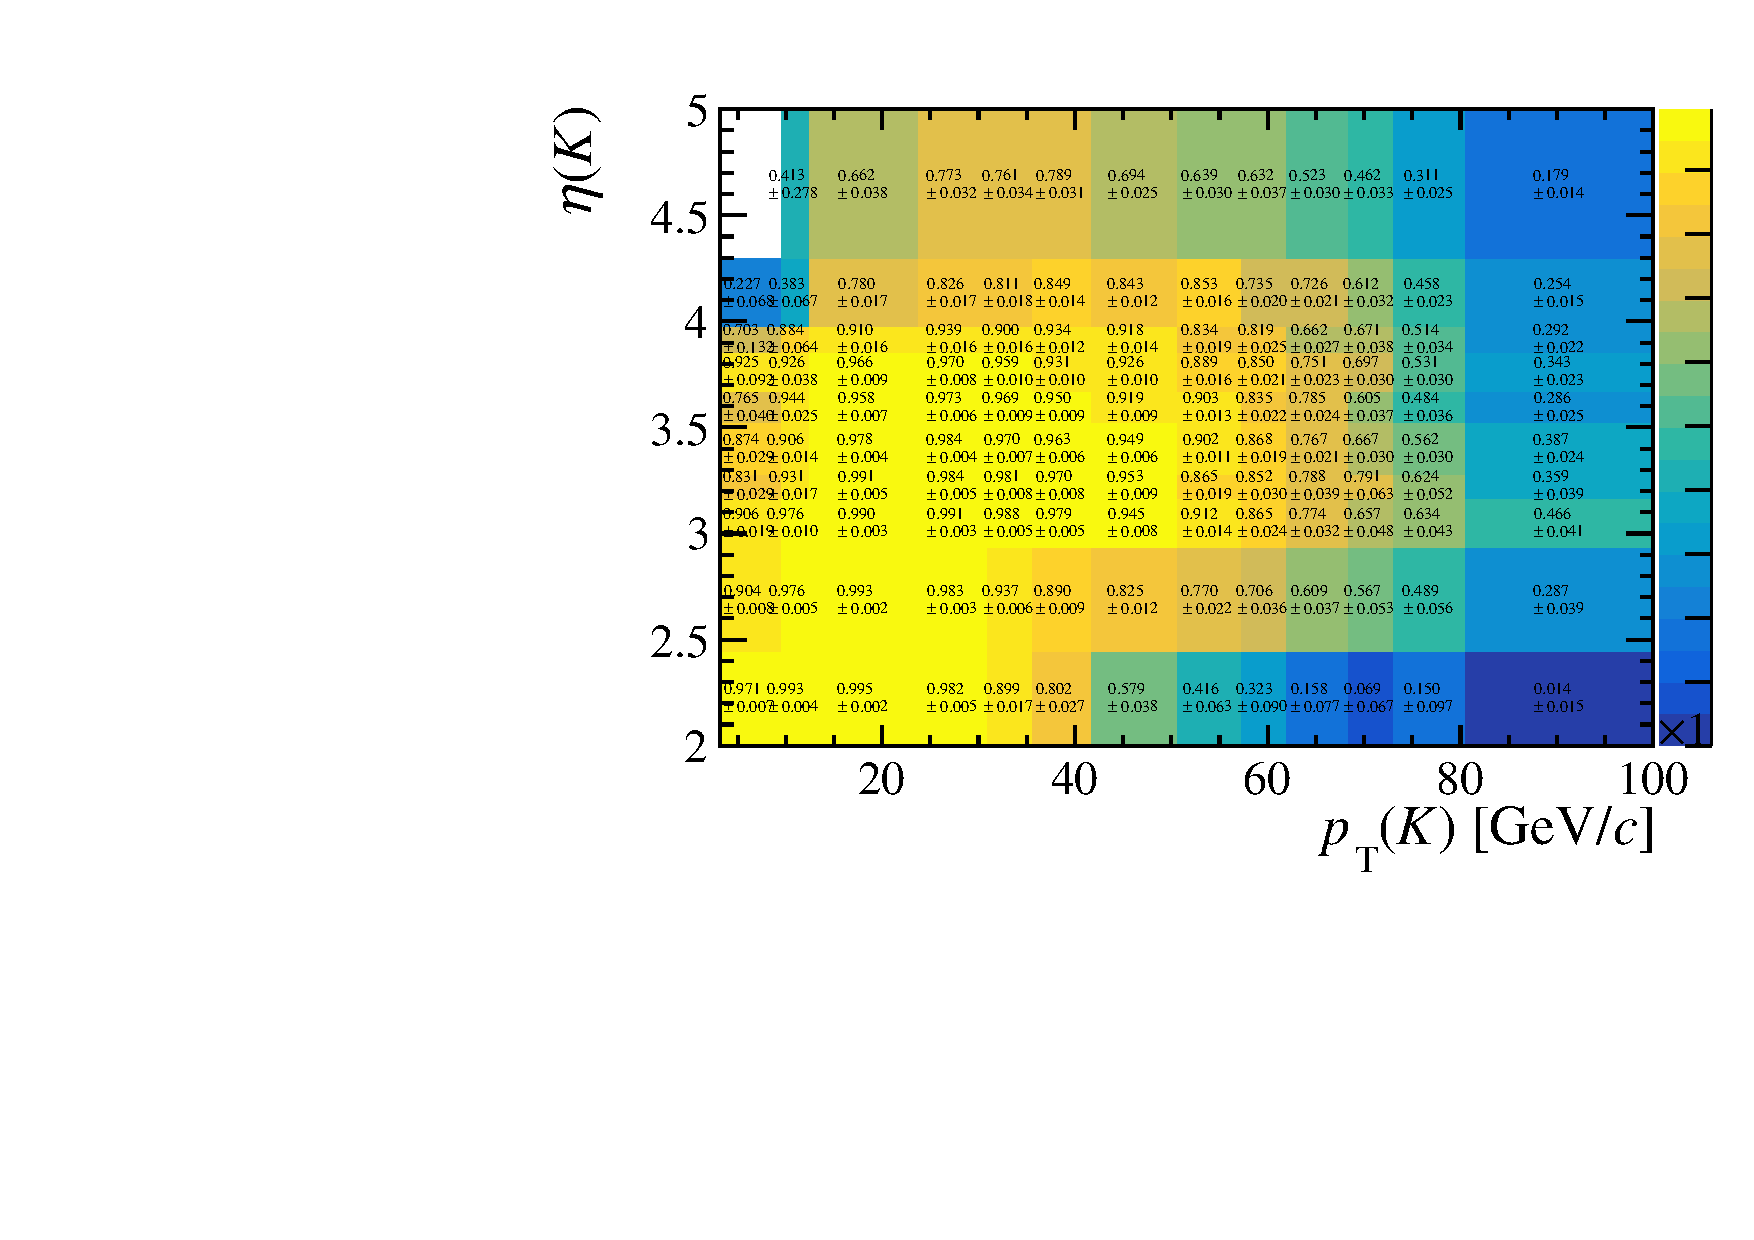
\includegraphics[width=0.45\linewidth]{PID/K_PID_p_eta_pA}\put(-40,140){(a)}
    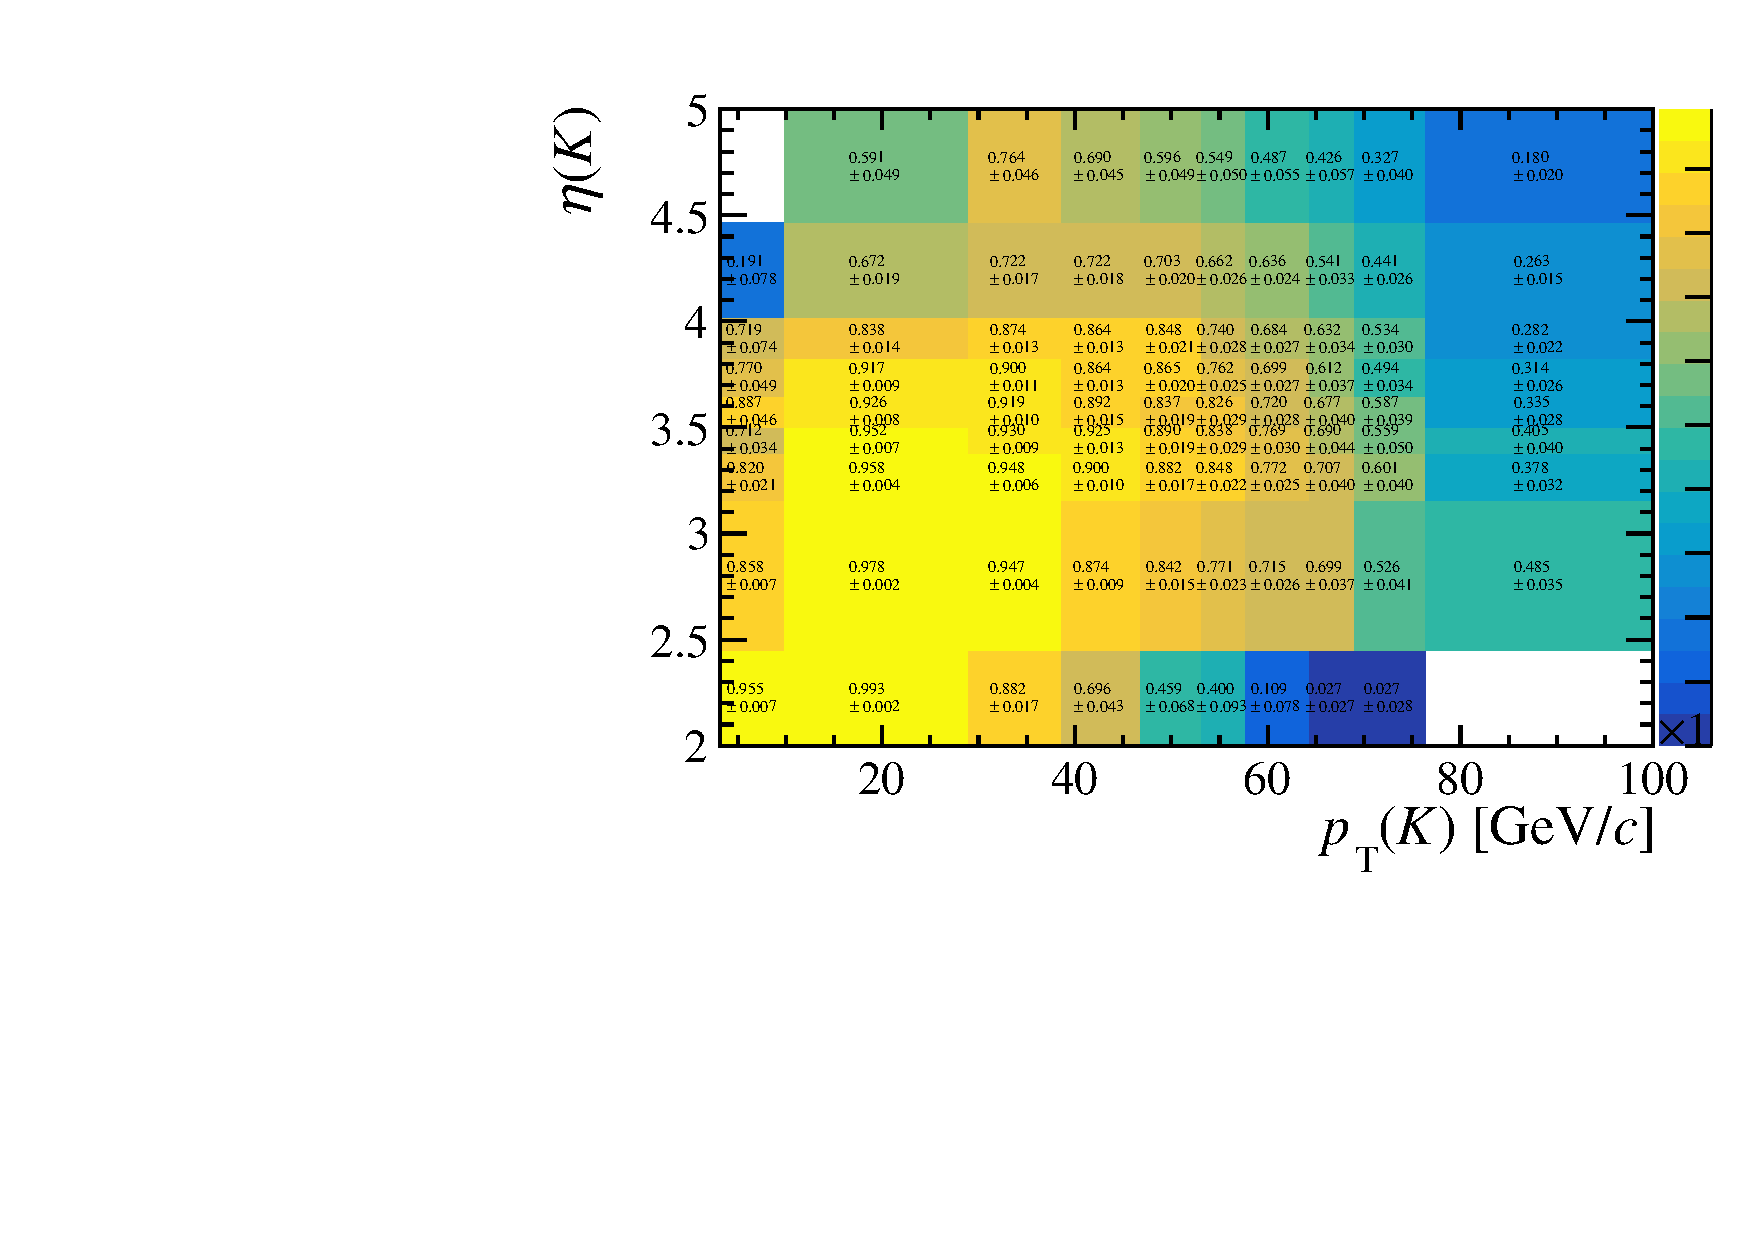
\includegraphics[width=0.45\linewidth]{PID/K_PID_p_eta_Ap}\put(-40,140){(b)}

    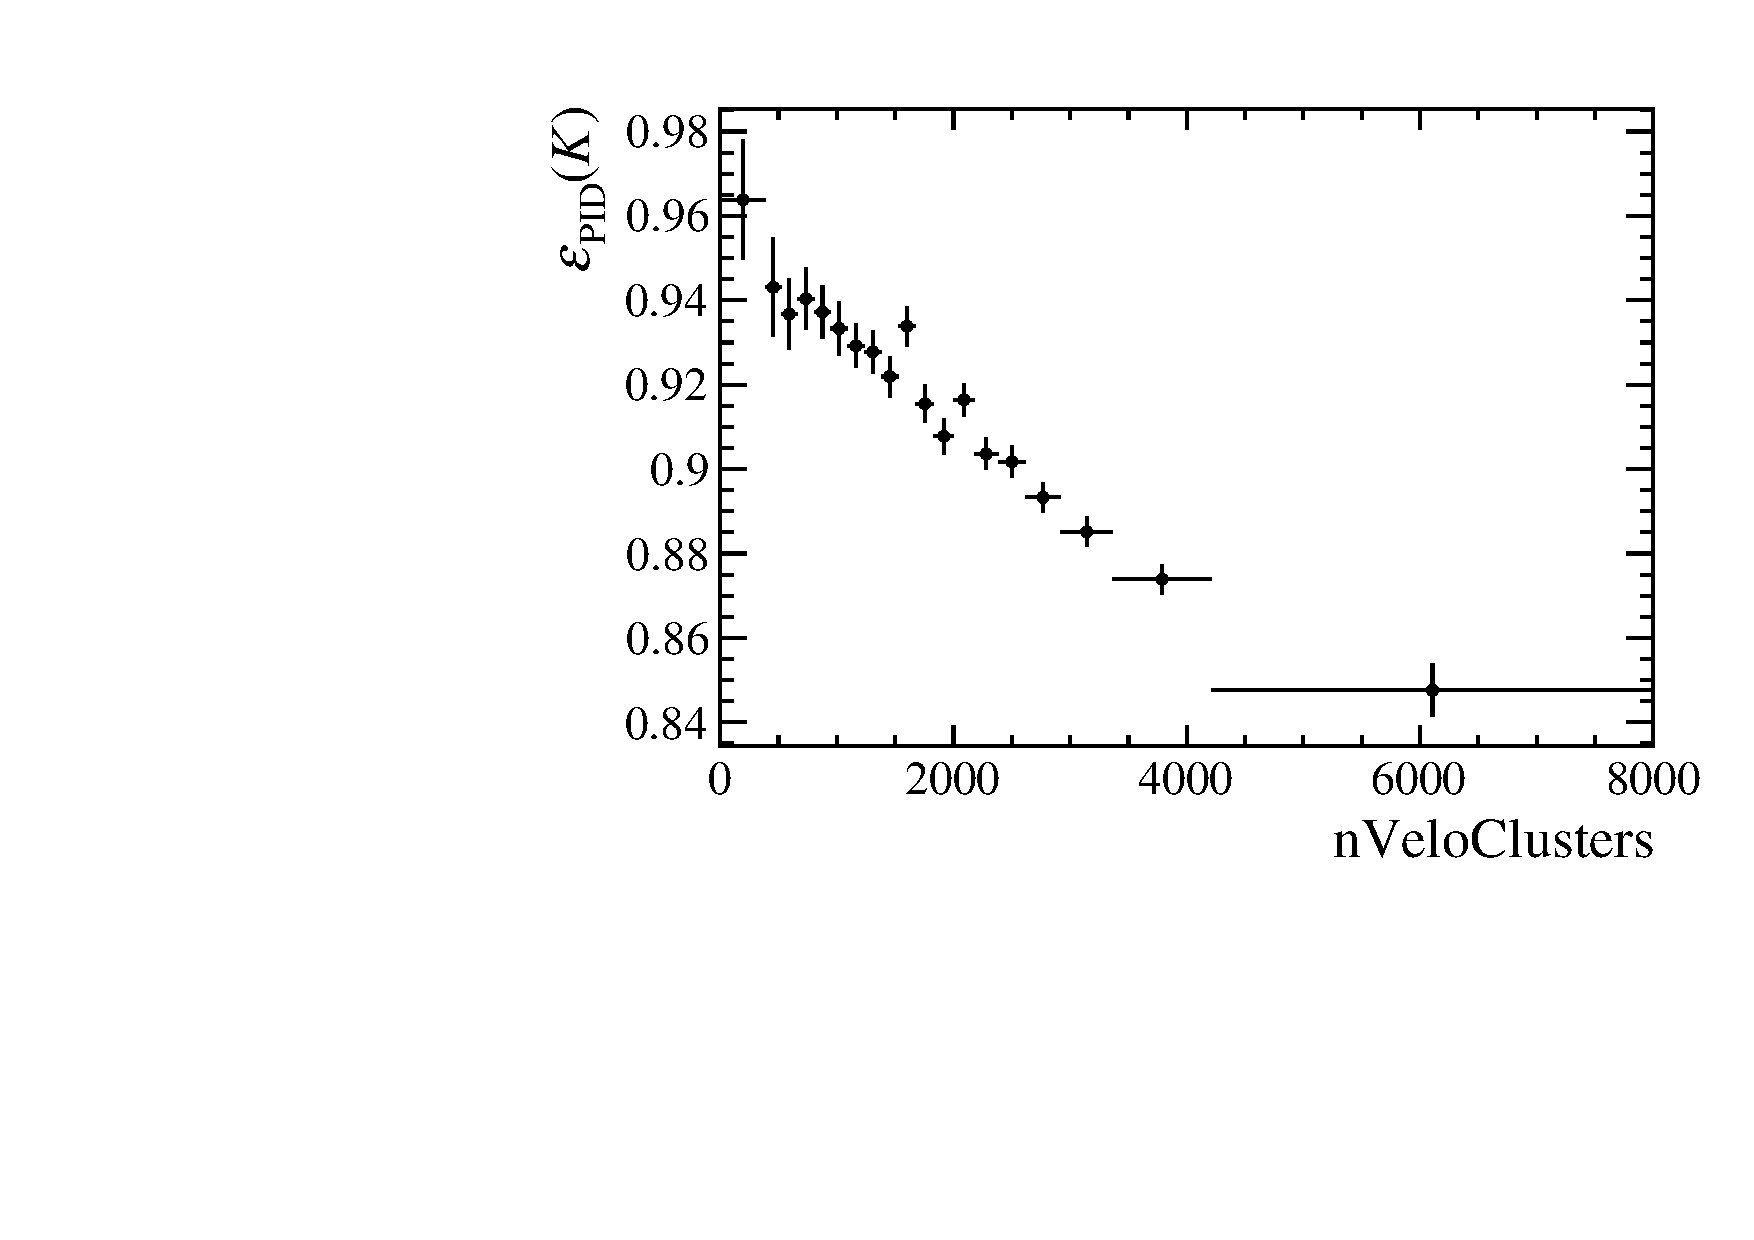
\includegraphics[width=0.45\linewidth]{PID/K_PID_nv_pA}\put(-40,140){(c)}
    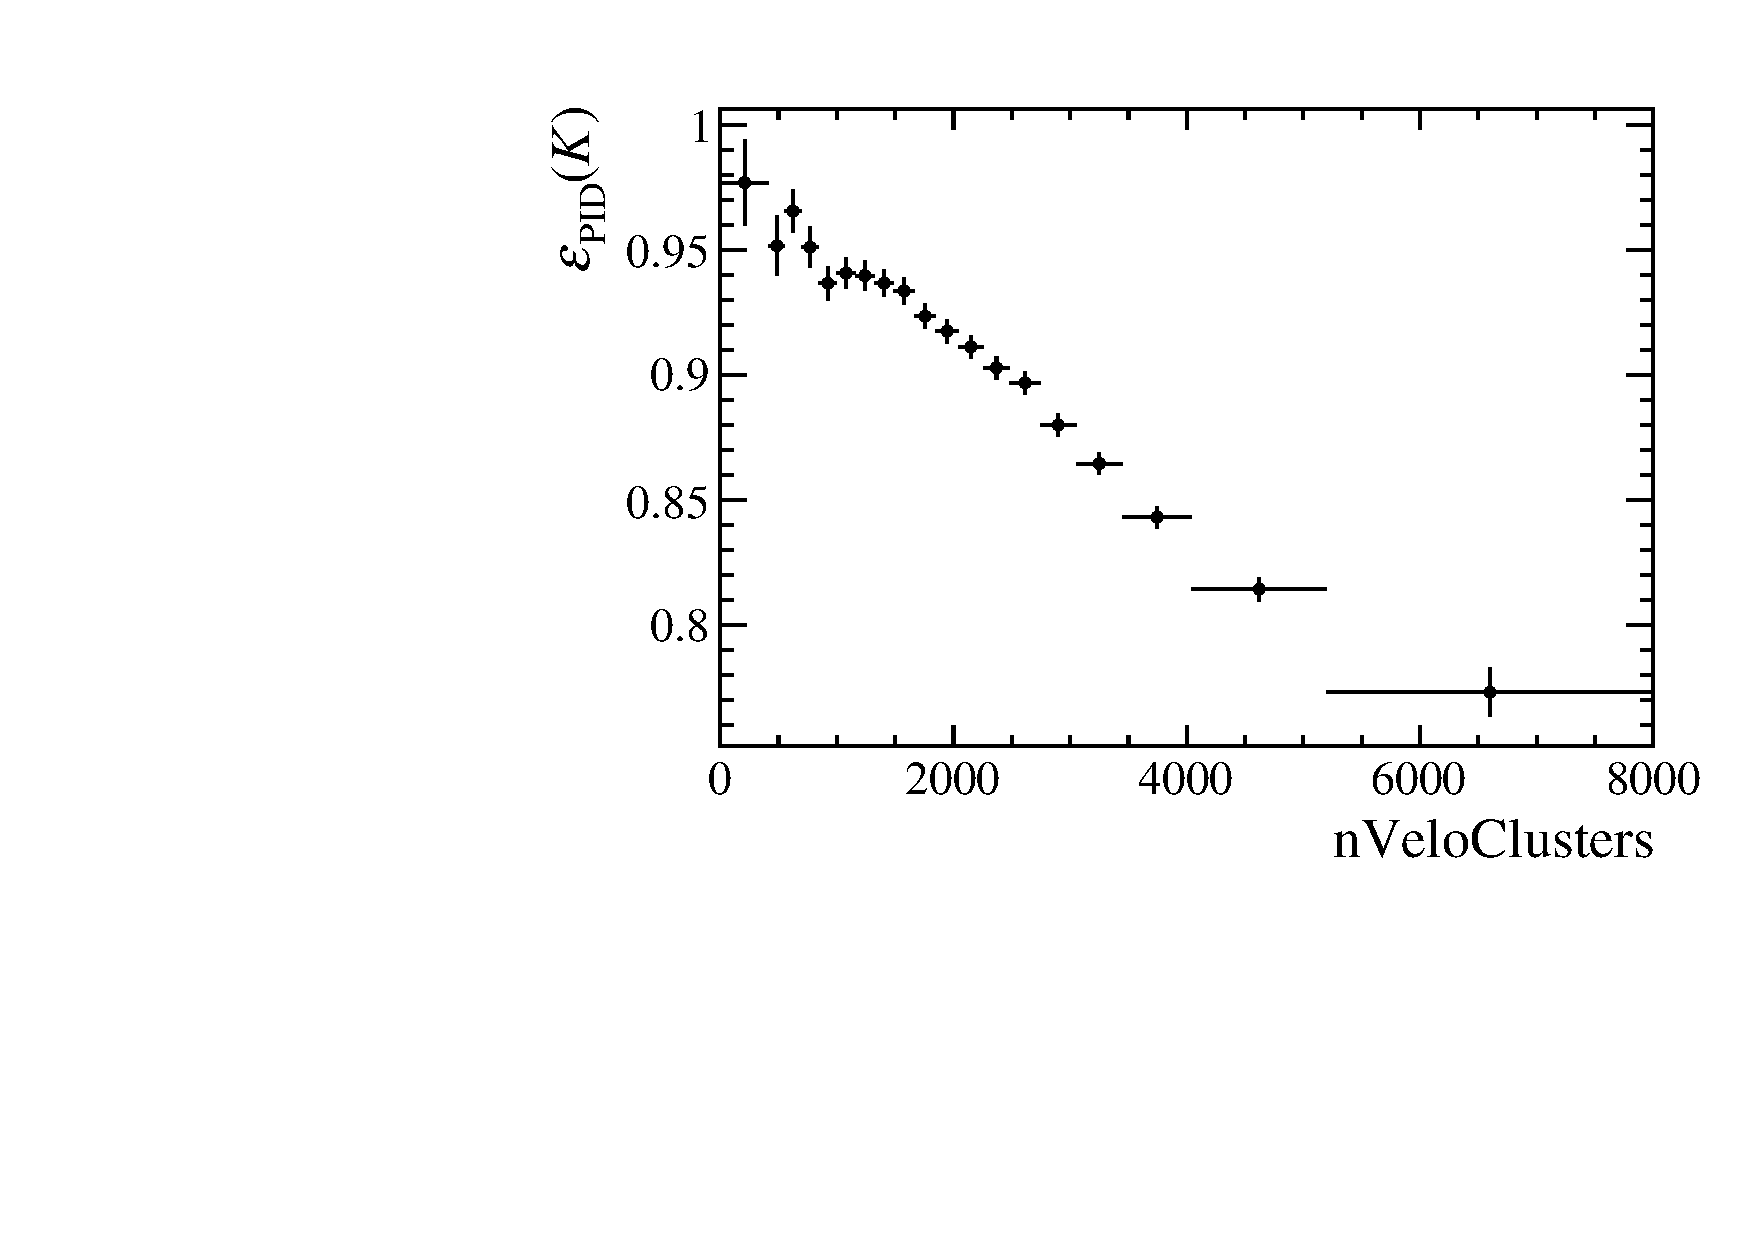
\includegraphics[width=0.45\linewidth]{PID/K_PID_nv_Ap}\put(-40,140){(d)}
    %\vspace*{-0.5cm}
    \caption{\small
    $\varepsilon_\mathrm{PID}(\kaon)$ as functions of (top) $(p,\eta)$ and (bottom) $\nVeloClusters$
    in (left) forward and (right) backward rapidites.
    }
    \label{fig:PID2DK}
\end{figure}
\begin{figure}[htbp]
    \centering
    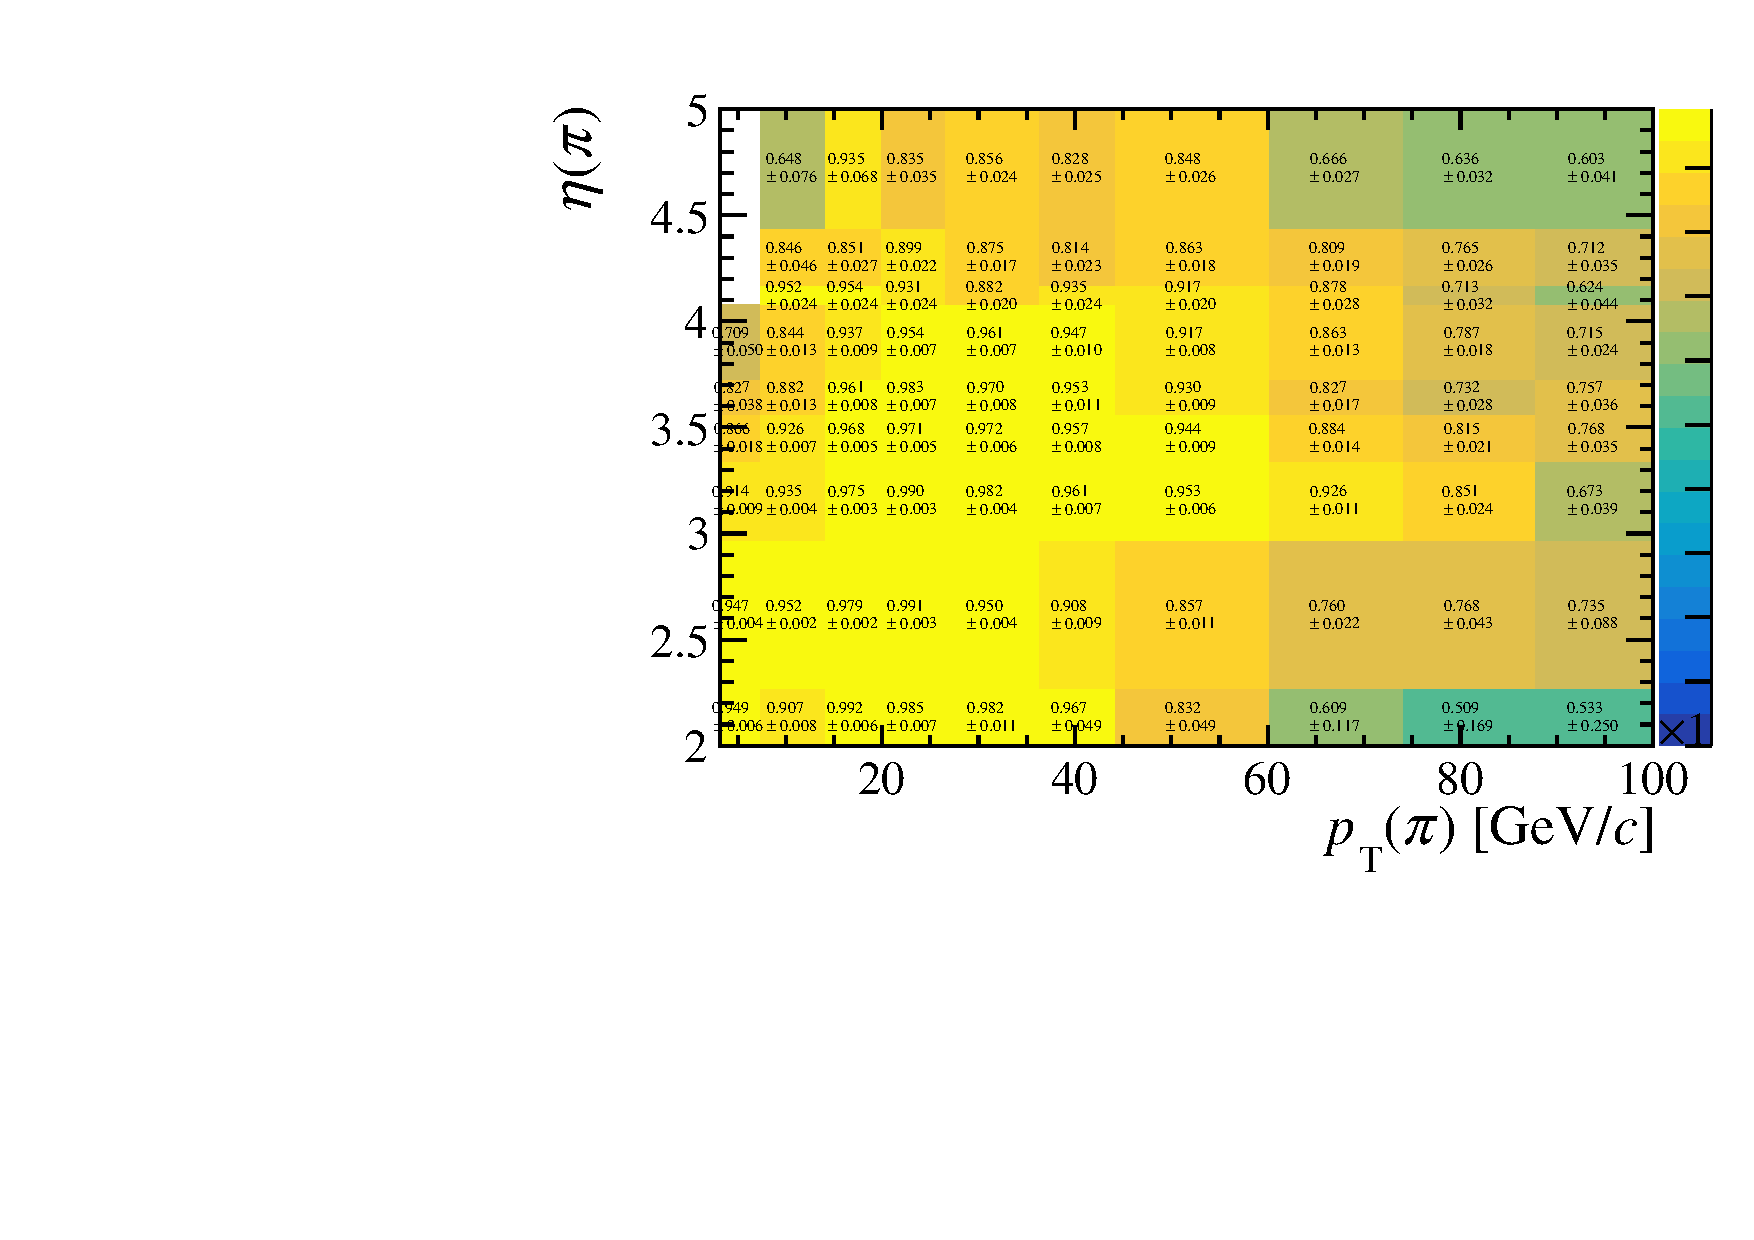
\includegraphics[width=0.45\linewidth]{PID/Pi_PID_p_eta_pA}\put(-40,140){(a)}
    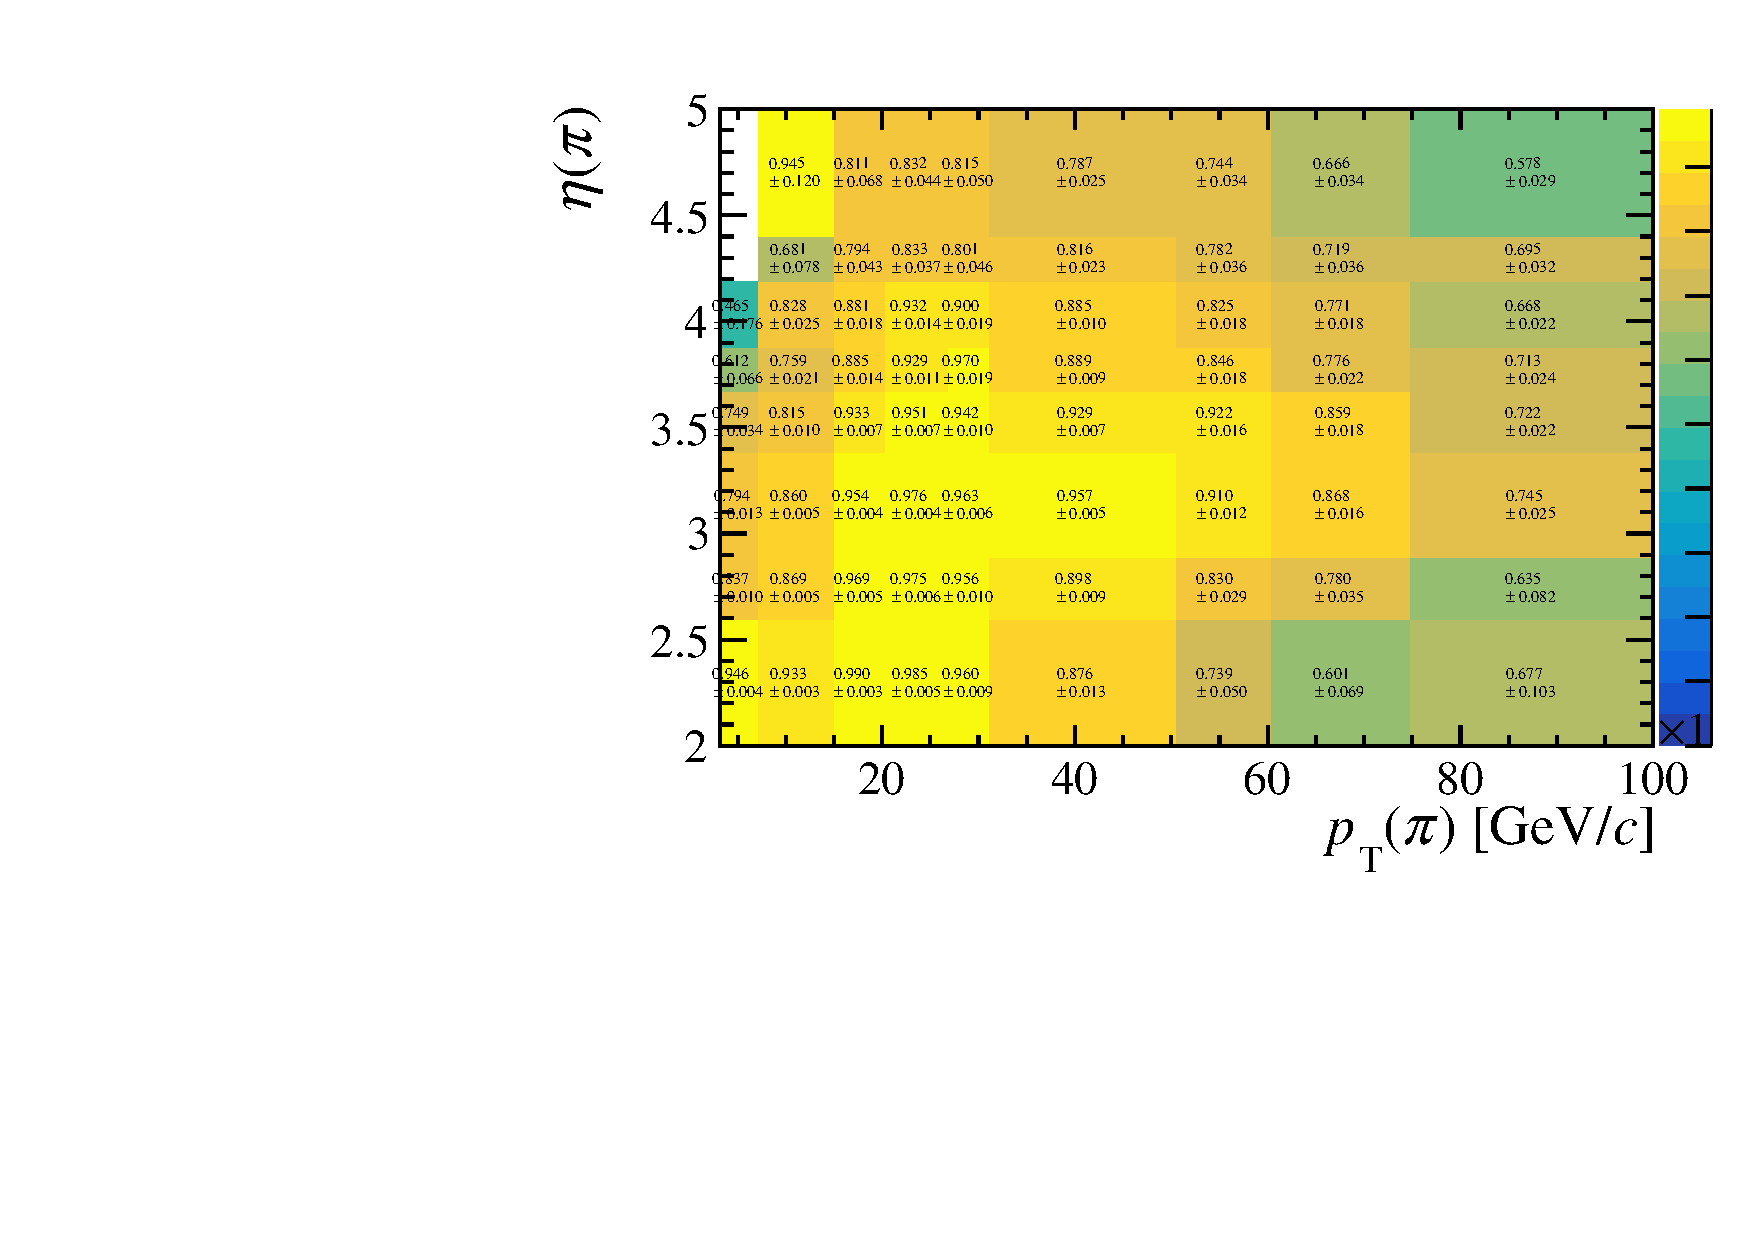
\includegraphics[width=0.45\linewidth]{PID/Pi_PID_p_eta_Ap}\put(-40,140){(b)}

    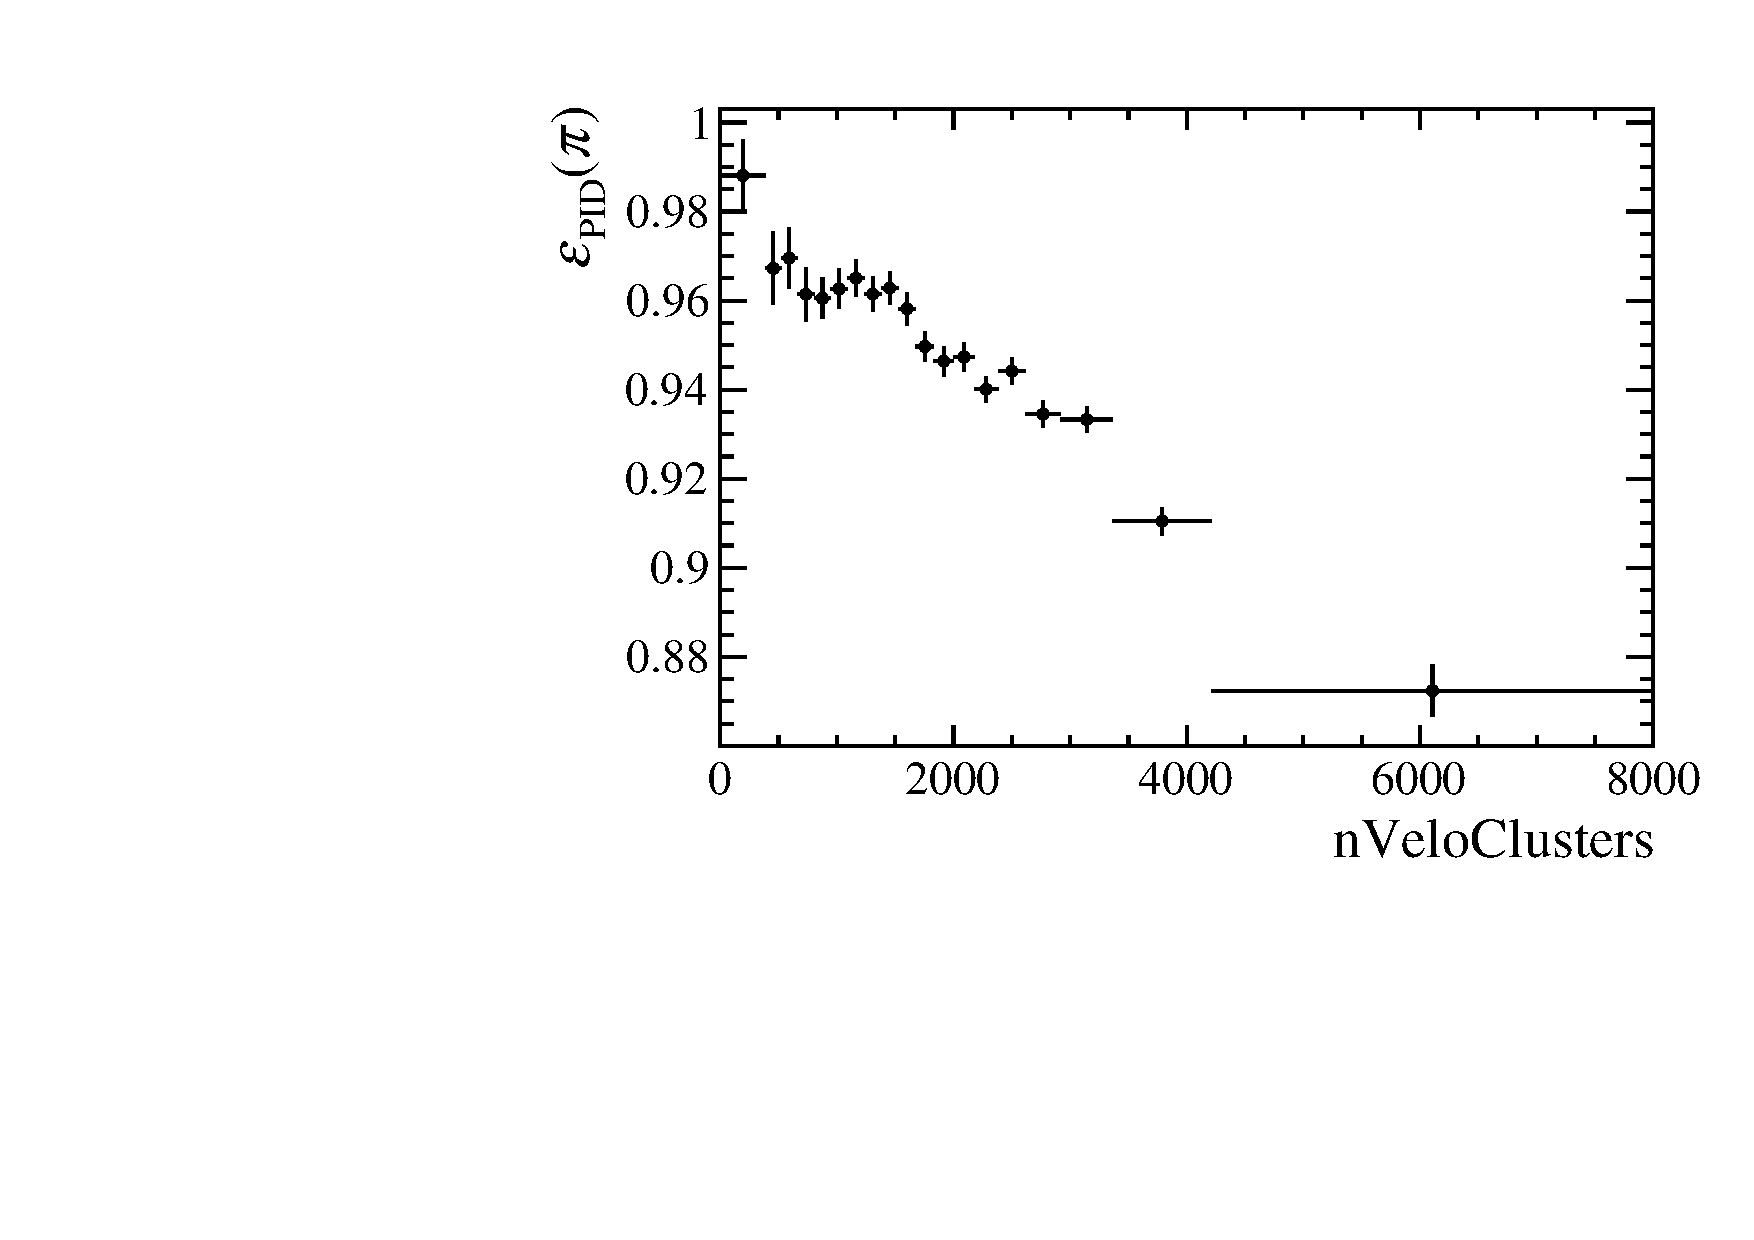
\includegraphics[width=0.45\linewidth]{PID/Pi_PID_nv_pA}\put(-40,140){(c)}
    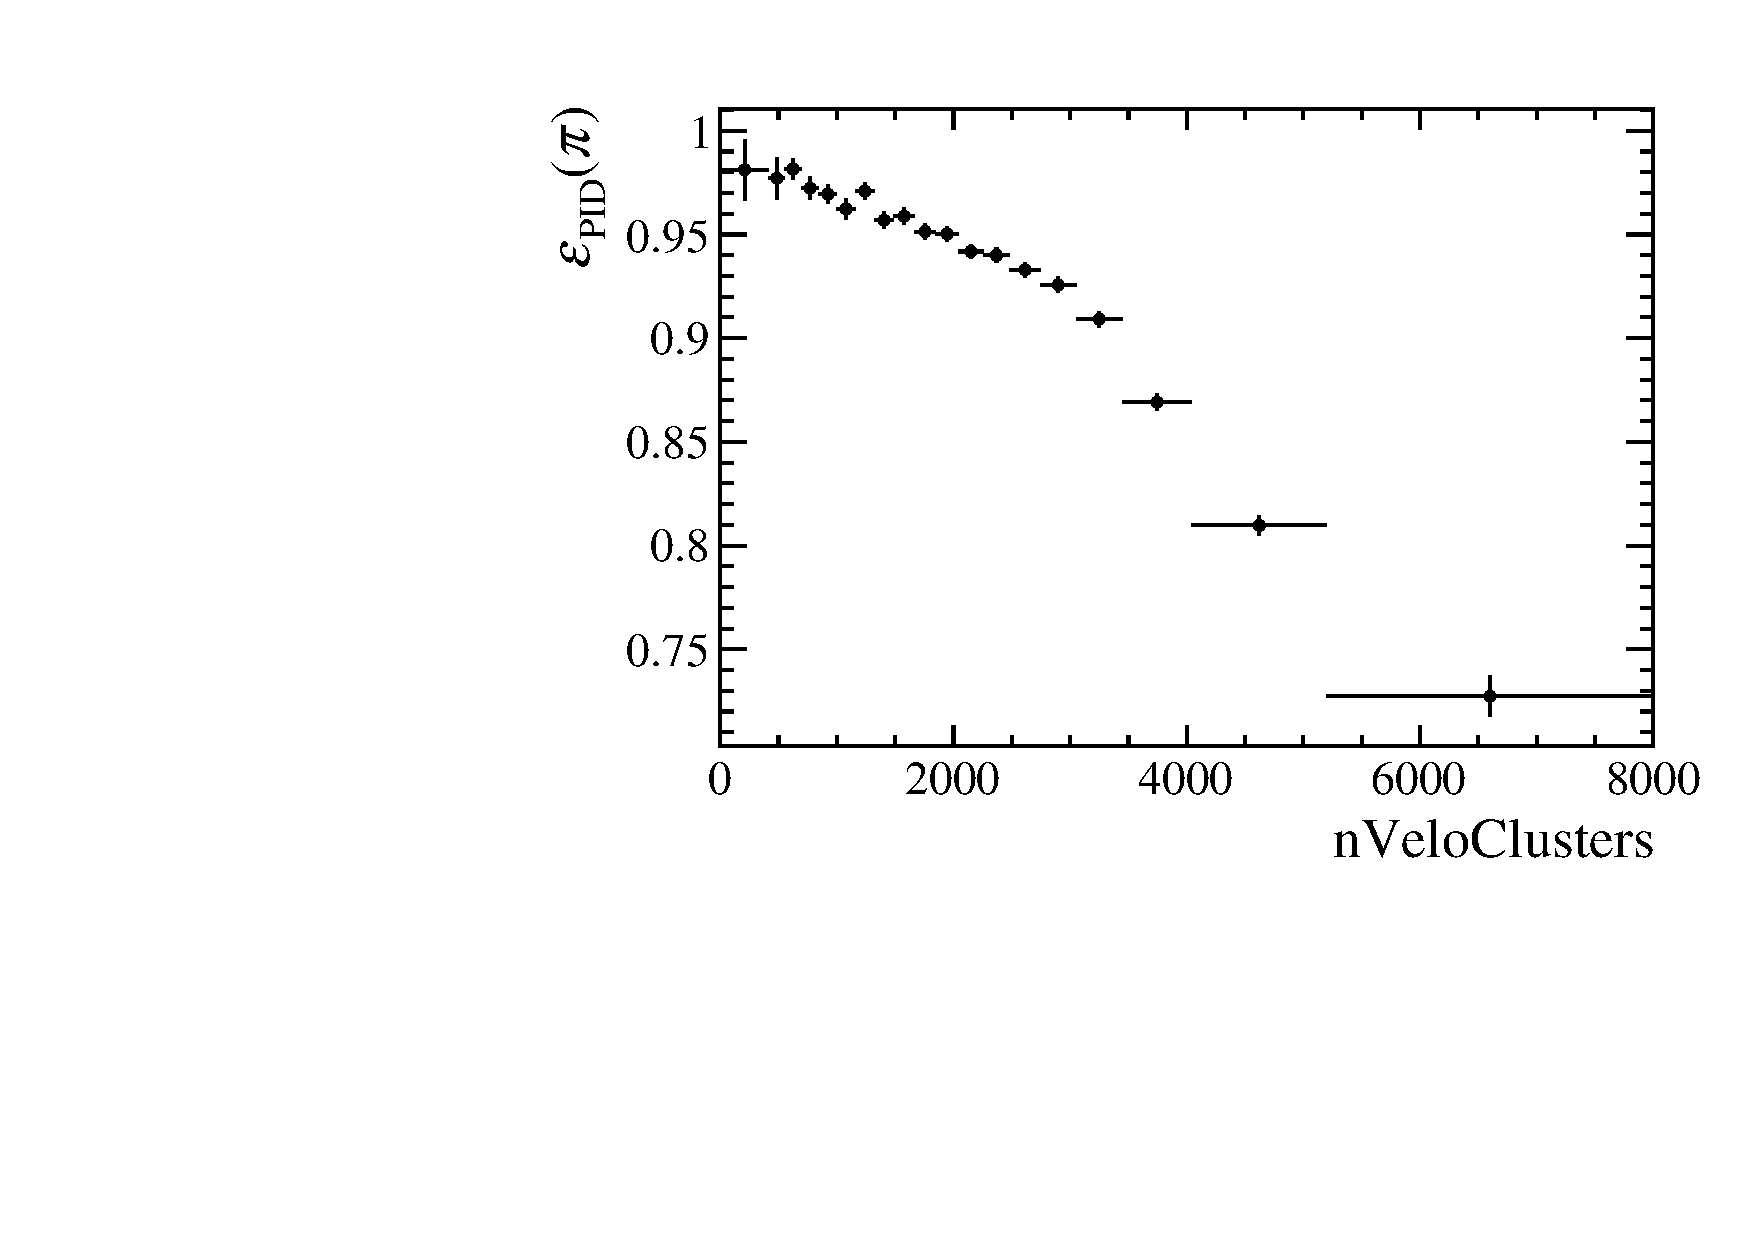
\includegraphics[width=0.45\linewidth]{PID/Pi_PID_nv_Ap}\put(-40,140){(d)}
    %\vspace*{-0.5cm}
    \caption{\small
    $\varepsilon_\mathrm{PID}(\pion)$ as functions of (top) $(p,\eta)$ and (bottom) $\nVeloClusters$
    in (left) forward and (right) backward rapidites.
    }
    \label{fig:PID2Dpi}
\end{figure}
For \proton, the correlation between kinematic and multiplicity variables does exist.
Fortunately, the corresponding calibration samples have more than $8\mathrm{M}$ candidates,
so three-dimensional tables can be directly obtained from these samples.
Projections of the table to the kinematic and multiplicity axes are also shown in Fig.~\ref{fig:PID2Dp}
to see an approximate value in each regions.
As the $\varepsilon_\mathrm{PID}(\proton)$ shows strong dependence on $p(\proton)$,
the bin widths there are set much smaller.
\begin{figure}[htbp]
    \centering
    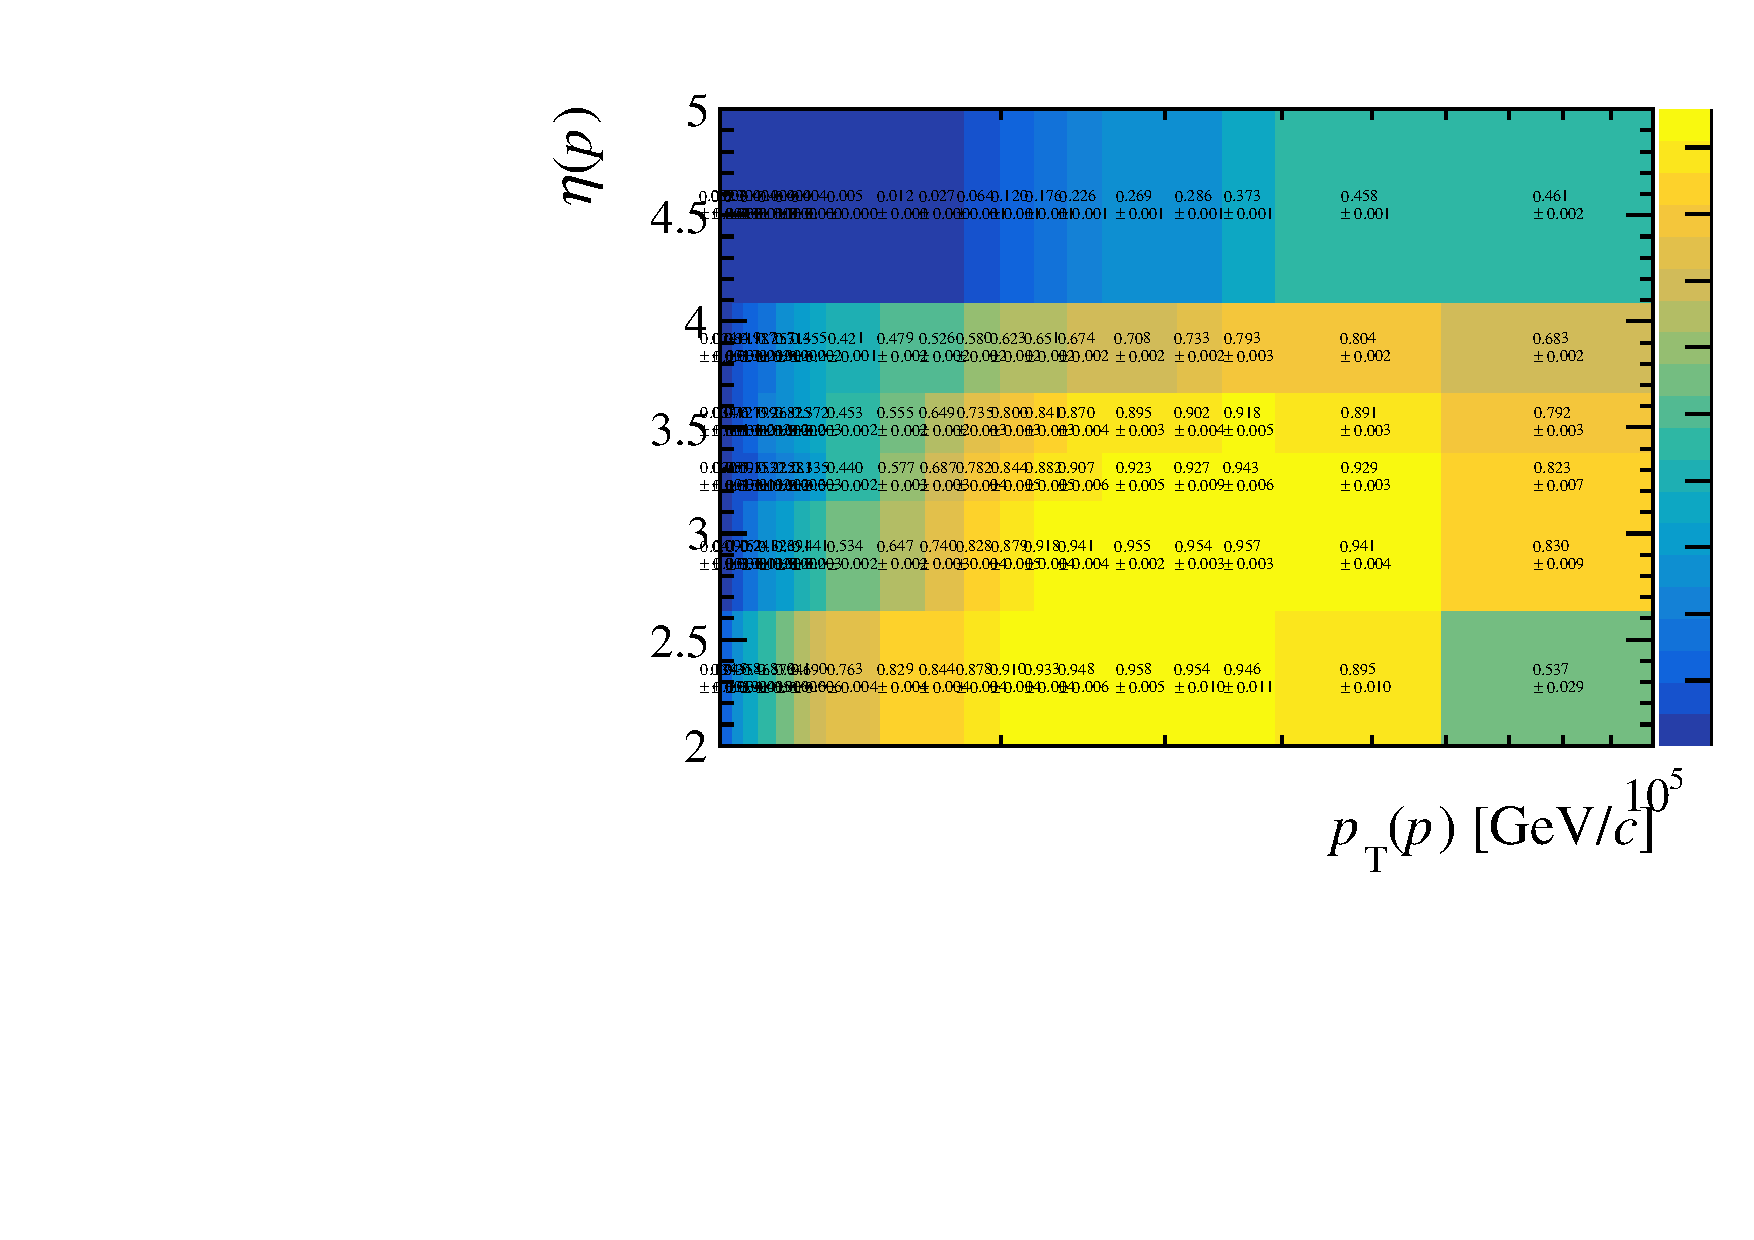
\includegraphics[width=0.45\linewidth]{PID/P_PID_p_eta_pA}\put(-40,140){(a)}
    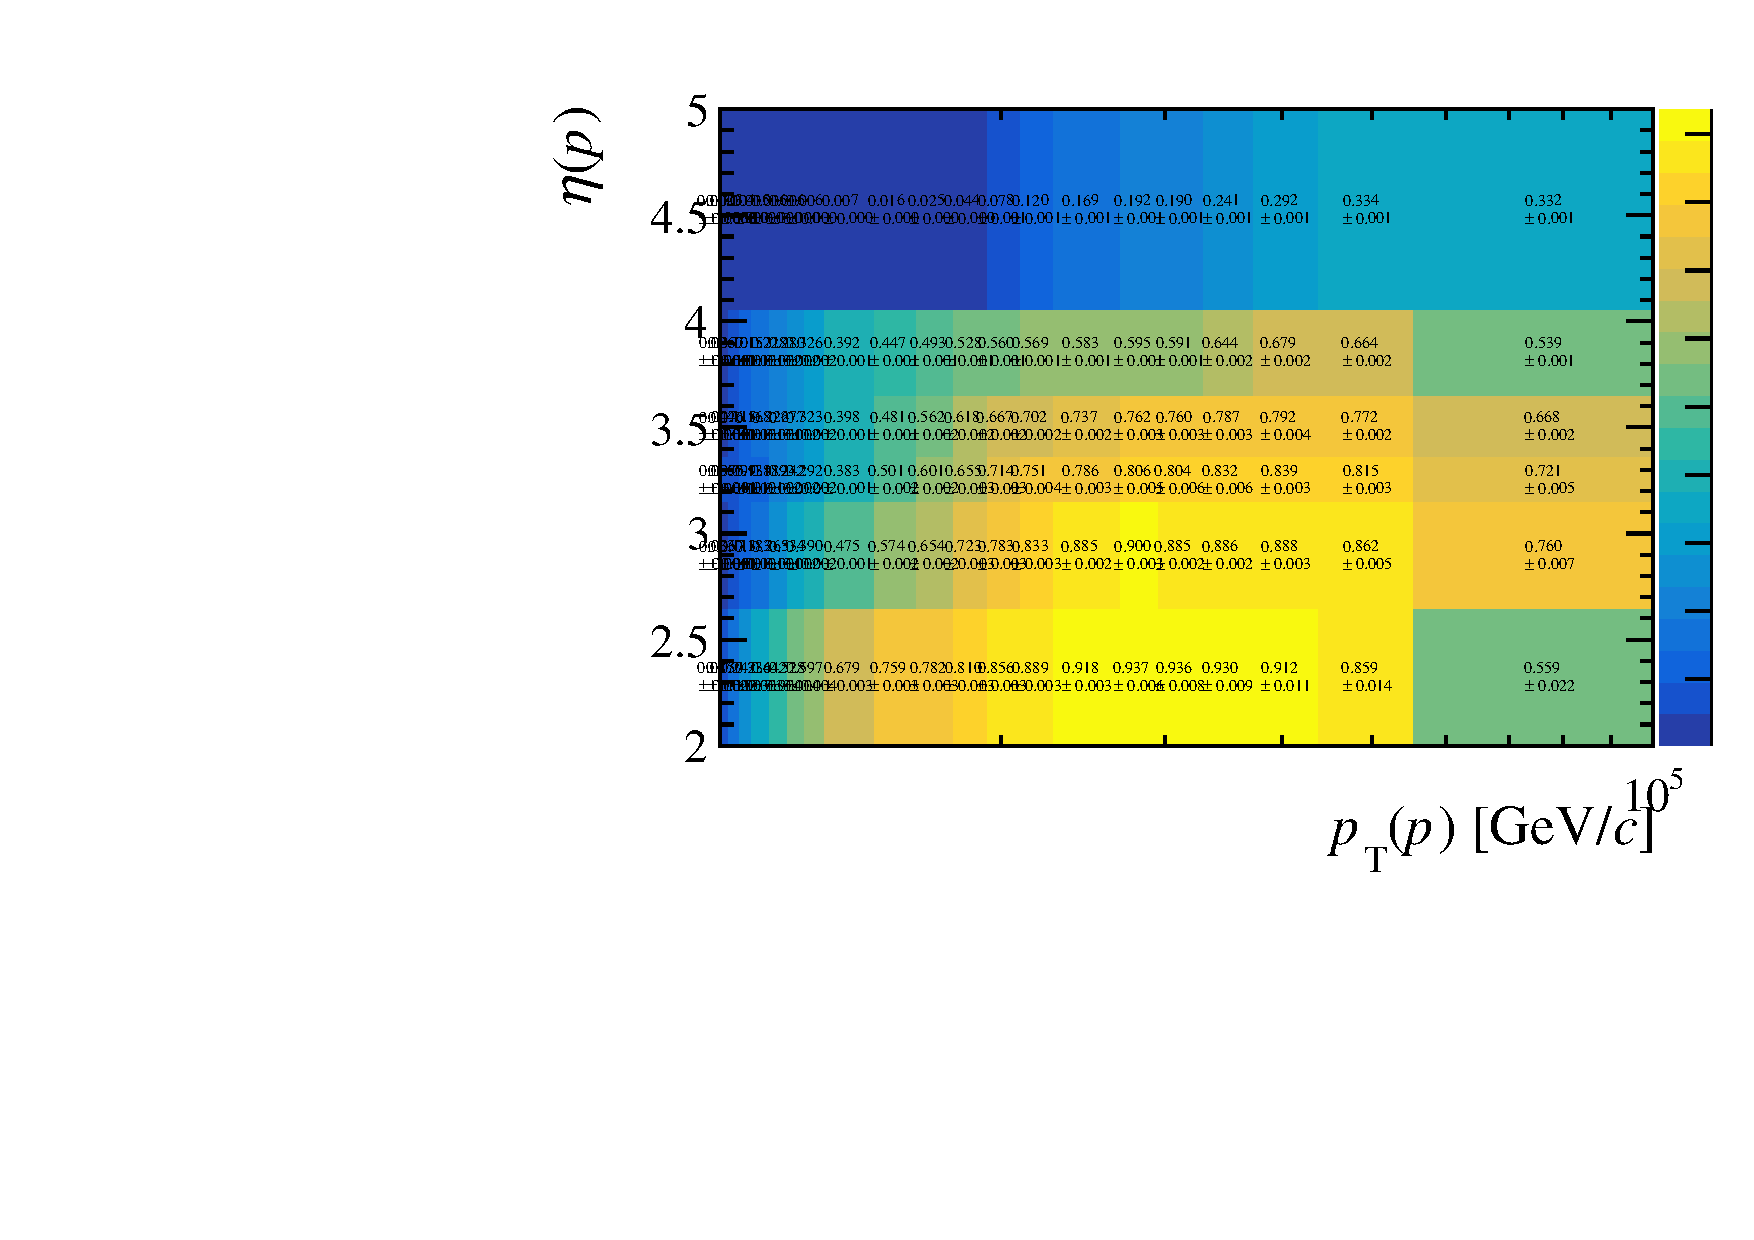
\includegraphics[width=0.45\linewidth]{PID/P_PID_p_eta_Ap}\put(-40,140){(b)}

    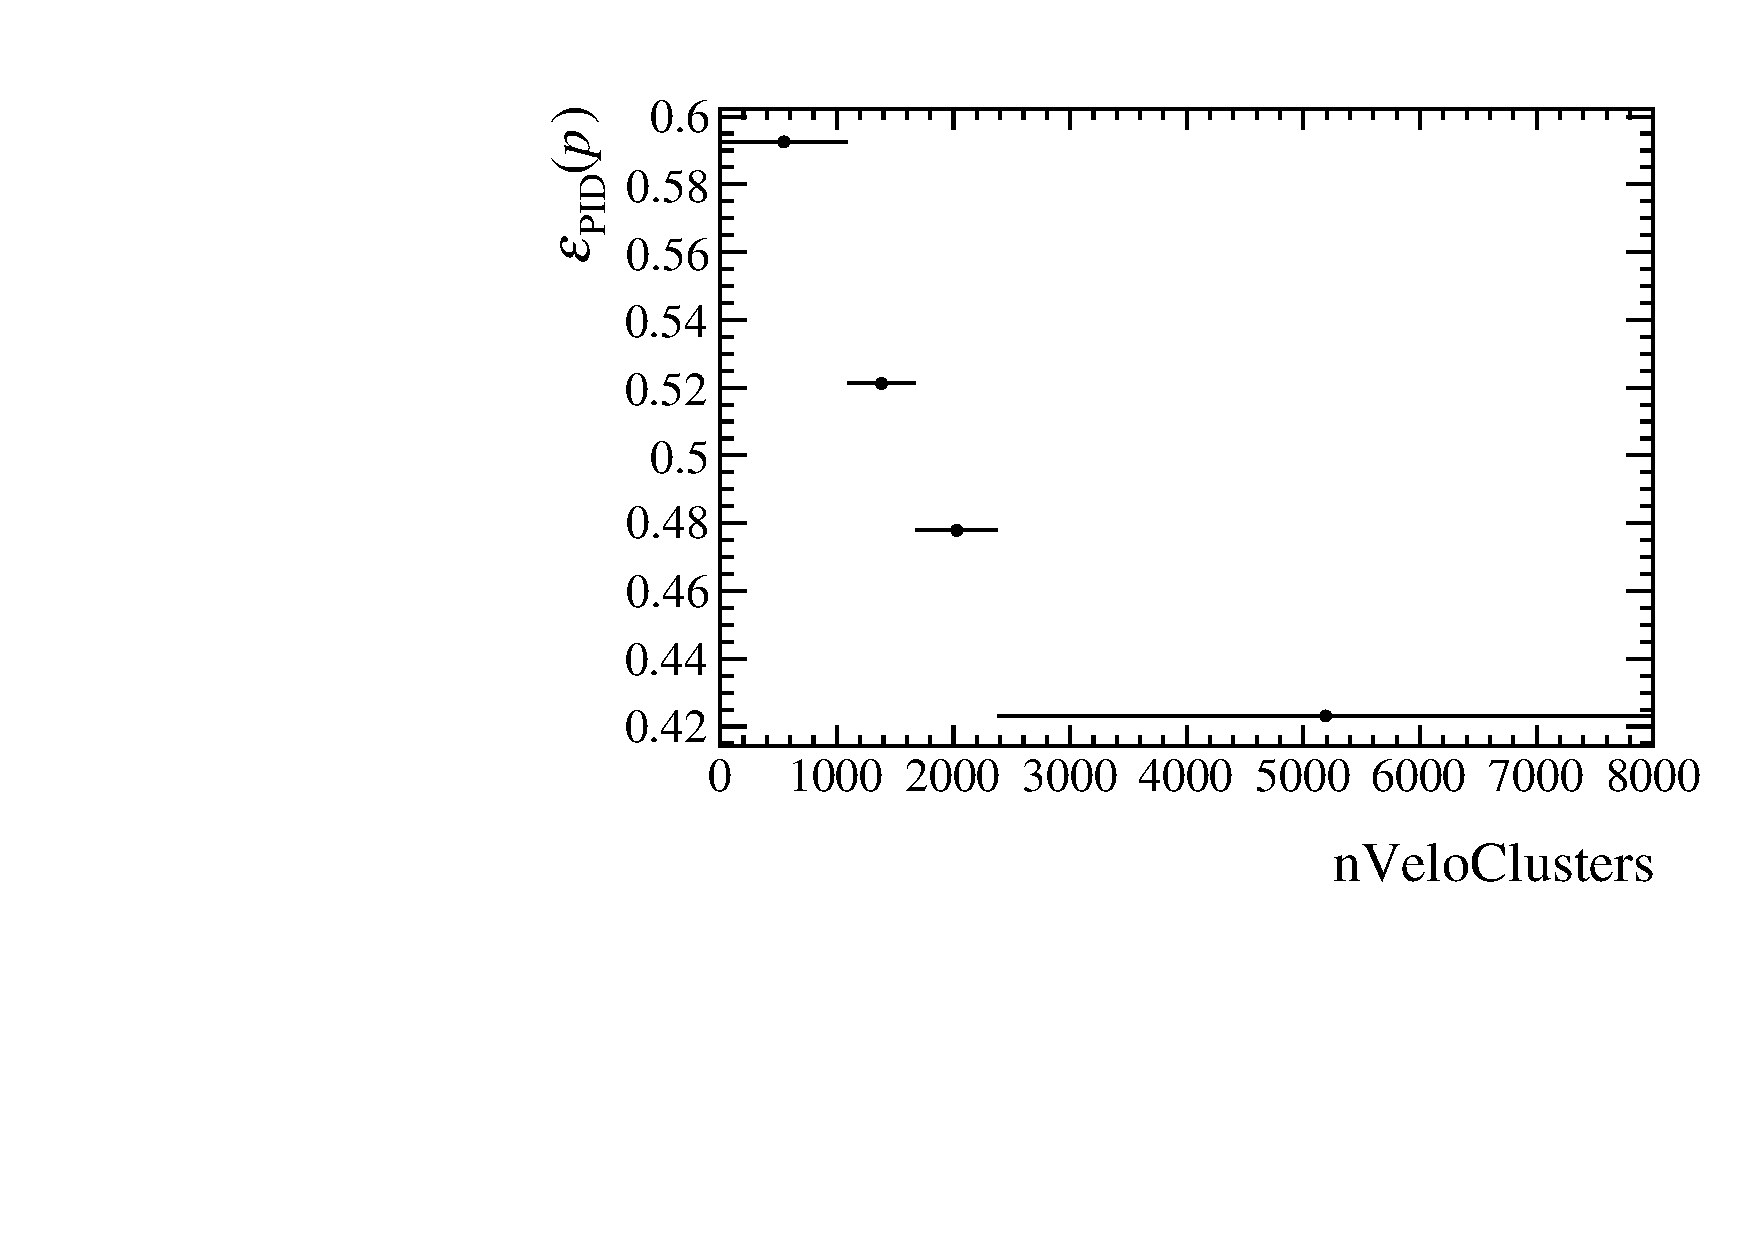
\includegraphics[width=0.45\linewidth]{PID/P_PID_nv_pA}\put(-40,140){(c)}
    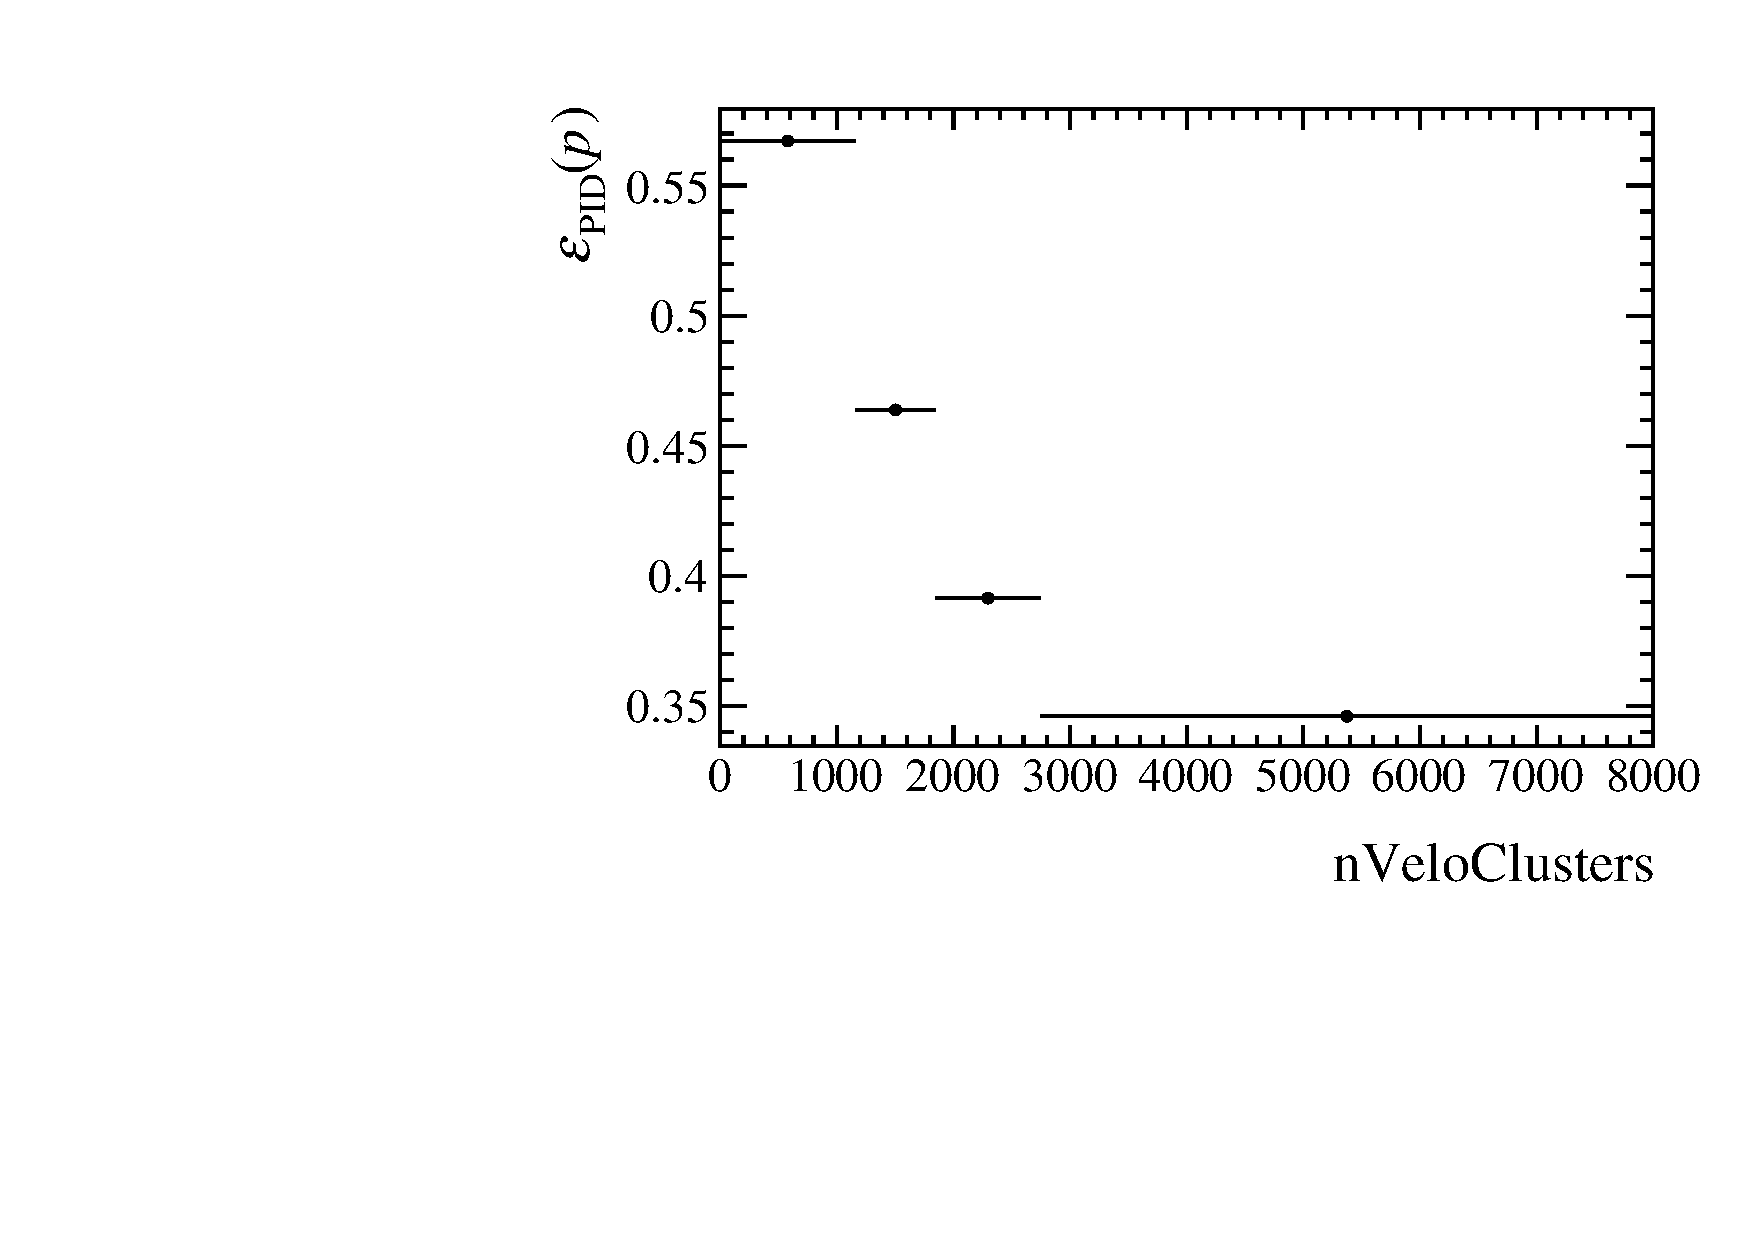
\includegraphics[width=0.45\linewidth]{PID/P_PID_nv_Ap}\put(-40,140){(d)}
    %\vspace*{-0.5cm}
    \caption{\small
    $\varepsilon_\mathrm{PID}(\proton)$ as functions of (top) $(p,\eta)$ and (bottom) $\nVeloClusters$
    in (left) forward and (right) backward rapidites. }
    \label{fig:PID2Dpi}
\end{figure}
With the calibration tables, $\varepsilon_\mathrm{PID}(\Lc)$ can be derived via Equation~\ref{eqn:eff_pid}.
Fig.~\ref{fig:eff_pid} show the results while the numerical values are listed in~\ref{tab:eff_PID2} in Appendix \ref{app:efficiency}.
\begin{figure}[htbp]
    \begin{center}
        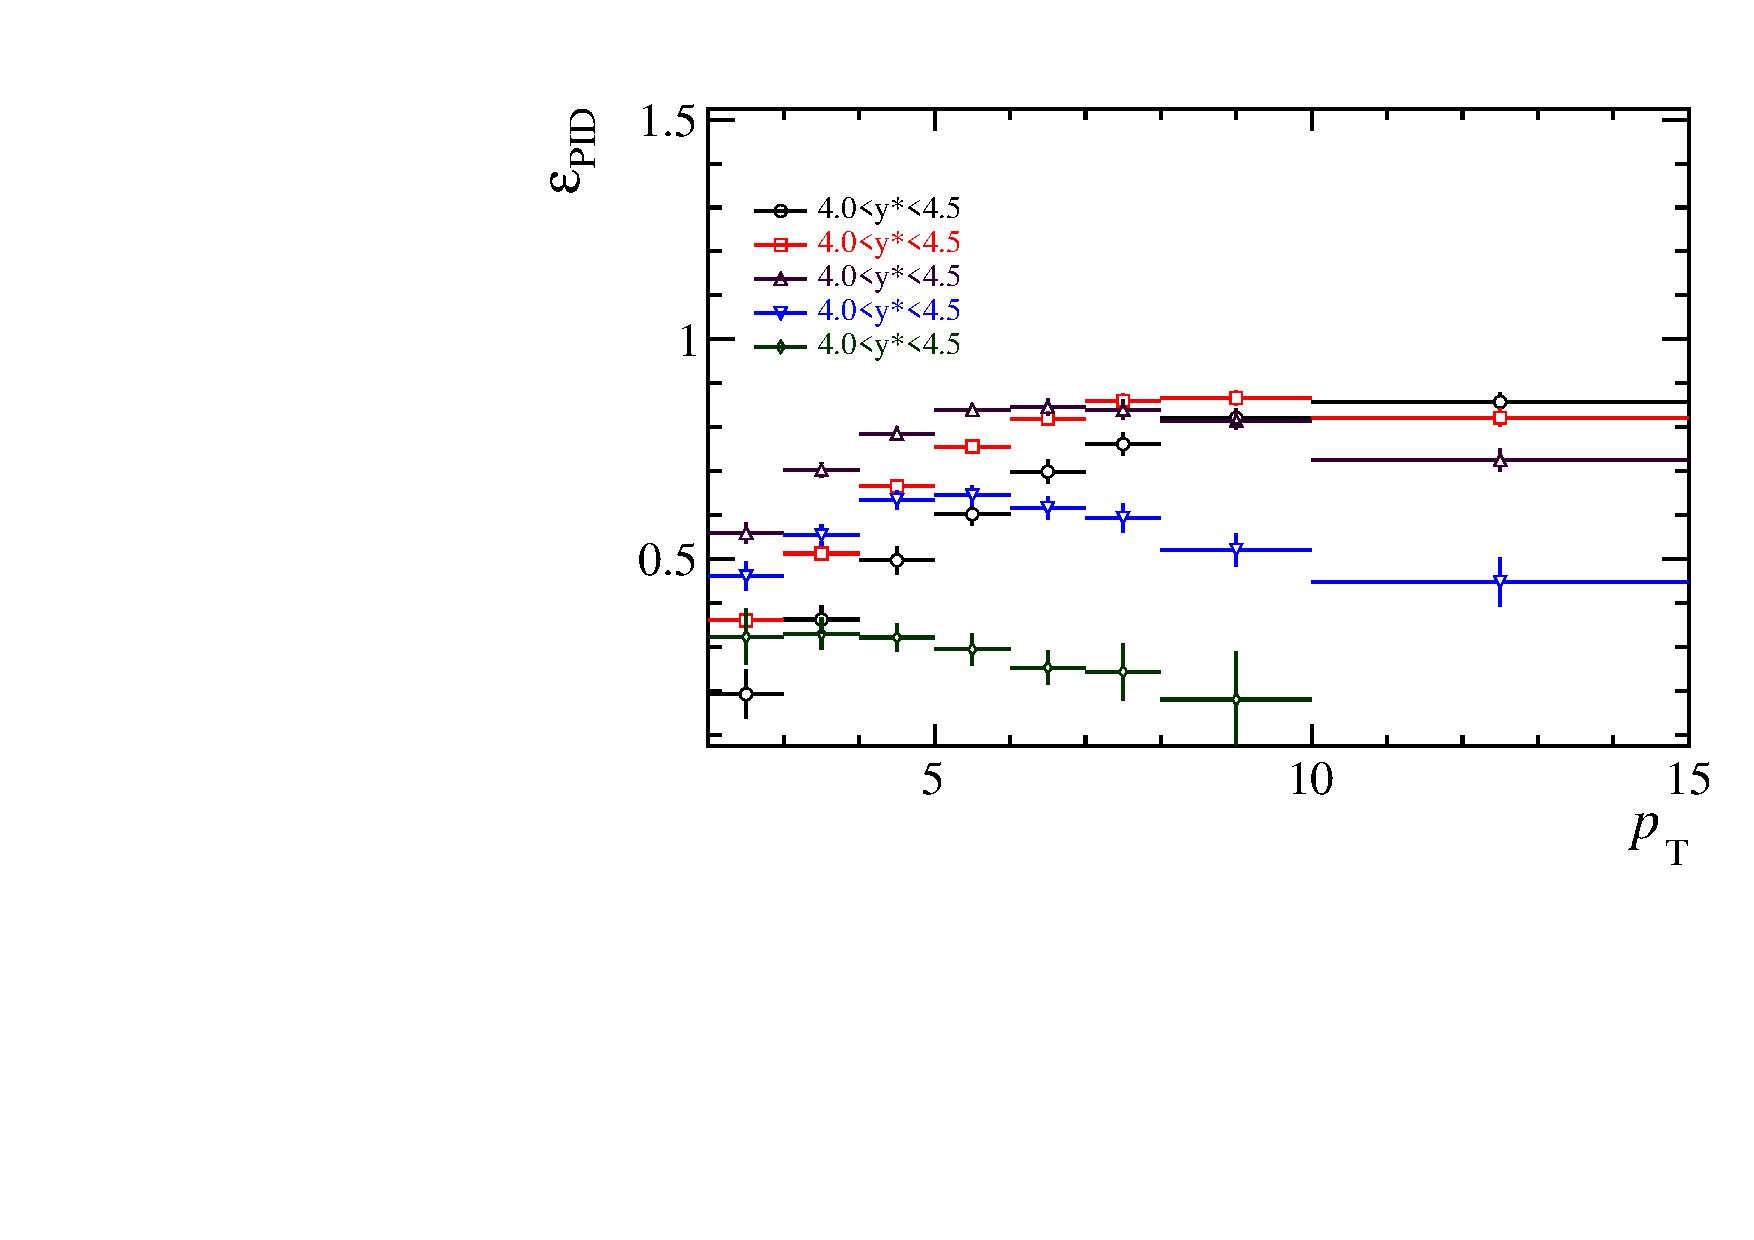
\includegraphics[width=0.45\linewidth]{plots/Lc_PID1}\put(-40,140){(a)}
        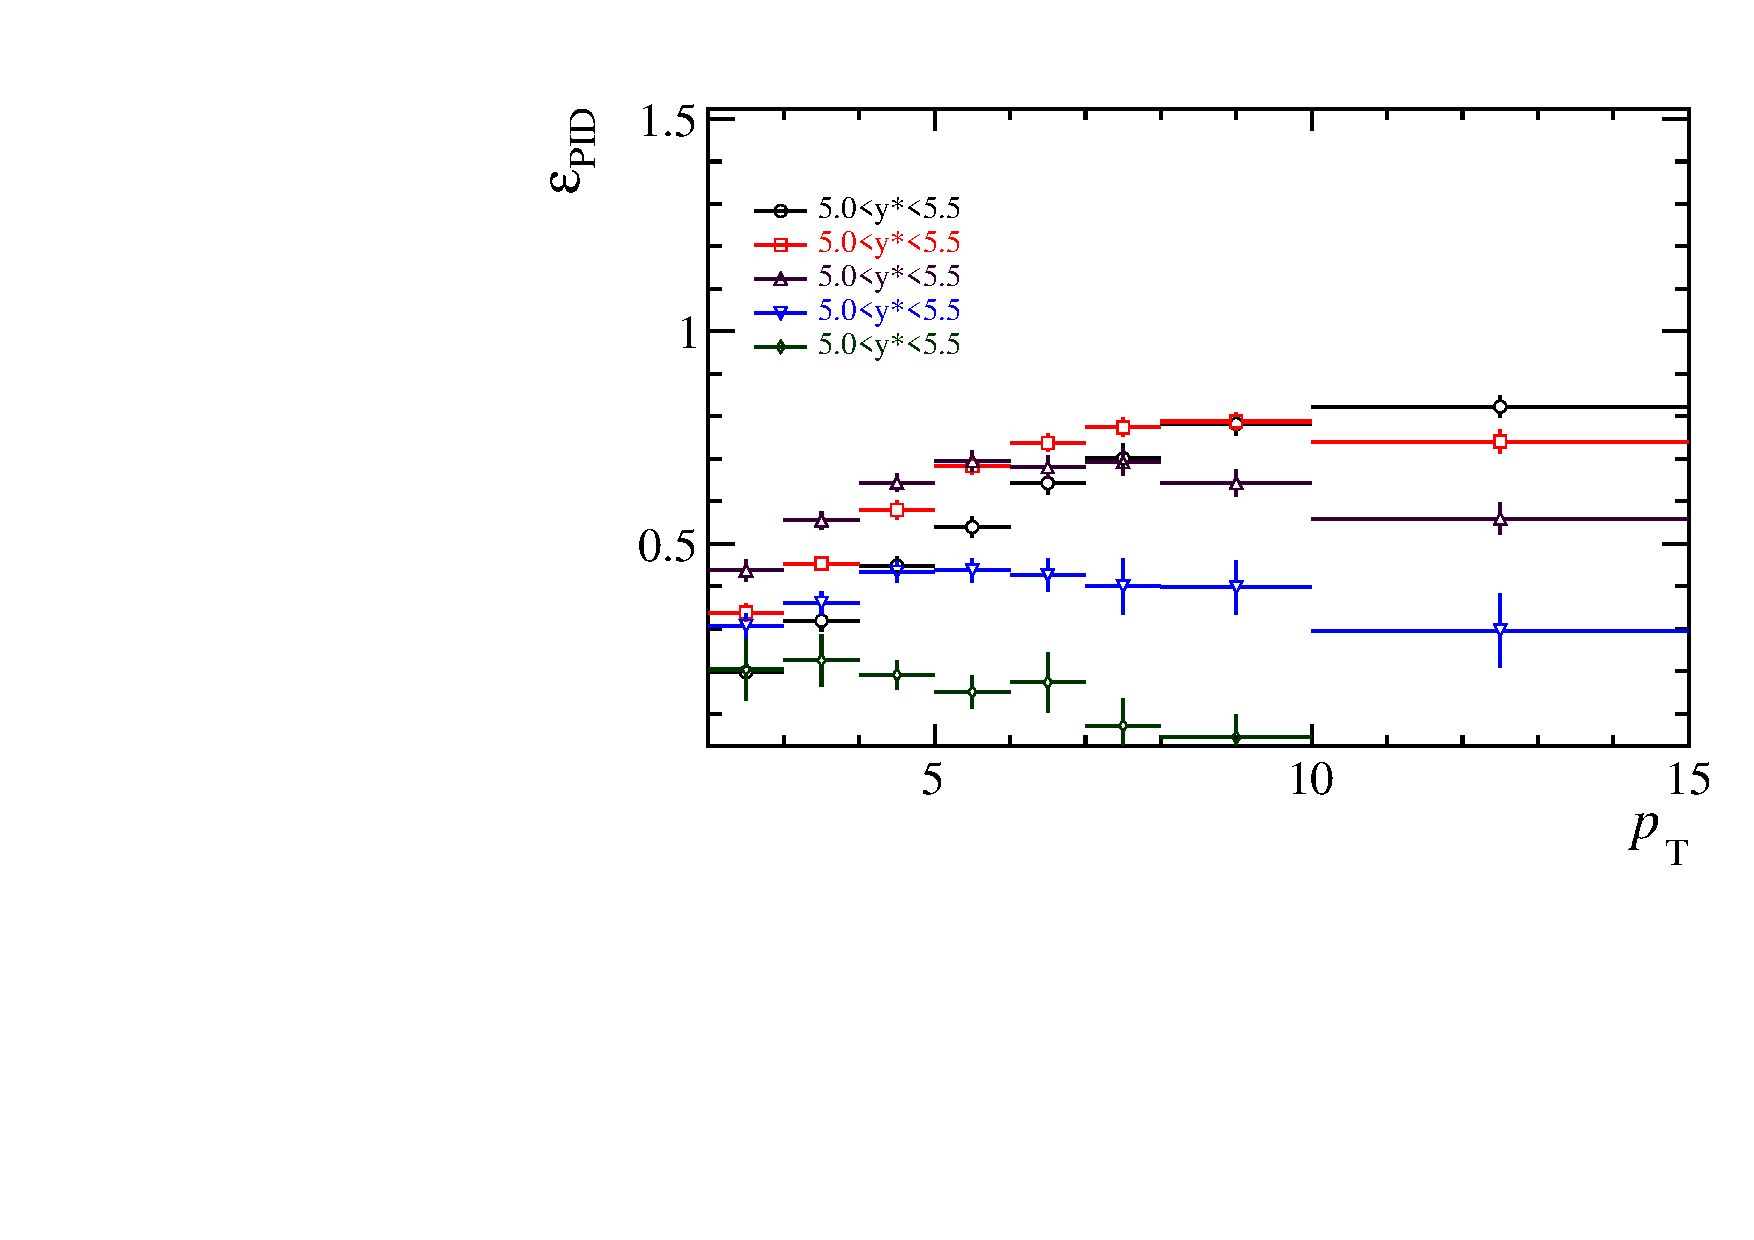
\includegraphics[width=0.45\linewidth]{plots/Lc_PID2}\put(-40,140){(b)}
        \vspace*{-0.5cm}
    \end{center}
    \caption{\small
    The PID efficiency $\varepsilon_\mathrm{PID}$ as a function of \pt and $y^*$ of prompt \Lc baryon
    for (left) forward and (right) backward rapidities. Statistical uncertainties only.}
    \label{fig:eff_pid}
\end{figure}

\subsection{Trigger efficiency}
As mentioned above, the triggers in this sample include L0, HLT1 and HLT2.
The {\tt L0SPD} is a minimum-biased trigger, so the efficiency is 1.
The other two selections are considered in \effsel.

\subsection{Total efficiency}
The total efficiencies are obtained directly from the multiplication of
the efficiencies above as Equation \ref{eqn:eff_total}.
The results are plotted on Fig.~\ref{fig:eff_total}
and listed in Table~\ref{tab:eff_tot1} and~\ref{tab:eff_tot2},
\begin{figure}[tb]
    \begin{center}
        \includegraphics[width=0.45\linewidth]{plots/Lc_Tot1}\put(-40,140){(a)}
        \includegraphics[width=0.45\linewidth]{plots/Lc_Tot2}\put(-40,140){(b)}
        \vspace*{-0.5cm}
    \end{center}
    \caption{\small
    The total efficiency \efftot~ as a function of \pt and $y^*$ of prompt \Lc baryon
    for (left) forward and (right) backward rapidities.}
    %Error bars are obtained from adding the statistical uncertainties all above in quadrature.}
    \label{fig:eff_total}
\end{figure}
\clearpage
